\documentclass{tudphygp_eng}
\usepackage{tudphymd,mhchem}
% \documentclass[12pt,a4paper]{scrartcl}
%\documentclass[12pt, a4paper]{article}
\usepackage[english]{babel}
% \usepackage[ansinew]{inputenc}
\usepackage{setspace}
\usepackage[T1]{fontenc}
\usepackage{lmodern}
\usepackage{cancel}
\usepackage{graphicx}
\usepackage{picins}
\usepackage{subfigure}
\usepackage{capt-of}
\usepackage{geometry}
\geometry{a4paper, left = 25mm, right = 20mm, top = 20mm, bottom = 20mm}
\usepackage[pict2e, verification]{struktex}
\usepackage{wasysym}
\usepackage{units}
\usepackage[pdftex]{hyperref} 

\addtokomafont{disposition}{\rmfamily}
\renewcommand{\baselinestretch}{1.2}\normalsize
\newcommand{\eigen}[1]{\textnormal{\textsc{#1}}}
\DeclareMathSizes{12}{12}{10}{10}

\versuch{Radiometrie 1 - Geiger M�ller counter tube}{RM1}
\author{PD Dr. J. Henniger, Dr. R. Schwierz, F. Hartung}
\bearbeitet{engl. R. Mertzig}{}
\date{Stand: 09.07.2013}



\begin{document}
% \title{Manual of the experiment \\ \textbf{\grqq RM1 -- }\eigen{Geiger-M�ller}-counter tube\grqq~}
% \author{Institut f�r Kern- und Teilchenphysik\\~ \\ Created by: \\ PD Dr. J�rgen Henniger \\ Dr. Rainer Schwierz \\ ~ \\ edited by: \\ Franz Hartung}
% \date{Effective: 09.07.2013}
\maketitle


\section{Task}
The concentration of a \textsf{K}$_2$\textsf{CO}$_3$-solution has to be determined through its activity after determining the characteristics of the \eigen{Geiger-M�ller}-counter tube (GMC) and the relative responsivity of the corresponding experiment setup. 

\section{Basics}

\subsection{Radioactivity and the law of decay}

Atoms consist of a positively charged nucleus and a negatively charged shell. \\
The nucleus is composed of \textit{nucleons}: the \textit{protons} (symbol~$p$) and \textit{neutrons} (symbol~$n$). \\
The \textit{electrons} (symbol~$e^-$) constitute the shell.\\[0,3 cm]
The different atoms were allocated in categories called \textit{nuclides}. They were distinguished by number and and kind of the nucleons in the nucleus. A certain nuclide has a defined \textit{nucleon number} $A$ and a certain \textit{neutron number} $N$. The difference $Z = A - N$ equals the number of protons in the nucleus as well as the number of the electrons in the shell, a result of the electrical neutrality of the atom from outside. $Z$ is defined as the \textit{atomic number}. \\

All these numbers are summarized in the notation $^A_Z$\textsf{X}$^{~}_N$ or shortly $^A_Z$\textsf{X} resp. $^A$\textsf{X} with \textsf{X} as the chemical symbol. For instance $^4_2$\textsf{He}$^{~}_2$ is helium with a nucleus consisting of two protons and two neutrons. \\[0,3cm]

Not all nuclei are in a stable state. The phenomena \textit{radioactivity} is the spontaneous transmutation of non-stable nuclei with energy emission. 
The transmutation-related transition into a stable nucleus can be made directly or in many sequential steps. The energy will be emitted through ionizing radiation either by particles and/or photons. That can be generated directly in the nucleus or indirectly in the atomic shell. \\
There are different types of transmutations, which are also summarized in table \ref{tab_umwandlungsarten} :

\begin{description}
	\item[$\alpha$-decay:] Heavy elements with a low binding energy of the nucleons in the nucleus can be transmuted by emitting of a $^4_2$\textsf{He}-nucleus ($\alpha$-radiation). Spontaneous fission is also a radioactive transmutation. 
	\item[$\beta$-decay:] Nuclei with an unfavorable neutron-proton ratio are transmuted through $\beta$-transmutation or $e^-$-capture. Here the emission caused by a surplus of neutrons is defined as $\beta^-$-radiation, if an electron is emitted, and $\beta^+$-radiation, if a positron is emitted. The $e^-$-capture, where a shell electron is captured by the nucleus, is an alternative to the $\beta^+$-transmutation.  
	\item[$\gamma$-radiation:] Excited nuclei can be generated during all previously described transmutations. These nuclei can decay into a stable ground state through the emission of a photon ($\gamma$-radiation)
 
\end{description}

The change of the atomic number due to the transmutation of the nuclei makes it necessary to rearrange the shell structure of the electrons.
The result is the emission of characteristic \textit{x-rays} and/or \eigen{Auger}\textit{-electrons}. 
An emission of $K_\alpha$- and $K_\beta$ x-rays due to the created vacancy in the K-shell can be observed distinctly for electron capture.\\

\begin{center}
\begin{minipage}{1 \textwidth}
\captionof{table}{Types of decay (without spontaneous fission)} \label{tab_umwandlungsarten}~\\
\centering
\begin{tabular}{c c c}
Type of decay	&	Transmutation of the nucleus &	Transmutation within the nucleus \\ \hline ~\\
$\alpha$	&	$^A_Z$\textsf{X}$^{~}_N~\rightarrow~^{A-4}_{Z-2}$\textsf{Y}$^{~}_{N-2} ~+~ ^4_2$\textsf{He}$^{~}_2$	&	Clustering \\[0,4cm]
$\beta^-$	&	$^A_Z$\textsf{X}$^{~}_N~\rightarrow~^{A}_{Z+1}$\textsf{Y}$^{~}_{N-1} ~+~ e^- ~+~ \overline{\nu}$	&	$n$-surplus:~ $n \rightarrow~p + e^- + \overline{\nu}$ \\[0,4cm]
$\beta^+$	&	$^A_Z$\textsf{X}$^{~}_N~\rightarrow~^{A}_{Z-1}$\textsf{Y}$^{~}_{N+1} ~+~ e^+ ~+~ \nu$	&	$p$-surplus:~ $p \rightarrow~n + e^+ + \nu$ \\[0,4cm] 
$e^-$-capture	&	 $^A_Z$\textsf{X}$^{~}_N ~+~ e^- ~\rightarrow~^{A}_{Z-1}$\textsf{Y}$^{~}_{N+1} ~+~ \nu$	&	$p$-surplus:~ $p + e^- \rightarrow~n + \nu$ \\ \hline
\end{tabular}
\end{minipage}
\end{center} ~\\
~\\
These spontaneous processes have a stochastic origin, i.~e.: Every unstable nucleus has the same probability of transmutation, independent from its history, where the moment of its transmutation is undetermined. 
It is therefore not possible to predict the time when a certain nucleus will transmute. Only the probability of the transmutation event in a certain time interval is known. The number of the averagely occurring transmutations $\mathrm d N$ can be calculated for many equal, unstable nuclei $N$, which are present at the time $t$. For that the linear differential equation

\begin{eqnarray}
\mathrm d N &=& -\lambda \cdot N \cdot \mathrm d t \label{glg_zerfallsgegetz}
\end{eqnarray}
is applied. 
The nucleus specific \textit{decay constant} $\lambda$ is a degree of the transmutation probability of a radionuclide. Its inverse value $\tau = \nicefrac{1}{\lambda}$ is the average life time of the corresponding nucleus. By integrating (\ref{glg_zerfallsgegetz}) according to


\begin{eqnarray}
\int\limits^{N(t)}_{N_0}{\frac{\mathrm d N}{N}} &=& -\int\limits^t_0{\lambda \mathrm d t} ~~~~ \rightarrow ~~~~ \ln N(t) - \ln N_0 ~~=~~ -\lambda \cdot t \nonumber
\end{eqnarray}
the \textit{exponential decay law}
\begin{eqnarray}
N(t) &=& N_0 \cdot \mathrm e ^{-\lambda \cdot t} \label{glg_umwandlungsgesetz}
\end{eqnarray}
results. 

There is $N(t)$, the number of nuclei which are not transmuted at the time $t$, and $N_0 = N(t=0)$
is the number of nuclei at the time $t=0$. The solution of (\ref{glg_umwandlungsgesetz}) for the case $N(t = T_{1/2}) =\nicefrac{N_0}{2}$ is the \textit{half-life period}.

\begin{eqnarray}
T_{1/2} &=& \frac{\ln 2}{\lambda} ~~=~~ \tau \cdot \ln 2  ~~~~~. \label{glg_halbwertszeit}
\end{eqnarray}

The transmutation rate or \textit{activity} $A$ is the number of spontaneous decays per time unit. This rate is proportional to the number of unstable nuclei. Beginning at initial activity $A_0 = A(t=0)$ at the time $t=0$ one finds via

\begin{eqnarray}
A(t) &=& - \frac{\mathrm d N}{\mathrm d t} ~~=~~ \lambda \cdot N(t) \label{glg_aktivit�t_1} 
\end{eqnarray}
also an exponential correlation expressed as:
\begin{eqnarray}
A(t) &=& A_0 \cdot \mathrm e^{-\lambda \cdot t} \label{glg_aktivit�t_2}
\end{eqnarray}
This equation can be rewritten with (\ref{glg_halbwertszeit}) as
\begin{eqnarray}
A(t) &=& A_0 \cdot \left( \frac{1}{2} \right) ^{\frac{t}{T_{1/2}}} ~~~~~. \label{glg_aktivit�t_3} 
\end{eqnarray}
The unit of the activity is the \textit{Becquerel} (1 \textsf{Bq} = 1 \textsf{s}$^{-1}$).
The activity is the most important unit for characterizing a radioactive source other than the energy and kind of emitted radiation. The expression of the law of decay in (\ref{glg_aktivit�t_3}) with the factor $\nicefrac{1}{2}$ and $n = \nicefrac{t}{T_{1/2}}$ is especially easy to handle for experimentalists. 
Because the exponentiation $2^n$ sufficiently known from computer science (for instance $2^{20} \approx 10^6$), one can estimate calculations according to (\ref{glg_aktivit�t_3}) quite quickly.\\[0,3cm]
\begin{figure}[htbp]
\begin{center}
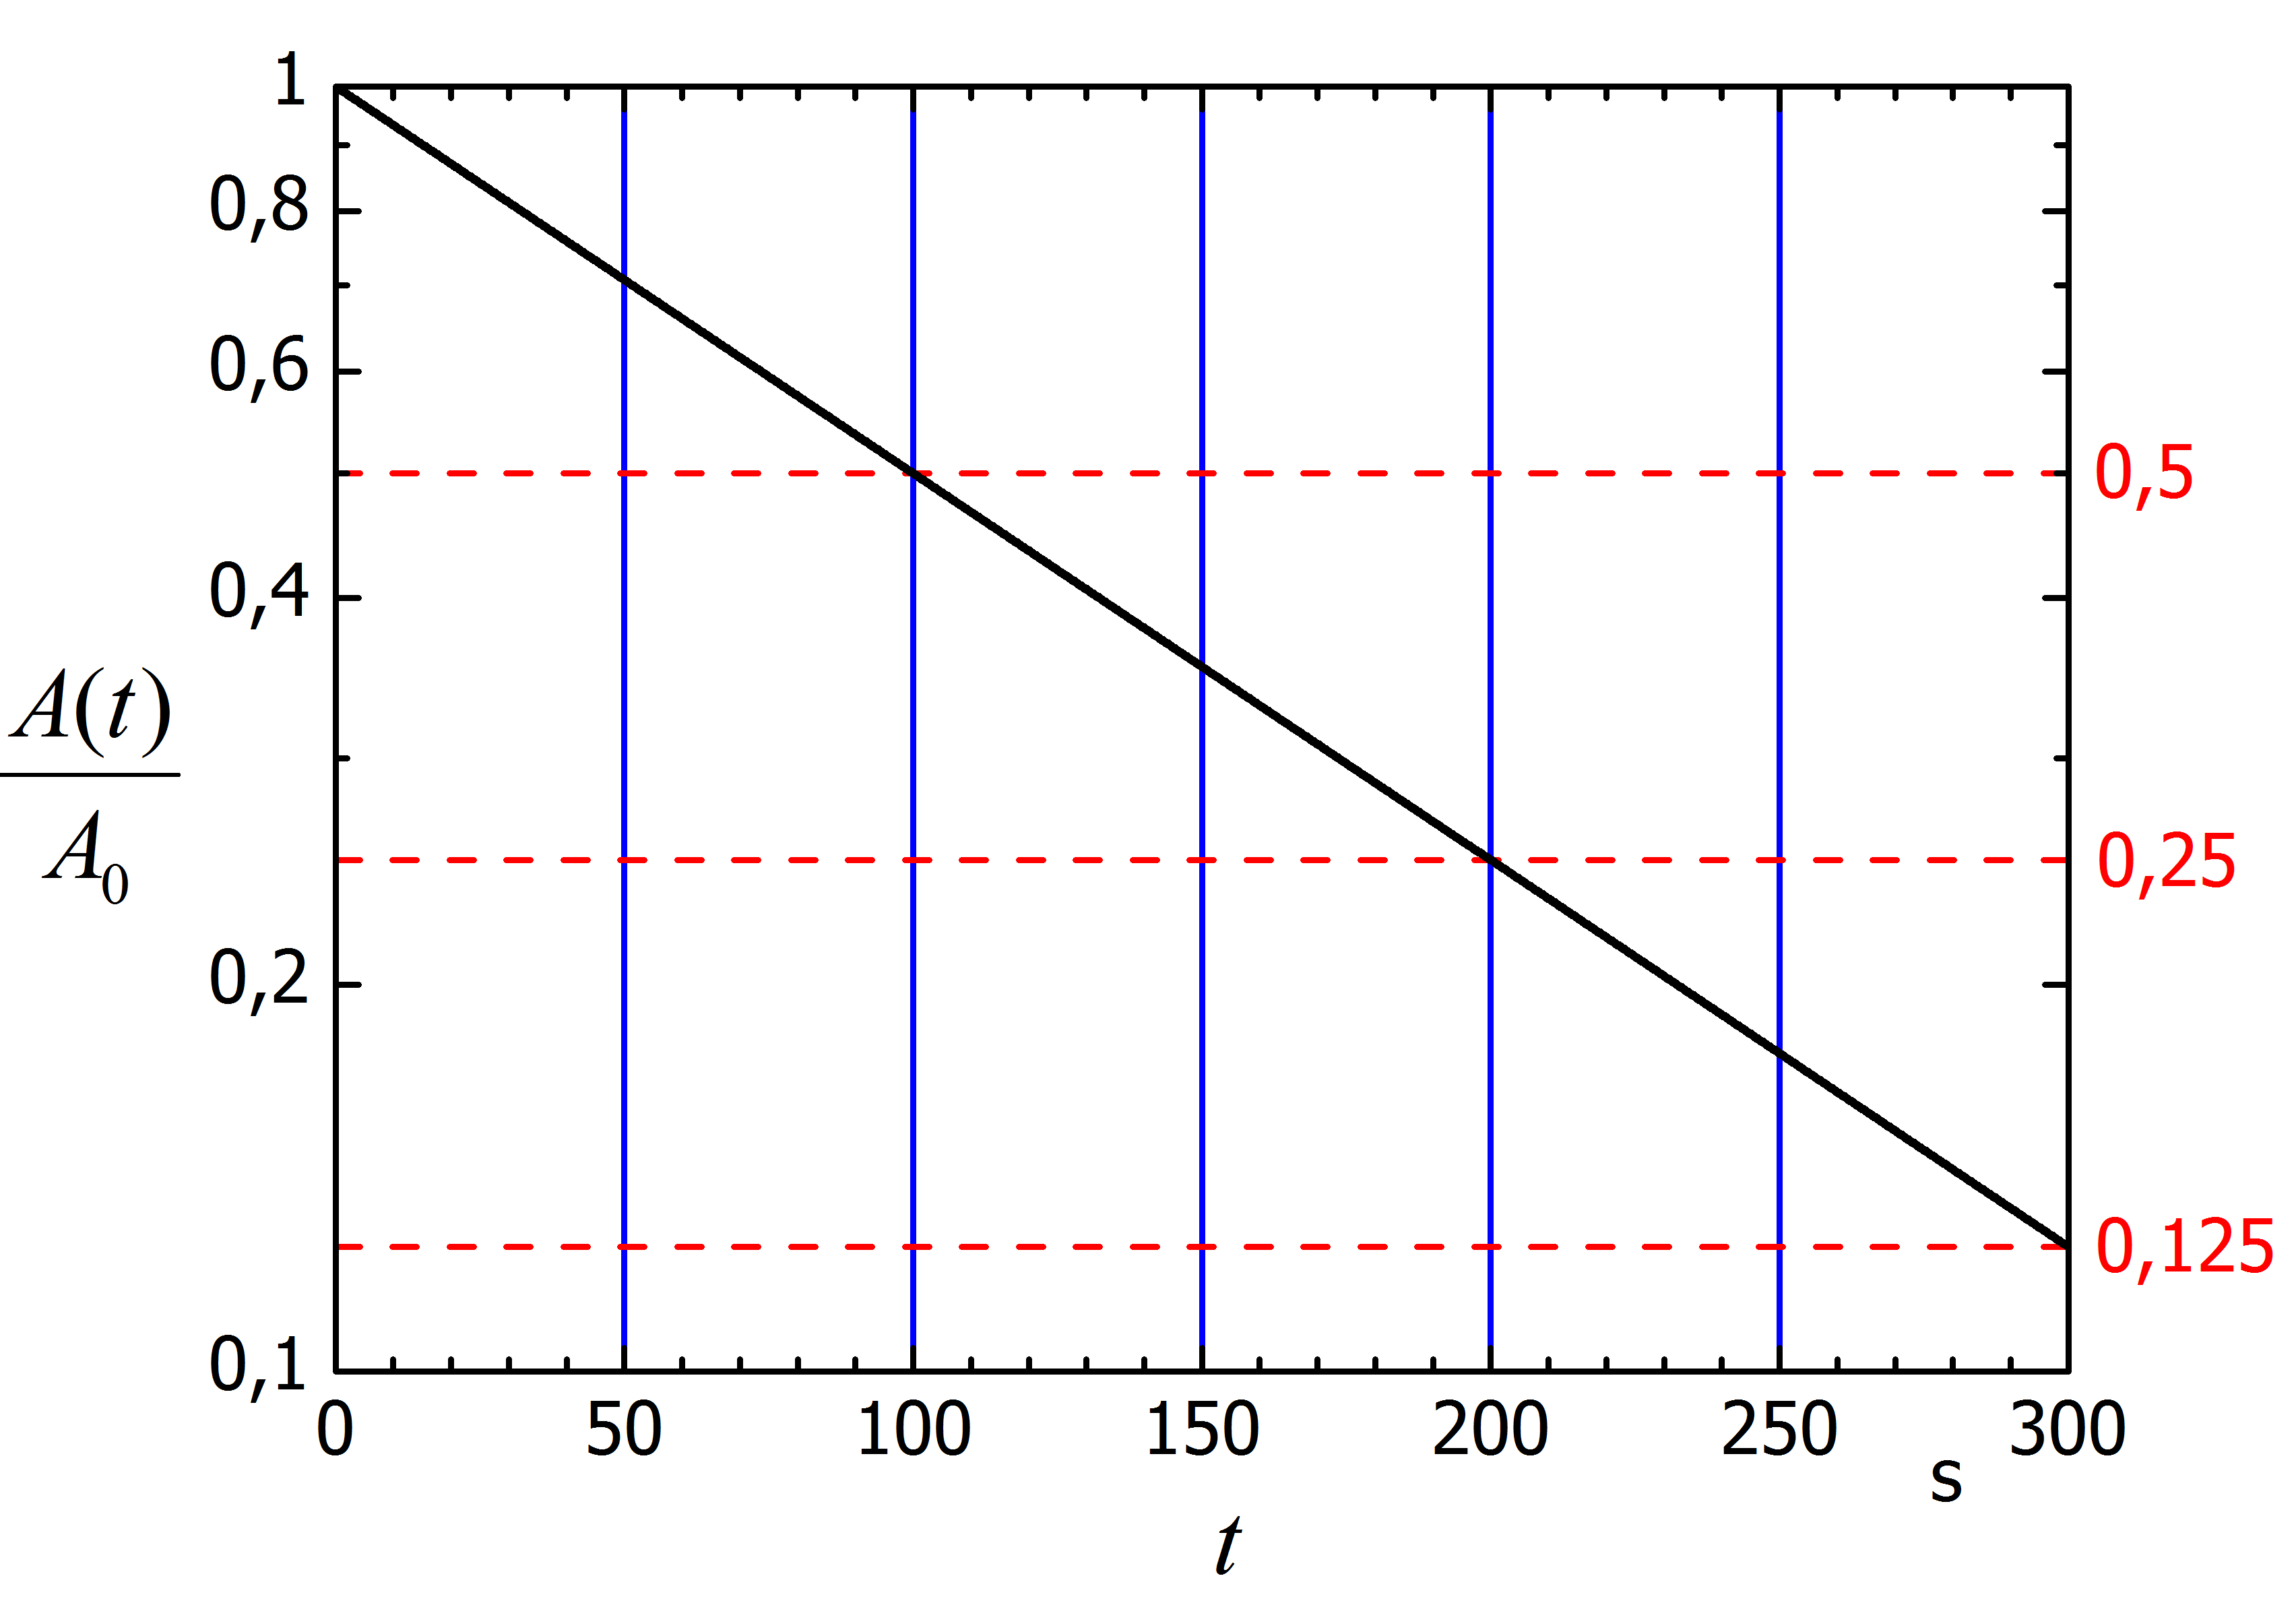
\includegraphics[width=0.6\textwidth]{Umwandlungsgesetz.png}
\caption{Plot of the decay of a nucleus with a half-life period $T_{1/2}=100$ \textsf{s}} \label{abb_umwandlungskurve}
\end{center}
\end{figure}

As an example, the progress of decay of a radionuclide with a half-life period of 100 \textsf{s} is shown in Fig. \ref{abb_umwandlungskurve}. The ratio $\nicefrac{A(t)}{A_0}$ corresponds to the fraction of initial activity after passing a period $T$. A line results in the semi-logarithmic plot. Only half of the nuclei exist after passing the half-life period. Only $\nicefrac{1}{1024}$, less than a per mille, of the initial activity could be detected after passing ten half-life periods, a little bit more than a quarter of an hour.\\


\subsection{The radionuclide $^{40}$\textsf{K}}

The radionuclide used in this experiment is $^{40}$\textsf{K} (potassium). Its contribution is $0.012~\%$ in natural potassium. In this experiment it is bound in the salt potassium carbonate \textsf{K}$_2$\textsf{CO}$_3$, which is available in a 4-molar aqueous solution. With a half-life period of $T_{1/2} = 1.27\cdot 10^9$~\textsf{a} it can be assigned to the primordial nuclides, which existed long before the creation of earth. Together with 30 other nuclides (for instance $^{87}$\textsf{Rb}, $^{176}$\textsf{Lu}, $^{187}$\textsf{Re}) it belongs to the isolated occurring, natural, primordial radionuclides. Therefore it doesn't originate from decay chains of $^{238}$\textsf{U}, $^{235}$\textsf{U}, $^{232}$\textsf{Th} or $^{237}$\textsf{Np}.\\[0,3cm]

$^{40}$\textsf{K} transmutes via $\beta^-$-decay into $^{40}$\textsf{Ca} with a probability of $89,28~\%$, as one can see in the Fig.\ref{abb_zerfallsschema}. The emitted $\beta^-$-radiation has a maximum energy of 1,31 \textsf{MeV}. $^{40}$\textsf{K} transmutes to $^{40}$\textsf{Ar} via electron capture at a probability of $10,72~\%$. The transmutation into the ground state of $^{40}$\textsf{Ar} only occurs in $0,048~\%$ of all $^{40}$\textsf{K} nuclides. $10,67~\%$ first transmute into an excited state of $^{40}$\textsf{Ar}, which decays into the ground state by emitting $\gamma$-radiation of an energy of 1,46 \textsf{MeV}. \\[0,3cm]

\begin{figure}[htbp]
\begin{center}
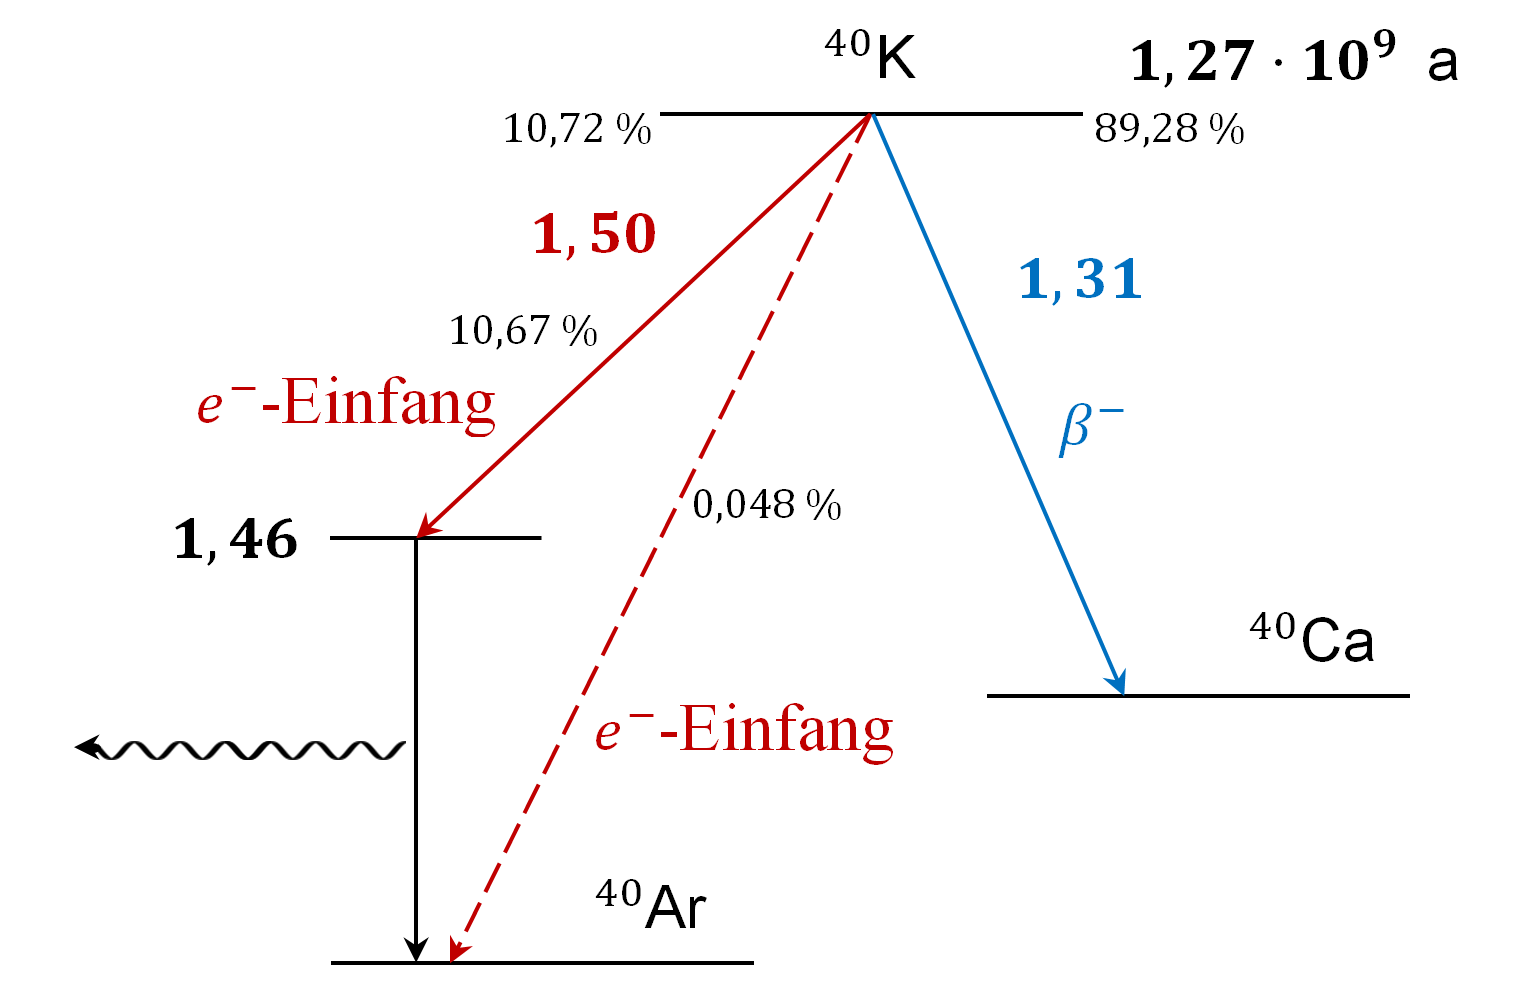
\includegraphics[width=0.6\textwidth]{Zerfallsschema-K-40.png}
\caption{Decay scheme for the radionuclide $^{40}$\textsf{K}. (Energy levels and notation in \textsf{MeV})} \label{abb_zerfallsschema}
\end{center}
\end{figure}


\subsection{Statistics of counting measurements}

A measurement of a radioactive decay will be done by \textit{counting measurements} of the emitted radiation. That is valid for so-called basic as well as spectrometric and/or coincident counting measurements. The first method simply counts events, while the latter two methods only consider events matching certain defined additional criteria like matching a certain energy range or time window.\\[0,3cm]
The immediate result of a counting measurement is a certain number of counted events $x$ (at electronic measurements: counting impulses), which were acquired during a certain time period, the \textit{measurement time}~$t_\mathrm m$. The resulting \textit{counting rate}
 
\begin{eqnarray}
Z &=& \frac{x}{t_\mathrm m} \label{glg_zaehlrate}
\end{eqnarray}
is a dimension of the intensity or flux density of the measured radiation. 
The counting rate is known at the efficiency $\eta_Z$ due to the relation $Z=\eta_Z \cdot A$. It is also a dimention of the measured activity $A$.\\[0,3cm]

All counting measurements obey certain statistical laws, which a priori lead to statistical fluctuations of the measurement values (in this case the number of measured counting impulses).
It is for measurements of the radioactive decay that the process of decay itself is a stochastic process. The used experimental devices acquire in the rarest cases $100~\%$ of the radiation. For instance, indirectly ionizing kinds of radiation (photons and neutrons) can pass the detector without any interaction and can therefore not be acquired.\\ [0,3cm]
In the following sections only the the statistical fluctuations of the radioactive decays for a given time interval will be discussed. If the probability for the acquisition of a decay event with a corresponding measurement device is constant $~-~$ which normally can be supposed $~-~$ then the discussed laws apply also to the corresponding measurements.\\[0,3cm]
Discrete statistical distributions are described by the probability function $P(x)$ in the theory. Continuous distributions are described by the (probability) density function $f(x)$. Both functions are normalized to 1 by definition. 

The \textit{mean} $\mu$ and the \textit{variance} $\sigma ^2$ are defined as:

\begin{eqnarray}
\mu ~~=~~ \sum\limits _x {x\cdot P(x)} ~~~~~~~~~~~~~~~~~~~~~~~~~~~~~~~~ \mu &=& \int\limits_{- \infty}^{+ \infty}{x\cdot f(x) \mathrm dx}  \label{glg_mittelwert} \\
\sigma ^2 ~~=~~ \sum\limits _x {(x-\mu)^2\cdot P(x)}~~~~~~~~~~~~~~~~~~~~~~ \sigma ^2 &=& \int\limits_{-\infty}^{+\infty}{(x-\mu)^2\cdot f(x) \mathrm dx} \label{glg_standardabweichung}
\end{eqnarray}

\subsubsection{Binomial distribution}

The probability of a transmutation of a \textit{single} nucleus in the time period $t$ is described by the exponential law of decay (\ref{glg_umwandlungsgesetz}) as:

\begin{eqnarray}
p &=& 1 - \mathrm e^{-\lambda \cdot t}
\end{eqnarray}
 
Generally the decay of a single nucleus in not of interest. Therefore, a certain number, $N$, of radioactive nuclei (the \textit{basic population}) is always treated. Because decays are independent to each other, more decays can occur during a time period $t$. However, a transmuted nucleus can't decay again in the same way. It is excluded from future processes. Under consideration of these circumstances the probability $P(x)$ of the occurrence of exactly $x$ random events can be expressed by the \textit{binomial distribution} as:
\begin{eqnarray}
P(x) &=& {N \choose x}\cdot p^x \cdot (1-p)^{N-x} ~~=~~ {N \choose x} \cdot (1 - \mathrm e^{-\lambda \cdot t})^x \cdot (\mathrm e^{-\lambda \cdot t})^{N-x} \label{glg_binomialverteilung}
\end{eqnarray}
The mean value follows
\begin{eqnarray}
\mu &=& N \cdot p ~~=~~ N\cdot (1 - \mathrm e^{-\lambda \cdot t}) \label{glg_bin_mittelwert}
\end{eqnarray}
and the variance can be determined as:
\begin{eqnarray}
\sigma ^2 &=& N \cdot p \cdot (1-p) ~~=~~ N \cdot(1 - \mathrm e^{-\lambda \cdot t}) \cdot \mathrm e^{-\lambda \cdot t} \label{glg_bin_standardabweichung}
\end{eqnarray} 

This distribution function is valid for the statistics of all decay processes with a fix non-influenceable decay constant $\lambda$. Even more generally expressed, it is a matter of so called 
\eigen{Bernoulli}\textit{-experiments}, where only two different excluding events with a constant probability can occur. 

\subsubsection{\eigen{Poisson}-distribution}
The binomial distribution results the exact solution for the statistics of the radioactive decay. 
In the case of treating only a small number $N$ of nuclei, one has to calculate according to binomial distributions. For relatively small $N$ the calculation of the binomial coefficients is not difficult. For big $N$ it is not so easy anymore, because of the very big values in the factorial.
Exactly for this case and for small observation times compared to the half-life period one has

\begin{eqnarray}
\lambda \cdot t &=& \frac{\ln 2 \cdot t}{T_{1/2}} ~~\ll ~~ 1 ~~~\mathrm{and}~~~ x ~~\ll ~~ N \label{glg_poi_bed}
\end{eqnarray}
and the binomial distribution transforms into the \eigen{Poisson}\textit{-distribution}
\begin{eqnarray}
P(X=x) &=& \frac{(N\cdot p)^x}{x!} \cdot \mathrm e^{-N\cdot p} ~~=~~ \frac{\mu ^x}{x!}\cdot \mathrm e^{- \mu} ~~~~.\label{glg_poisson}
\end{eqnarray}
It describes the distribution of very rare events, which occur with a small but constant probability $p = 1 - \mathrm e^{- \lambda \cdot t}$ amongst a very big number of \grqq subjects \grqq~$N$$~-~$ in this case the sum of the considered radioactive nuclei. Any further observations of the number $N$ of radioactive nuclei is obsolete by the transition $N \cdot p ~\rightarrow ~ \mu$ and only the expectation value for the discrete random value ~$X$ is of interest. 
The expectation value is equal to the variance $\sigma ^2$ resp. the standard deviation one has: $\sigma = \sqrt{\mu}$. Therefore the \eigen{Poisson}-distribution has only one distribution parameter ~$\mu$.\\[0,3cm]
The relation (\ref{glg_poisson}) can be easily evaluated by using computational tools. 
A \textit{recursive formula} 
\begin{eqnarray}
P(x) &=& \frac{\mu}{x} \cdot P(x-1) \label{glg_poi_rek}
\end{eqnarray}
begins at the initial link $P(0) = \mathrm e^{-\mu}$. Only bar charts or the like are valid for plotting the probability function of discrete distributions (see for instance Fig.\ref{abb_pois_1}). Connections of the values to a closed curve is of course forbidden by the discrete domain of definition. 

\begin{figure}[htbp]
\begin{center}
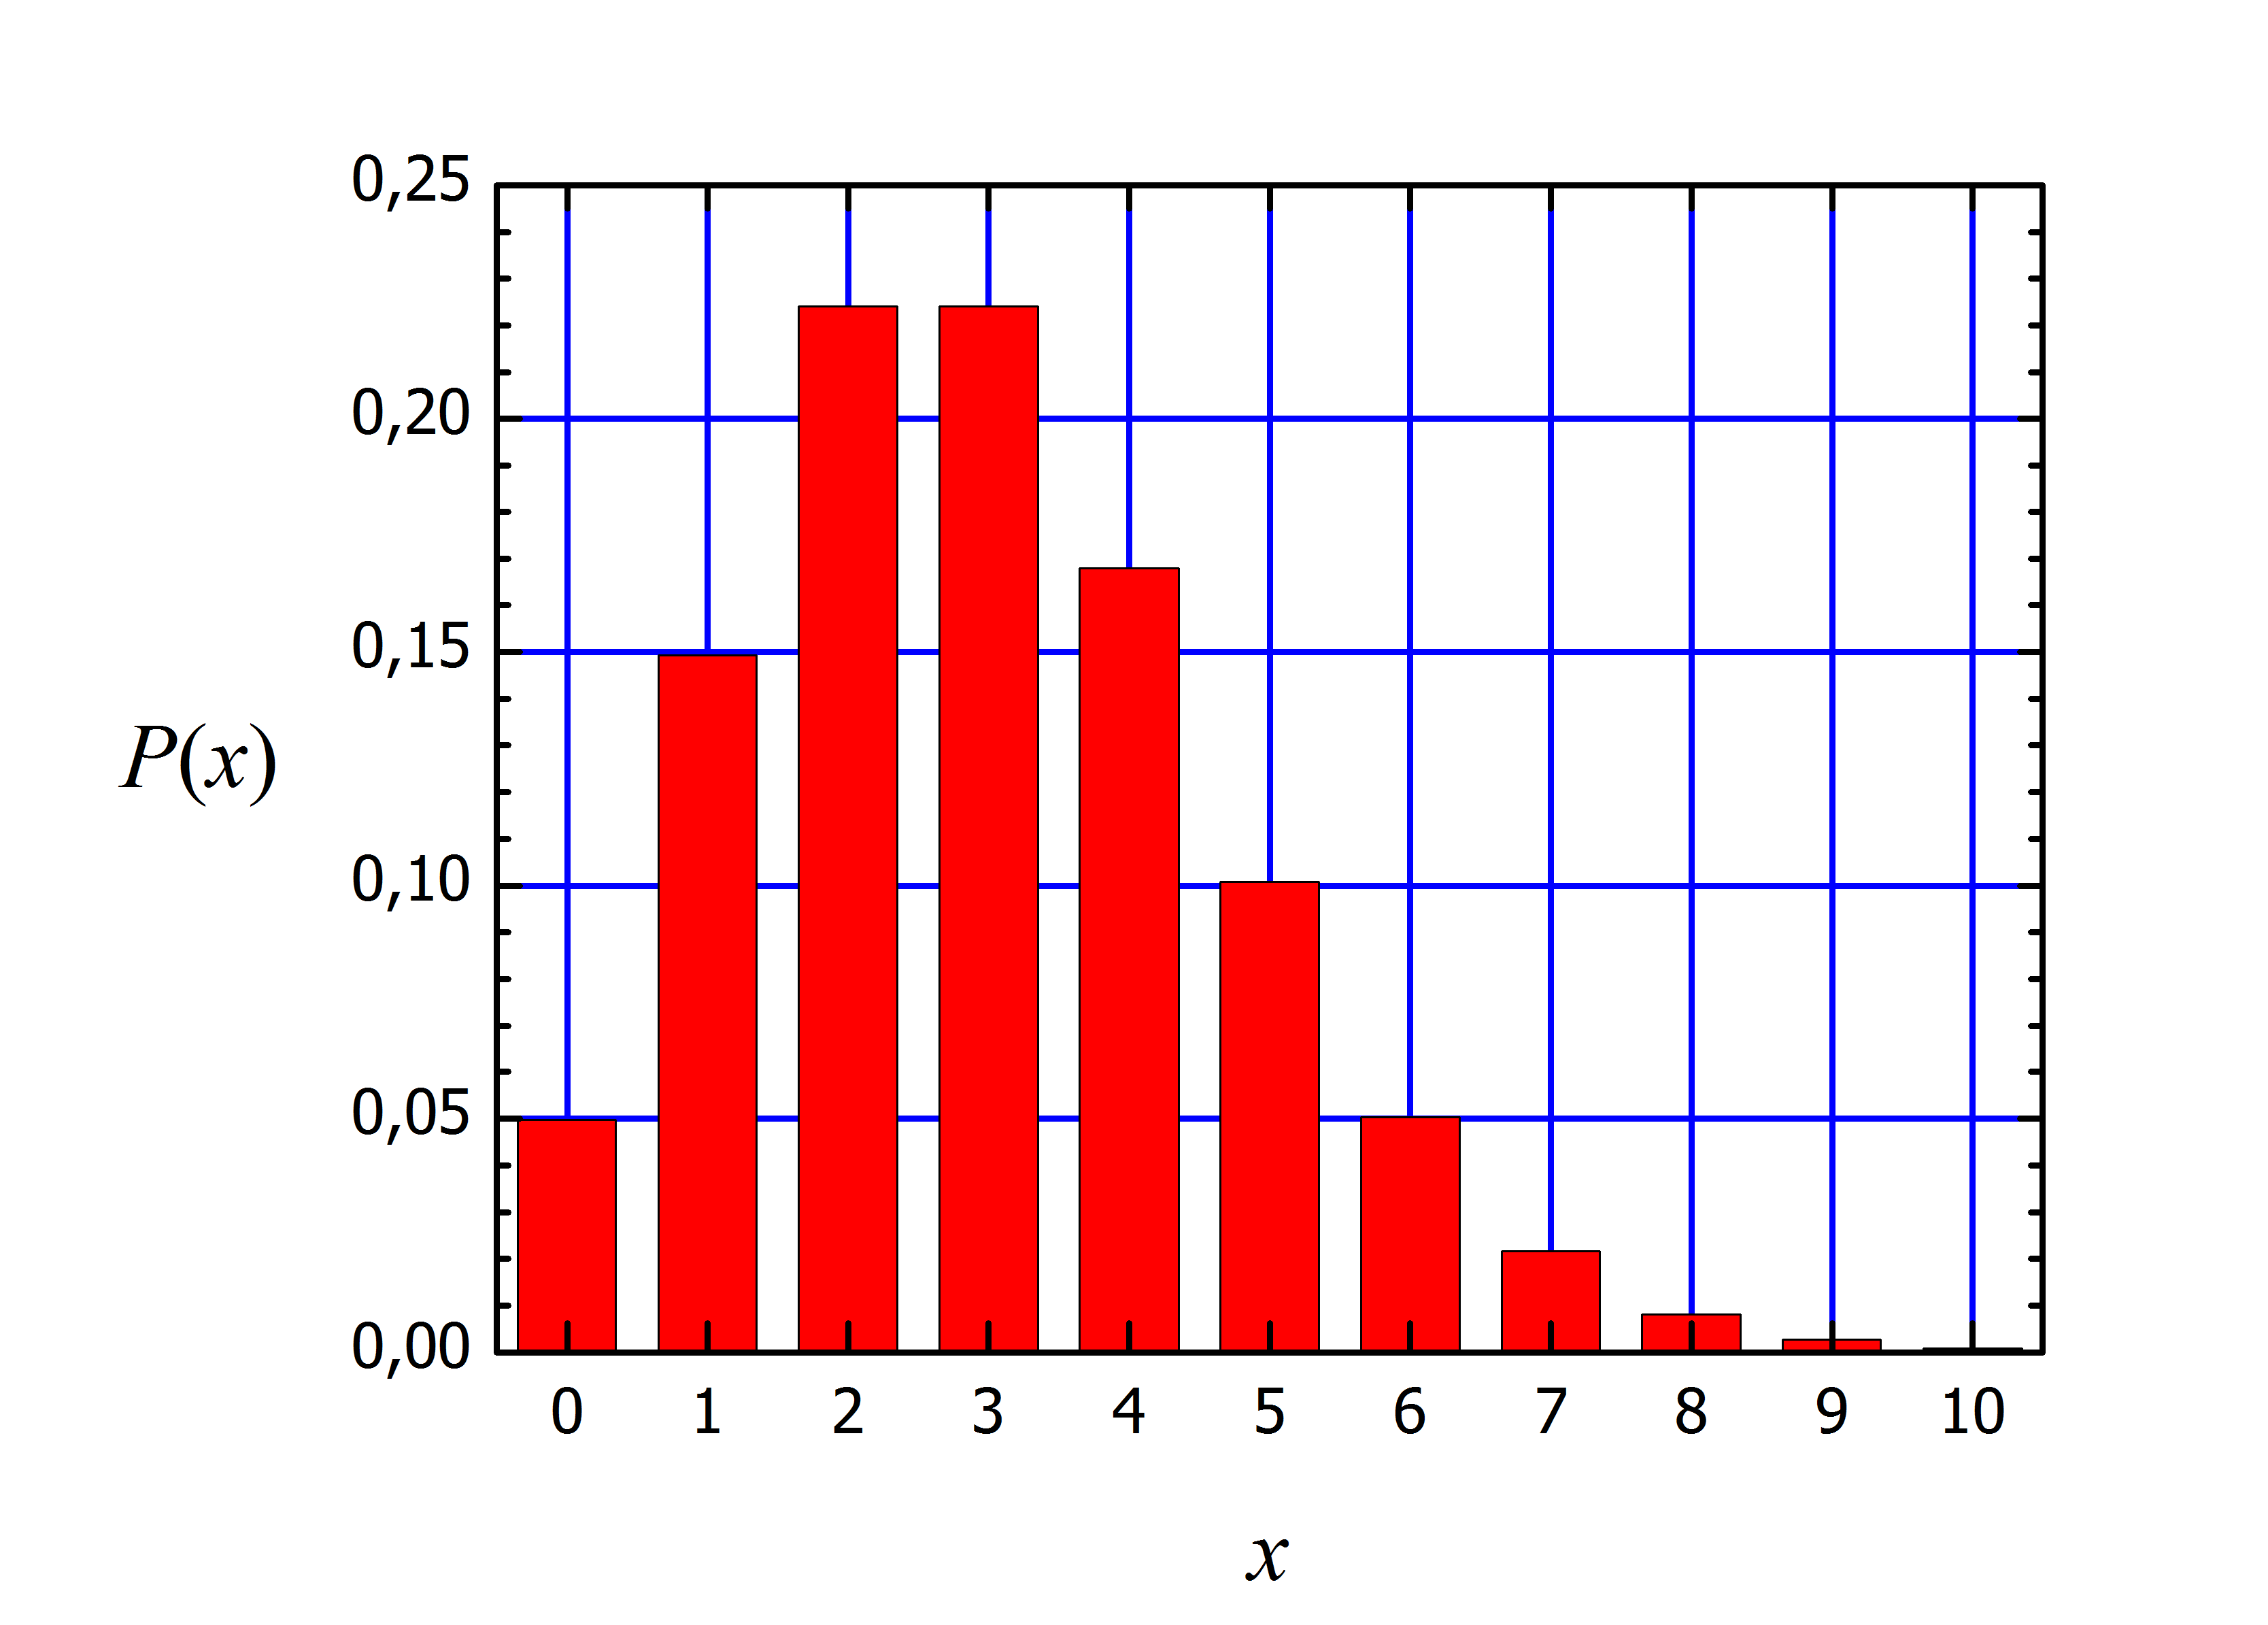
\includegraphics[width=0.6\textwidth]{Poisson-mu-3.png}
\caption{Probability function $P(X=x)$ of a \eigen{Poisson}-distributed random variable $X$ with $\mu = 3$} \label{abb_pois_1}
\end{center}
\end{figure}
In most real-life-cases the conditions of (\ref{glg_poi_bed}) are fulfilled. The \eigen{Poisson}-distribution is therefore the correct approach for a statistical description of the radioactive decay. Anyway there are some restrictions for practical applications: The calculations according to (\ref{glg_poisson}) becomes inaccurate for big $\mu$. Also, the application of statistical tests to verify the so-called \textit{purity} of the distribution is difficult. A transition to the continuous \eigen{Gaussian}-\textit{distribution} is useful for this purpose. 


\subsubsection{\eigen{Gaussian}-/Normal distribution}

Using the Stirling formula for calculating the factorial of big numbers as well as transitioning to a continuous random variable follows for counting measurements the density function
\begin{eqnarray}
f(x) &=& \frac{1}{\sqrt{2\pi \cdot \mu}}\cdot \mathrm e^{-\frac{(x-\mu)^2}{2\mu}} ~~~~~, \label{glg_gauss_1}
\end{eqnarray}
which is a special expression of the density function
\begin{eqnarray}
f(x) &=& \frac{1}{\sqrt{2\pi}\cdot \sigma} \cdot \mathrm e^{-\frac{1}{2}\cdot \left( \frac{x-\mu}{\sigma} \right)^2} \label{glg_gauss_0}
\end{eqnarray}
the \eigen{Gaussian}-\textit{distribution}. (\ref{glg_gauss_1}) has, in opposite to (\ref{glg_gauss_0}), only one distribution parameter, because the variance $\sigma ^2$ coincides with the expectation value $\mu$. The normal distribution with the density function (\ref{glg_gauss_1}) is the limiting case for the \eigen{Poisson}-distribution at big expectation values. The approach to the discrete \eigen{Poisson}-distribution with a continuous \eigen{Gaussian}-distribution is always just a approximation, even though for $\mu > 10$ it is a useful approximation and for $\mu > 50$ it is a relatively accurate approximation. That has always to be considered in direct comparisons of counting measurements to this theoretical distribution function.  

\subsubsection{Theoretical and empirical distribution functions}

The \textit{theoretical} distribution function $F(x)$ for a discrete random variable is defined as: 
\begin{eqnarray}
F(X \leq x) = \sum\limits_{i=0}^{x}{P(X=i)} \label{glg_verteilungsfunktion_dis}
\end{eqnarray}
The definition for a continuous random variable is:
\begin{eqnarray}
F(X \leq x) &=& \int\limits_{- \infty}^{x}{f(x')\mathrm dx'} \label{glg_verteilungsfunktion_stet}
\end{eqnarray}
 Because of the normalization of the density resp. probability function it is always \linebreak $F(-\infty) = 0$ and $F(\infty)=1$. It is $F(a) = P(x=a)$ and $F(b)=1$, if $f(x)$ resp. $P(x)$ are defined only on an interval $[a,~b]$ .\\[0,3cm]

The distribution functions can be expressed as:
\begin{eqnarray}
F(X\leq x) ~~=~~ N(x) &=& \frac{1}{\sqrt{2\pi \cdot \mu}}\cdot \int\limits_{-\infty}^{x}{\mathrm e^{-\frac{(x'-\mu)^2}{2\mu}}\mathrm dx'} \label{glg_vert_gauss_1}
\end{eqnarray}

That is the theoretical distribution function to (\ref{glg_gauss_1}), which is analytically not solvable.\\[0,3cm]
The expectation value $\mu$ is de facto unknown. Therefore it has to be estimated during the measurements. For that, a series of $n$ single measurements will be performed. The measurement values $x_i$ during the counting measurements can only result in values of natural numbers.
The mean value
\begin{eqnarray}
\overline x &=& \frac{1}{n} \cdot \sum\limits_{i=1}^{n}{x_i} \label{glg_mittelwert_2}
\end{eqnarray}
is a positive rational number and an estimated value for the theoretical expectation value $\mu$.
It is also designated as the \textit{statistical} or \textit{empirical} expectation value $\mu_x$.
A suitable dimension for the fluctuation of the single measurements is the \textit{empirical standard deviation} $\sigma_x$ of the measurement series, which results from the variance:

\begin{eqnarray}
\sigma_x^2 &\approx & \frac{1}{n-1}\cdot \sum\limits_{i=1}^{n}{(x_i - \overline x)^2}
\end{eqnarray}

For the computional evaluation the expression 
\begin{eqnarray}
\sigma_x^2 ~~\approx ~~ \frac{1}{n-1}\cdot \left( \sum\limits_{i=1}^{n}{x_i^2 - n\cdot \overline{x}^2} \right) &=& \frac{n}{n-1}\cdot \left( \overline{x^2} - \overline{x}^2 \right) ~~\stackrel{(\mathrm{f"ur~gro"se~}n)}{\approx}~~ \overline{x^2} - \overline{x}^2 \nonumber
\end{eqnarray}
is useful. Another important dimension is the \textit{standard deviation of the mean value} $\sigma_{\overline x}$, which results from the corresponding variance:
\begin{eqnarray}
\sigma^2_{\overline x} &=& \frac{\sigma^2_x}{n} ~~\approx ~~ \frac{1}{n(n-1)}\cdot \left( \sum\limits_{i=1}^{n}{x_i^2 - n\cdot \overline x^2} \right) ~~~~~. \label{glg_mw_stdabw}
\end{eqnarray}

The statistical evaluation of measurement series via (\ref{glg_mittelwert_2}) - (\ref{glg_mw_stdabw}) is not an exception of counting measurements, but also valid for continuous distributions (see manual of the experiment "`error analysis"'). 
In our case the measurement series are normally distributed and follow (\ref{glg_gauss_0}) and (\ref{glg_vert_gauss_1}).\\[0,3cm]
The statistics of the counting measurement obey a \eigen{Poisson}-distribution.
As mentioned before, the theoretical value of the variance $\sigma^2$ coincide with the expectation value $\mu$. The theoretical standard deviation is therefore always $\sigma = \sqrt{\mu}$. \\[0,3cm] 

A single measurement ($n=1$) of $N$ impulses already provides a random sample of the expectation value $(\mu \approx N)$. Thus the variance $\sigma^2 \approx N$ and the standard deviation $\sigma \approx \sqrt{N}$ can be estimated as well as the relative standard deviation $\varepsilon_\sigma \approx \nicefrac{1}{\sqrt{N}}$. Therefore it isn't important if the $N$ impulses are acquired at once or in a series of $k$ sub-measurements and accumulated according to: 
\begin{eqnarray}
N &=& \sum\limits_{i=1}^{k}{x_i} \label{glg_gesamtanzahl}
\end{eqnarray}
The only restriction is that this is again only a statistical estimation and it obeys the \eigen{Poisson}-statistics.\\[0,3cm]

The mean value $\overline x = \nicefrac{N}{n}$ according to (\ref{glg_mittelwert_2}) is the estimation of the empirical expectation value $\mu_x$ of a single measurement. The theoretical standard deviation is $\sigma = \sqrt{\overline x}=\sqrt{\nicefrac{N}{n}}$ for a population of $n$ equal single measurements with a total number of impulses $N$.
The \textit{relative rate function} $h(X=x) = \frac{H(X=x)}{n}$ is the empirical probability function, where $H(x)$ is the absolute rate of events of the kind $X=x$.\\[0,3cm]

Fig. \ref{abb_pois_vs_gauss_a} shows the \eigen{Gau�}-approximation of a large number of random samples from a \eigen{Poisson}-distribution. Both distributions have a standard deviation of $\sigma = \sqrt{\mu} = \sqrt{49} = 7$. The asymmetry of the \eigen{Poisson}-distribution is also obvious at this big expectation value. The plot of the very small uncertainties is waived, because of the big number of random samples 
\begin{figure}[htbp]
\begin{center}
\subfigure[Empirical rate function \label{abb_pois_vs_gauss_a}]
{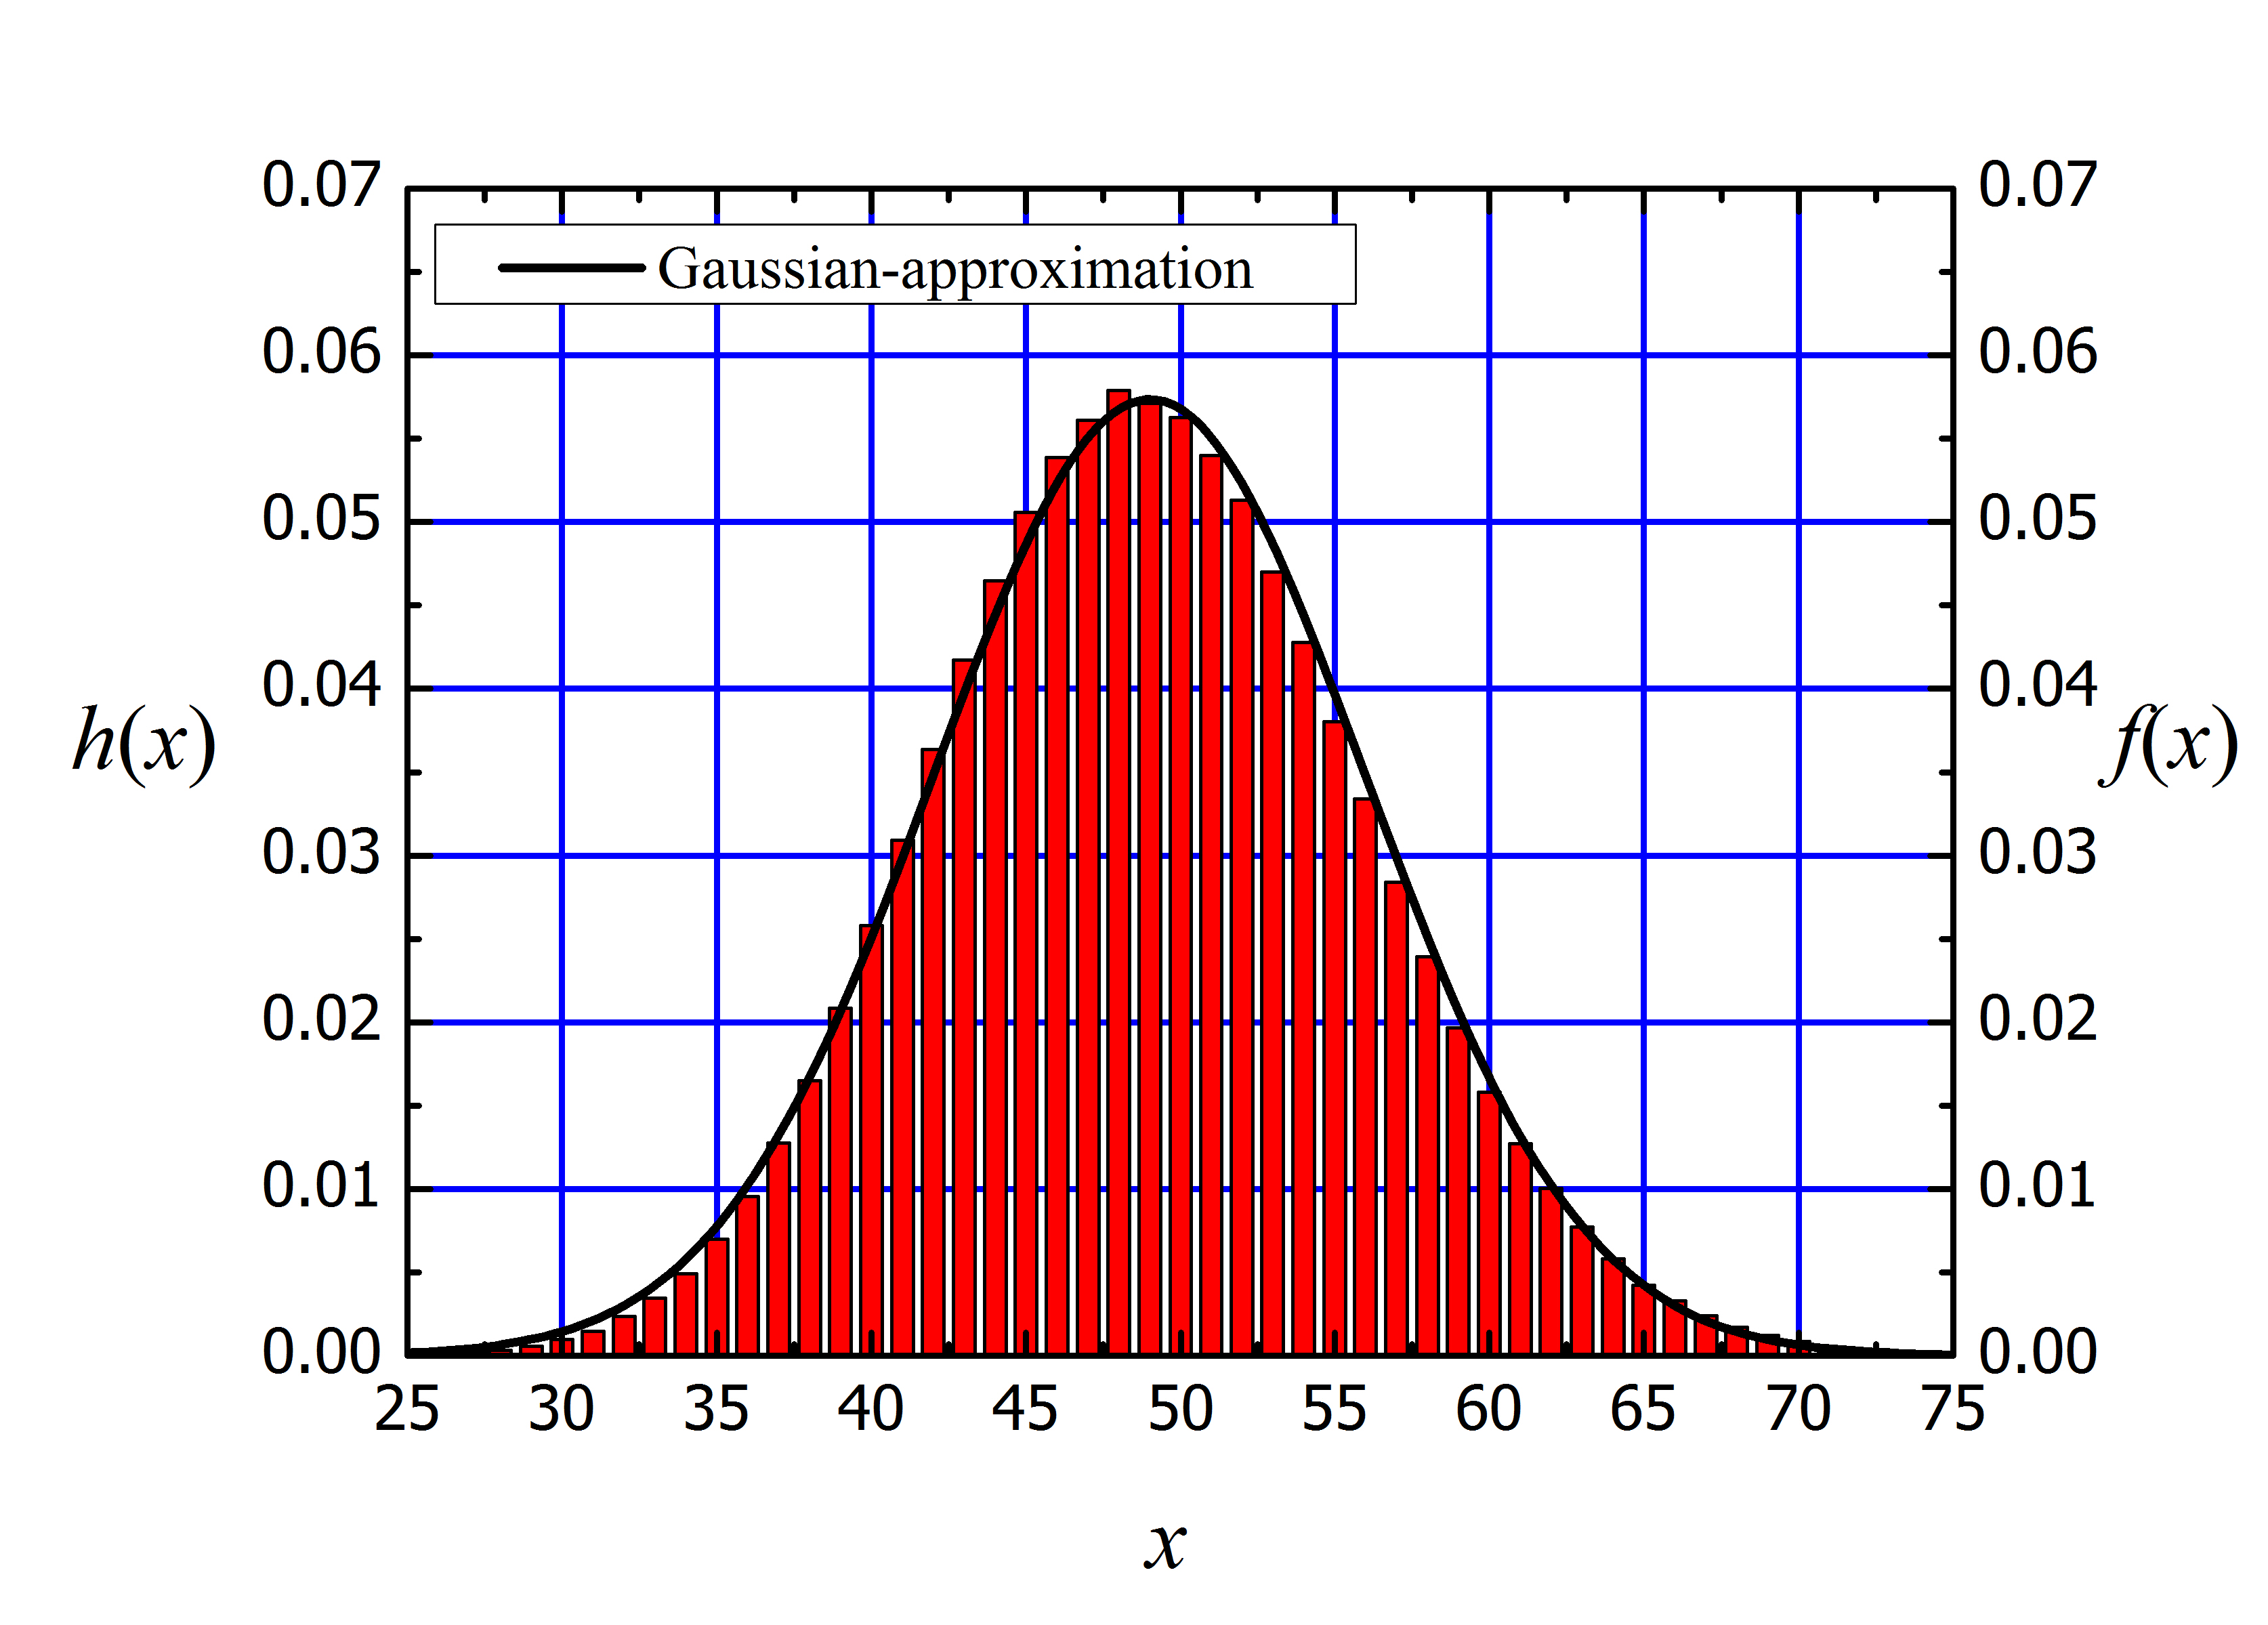
\includegraphics[width=0.6\textwidth]{Poisson-Gauss-mu-49.jpg}}
\subfigure[relative cumulative rate \label{abb_pois_vs_gauss_b}]
{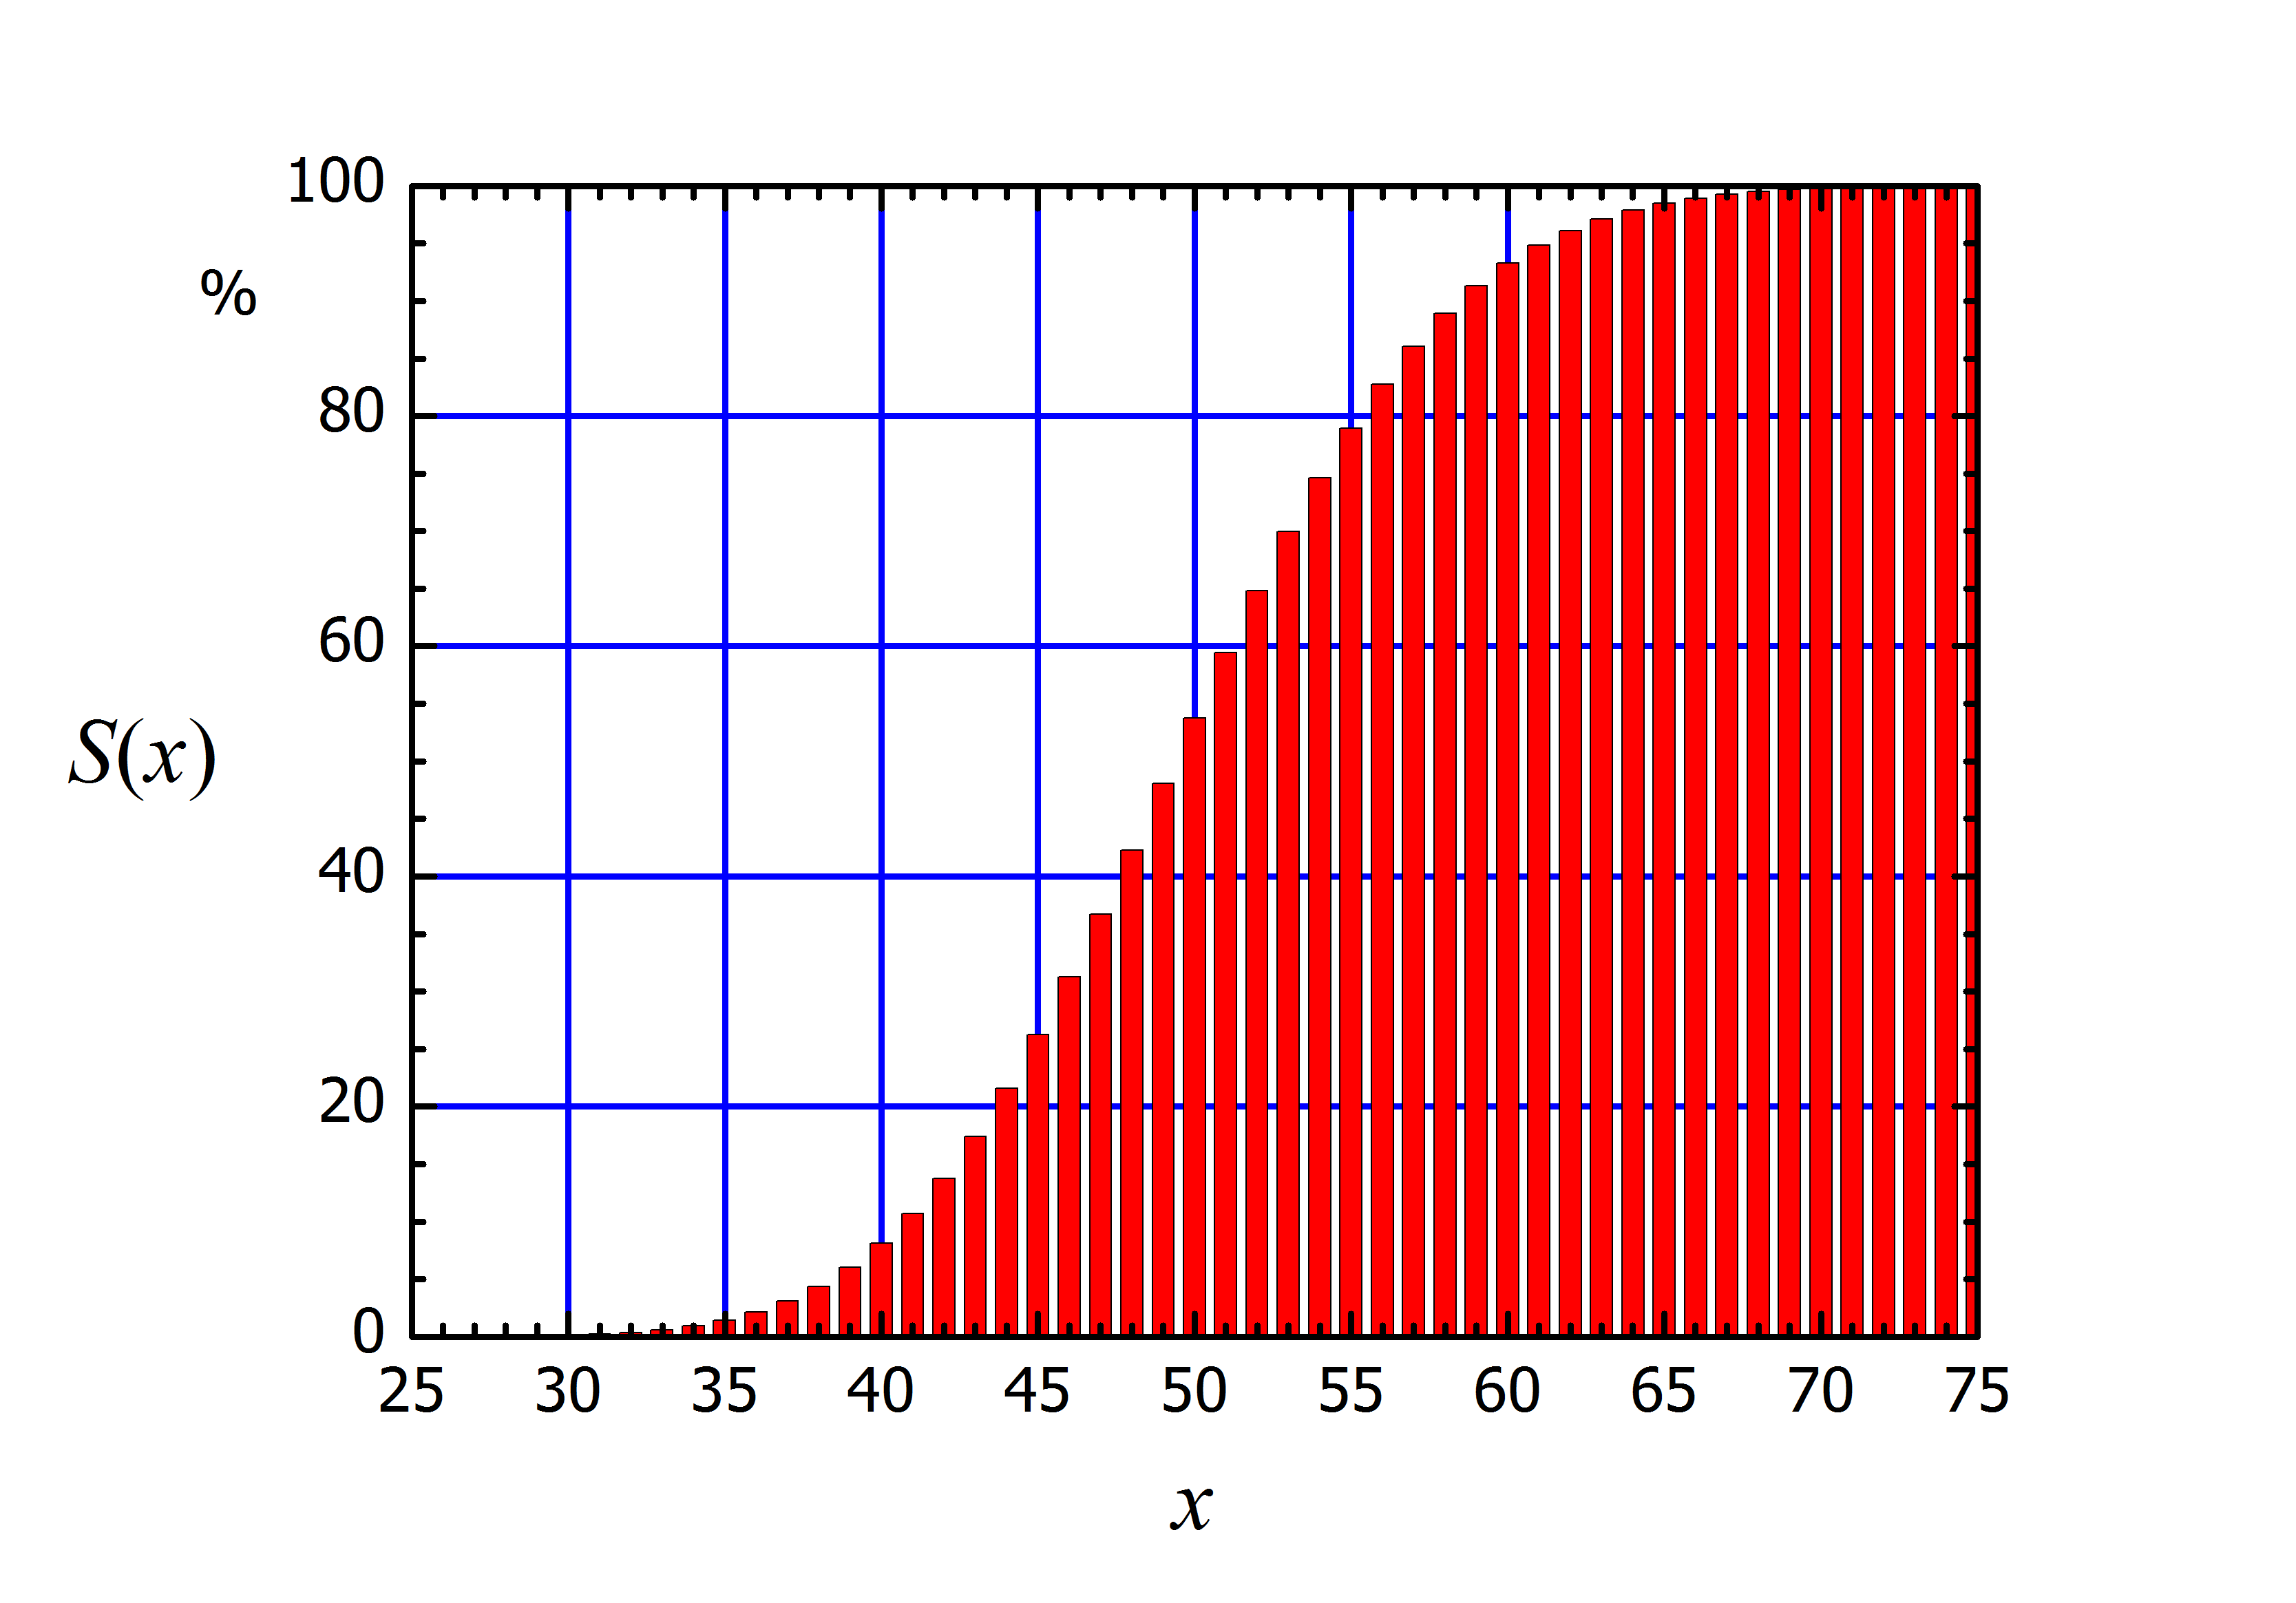
\includegraphics[width=0.6\textwidth]{Poisson-mu-49-sum-hfkt}}
\subfigure[Empirical distribution function in comparison to the theoretical distribution function \label{abb_pois_vs_gauss_c}]
{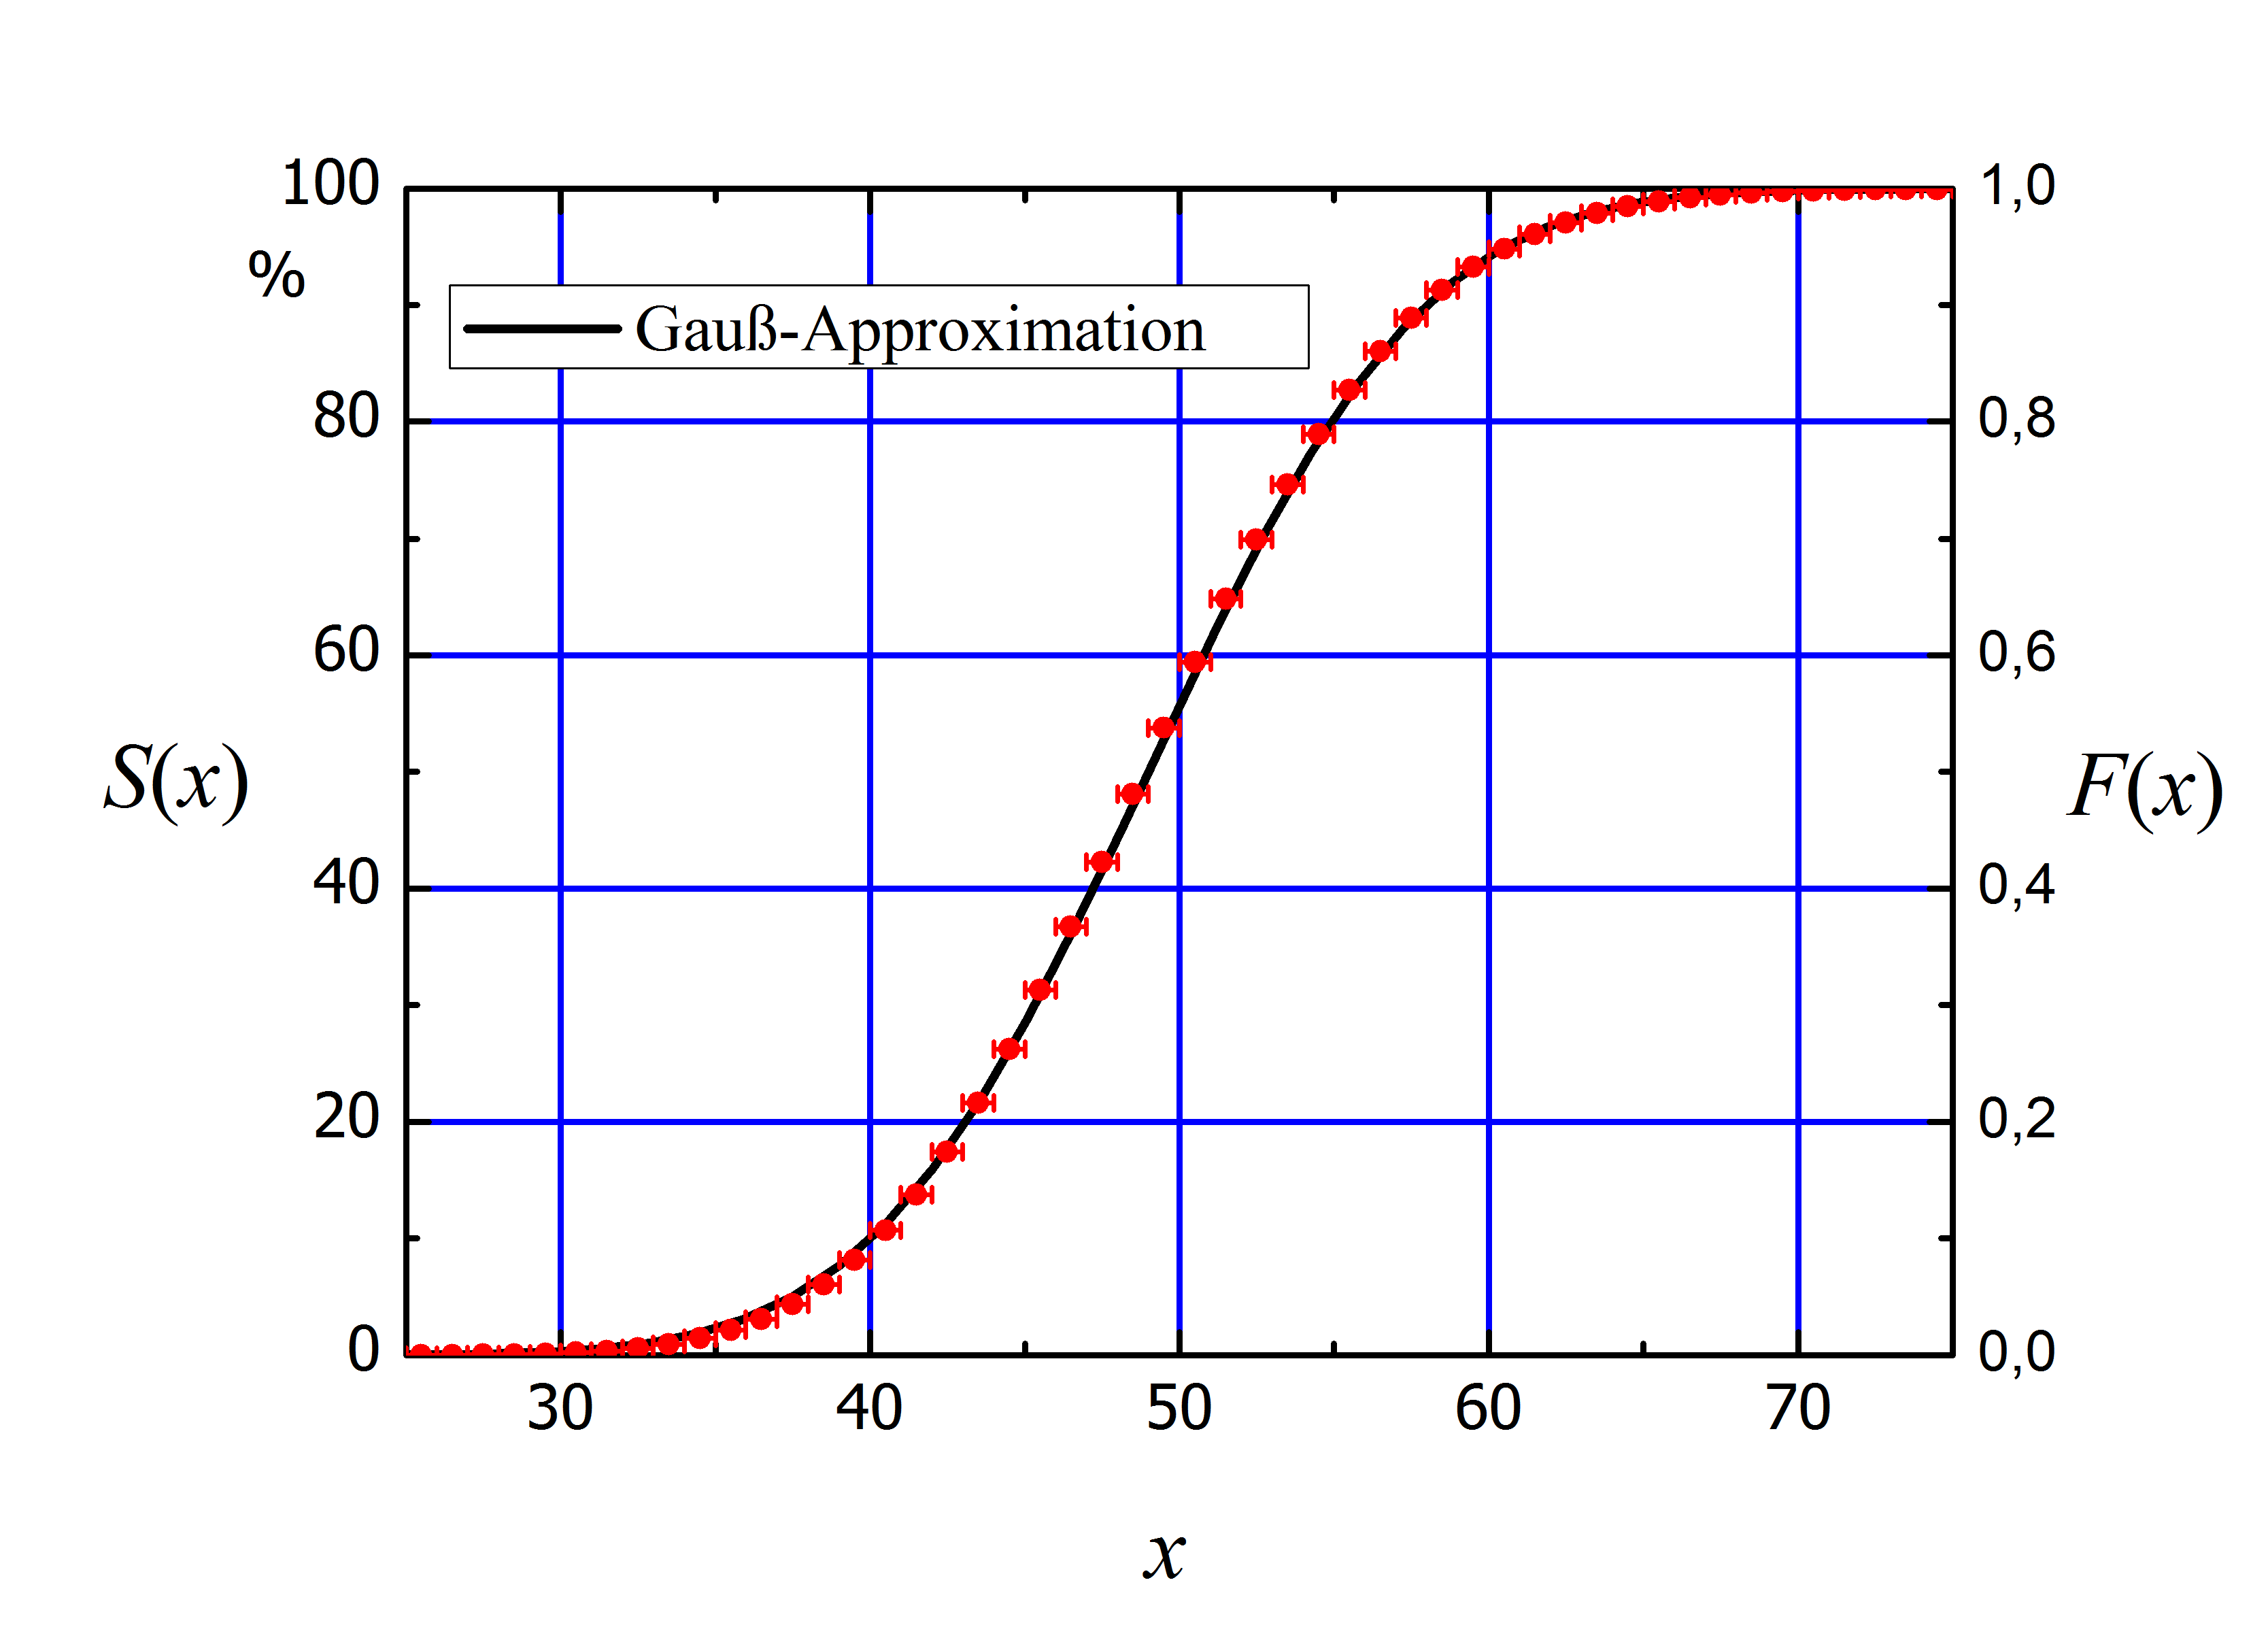
\includegraphics[width=0.6\textwidth]{Poisson-Gauss-mu-49-sum-hfkt}}
\caption{$n=10^6$ random samples from a \eigen{Poisson}-distribution with the expectation value of $\mu = 49$ in comparison to the density function of the \eigen{Gaussian}-distribution} \label{abb_pois_vs_gauss}
\end{center}
\end{figure}\\[0,3cm]
The \textit{empirical} distribution function can be expressed by the \textit{relative cumulative rate}
\begin{eqnarray}
S(X\leq x) &=& \sum\limits_{k=1}^{x}{h(k)} ~~=~~ \frac{1}{n}\cdot \sum\limits_{k=1}^{x}{H(k)} ~~~~~, \label{glg_sumhfkt}
\end{eqnarray}
which is mostly represent by $\%$. It is the equivalent of the theoretical distribution function $F(x)$. If the normalized cumulative rate (\ref{glg_sumhfkt}) is compared to the distribution function (\ref{glg_verteilungsfunktion_stet}), then a correction of continuity has to 
be performed for the normalized cumulative rate. This is necessary to reconnect the discrete points of a summation of $S(x)$ with the continuous limits of the integration of $F(x)$. Therefore the data points of the empirical distribution function from Fig. \ref{abb_pois_vs_gauss_b} will be entered into the corresponding end of the interval in Fig.\ref{abb_pois_vs_gauss_c}. In this example at $\tilde{x}=x+0.5$. \\[0,3cm]
Now a population of only $n=1000$ random samples, like in the experiment, will be discussed. For that a random generator generates numbers according to a \eigen{Poisson}-distribution with a set expectation value of $\mu =49$ and a standard deviation of $\sigma = 7$. The result is the rate distribution $H(x)$ of random numbers, shown in Fig.\ref{abb_pois_n_1000}.
During these 1000 random samples $N=49212$ impulses will be measured in total. This corresponds to an expectation value of $\mu_x = \overline{x} = 49.21$. For the empirical standard deviation $\sigma_x = 7.09$ will be evaluated. The observed empirical width of fluctions of the mean value is $\sigma_{\overline{x}} = 0.22$. The measured mean value was barely within the width of fluctuations of the "`true"' value of $\mu = 49$ in this "`experiment"'.

\begin{figure}[htbp]
\begin{center}
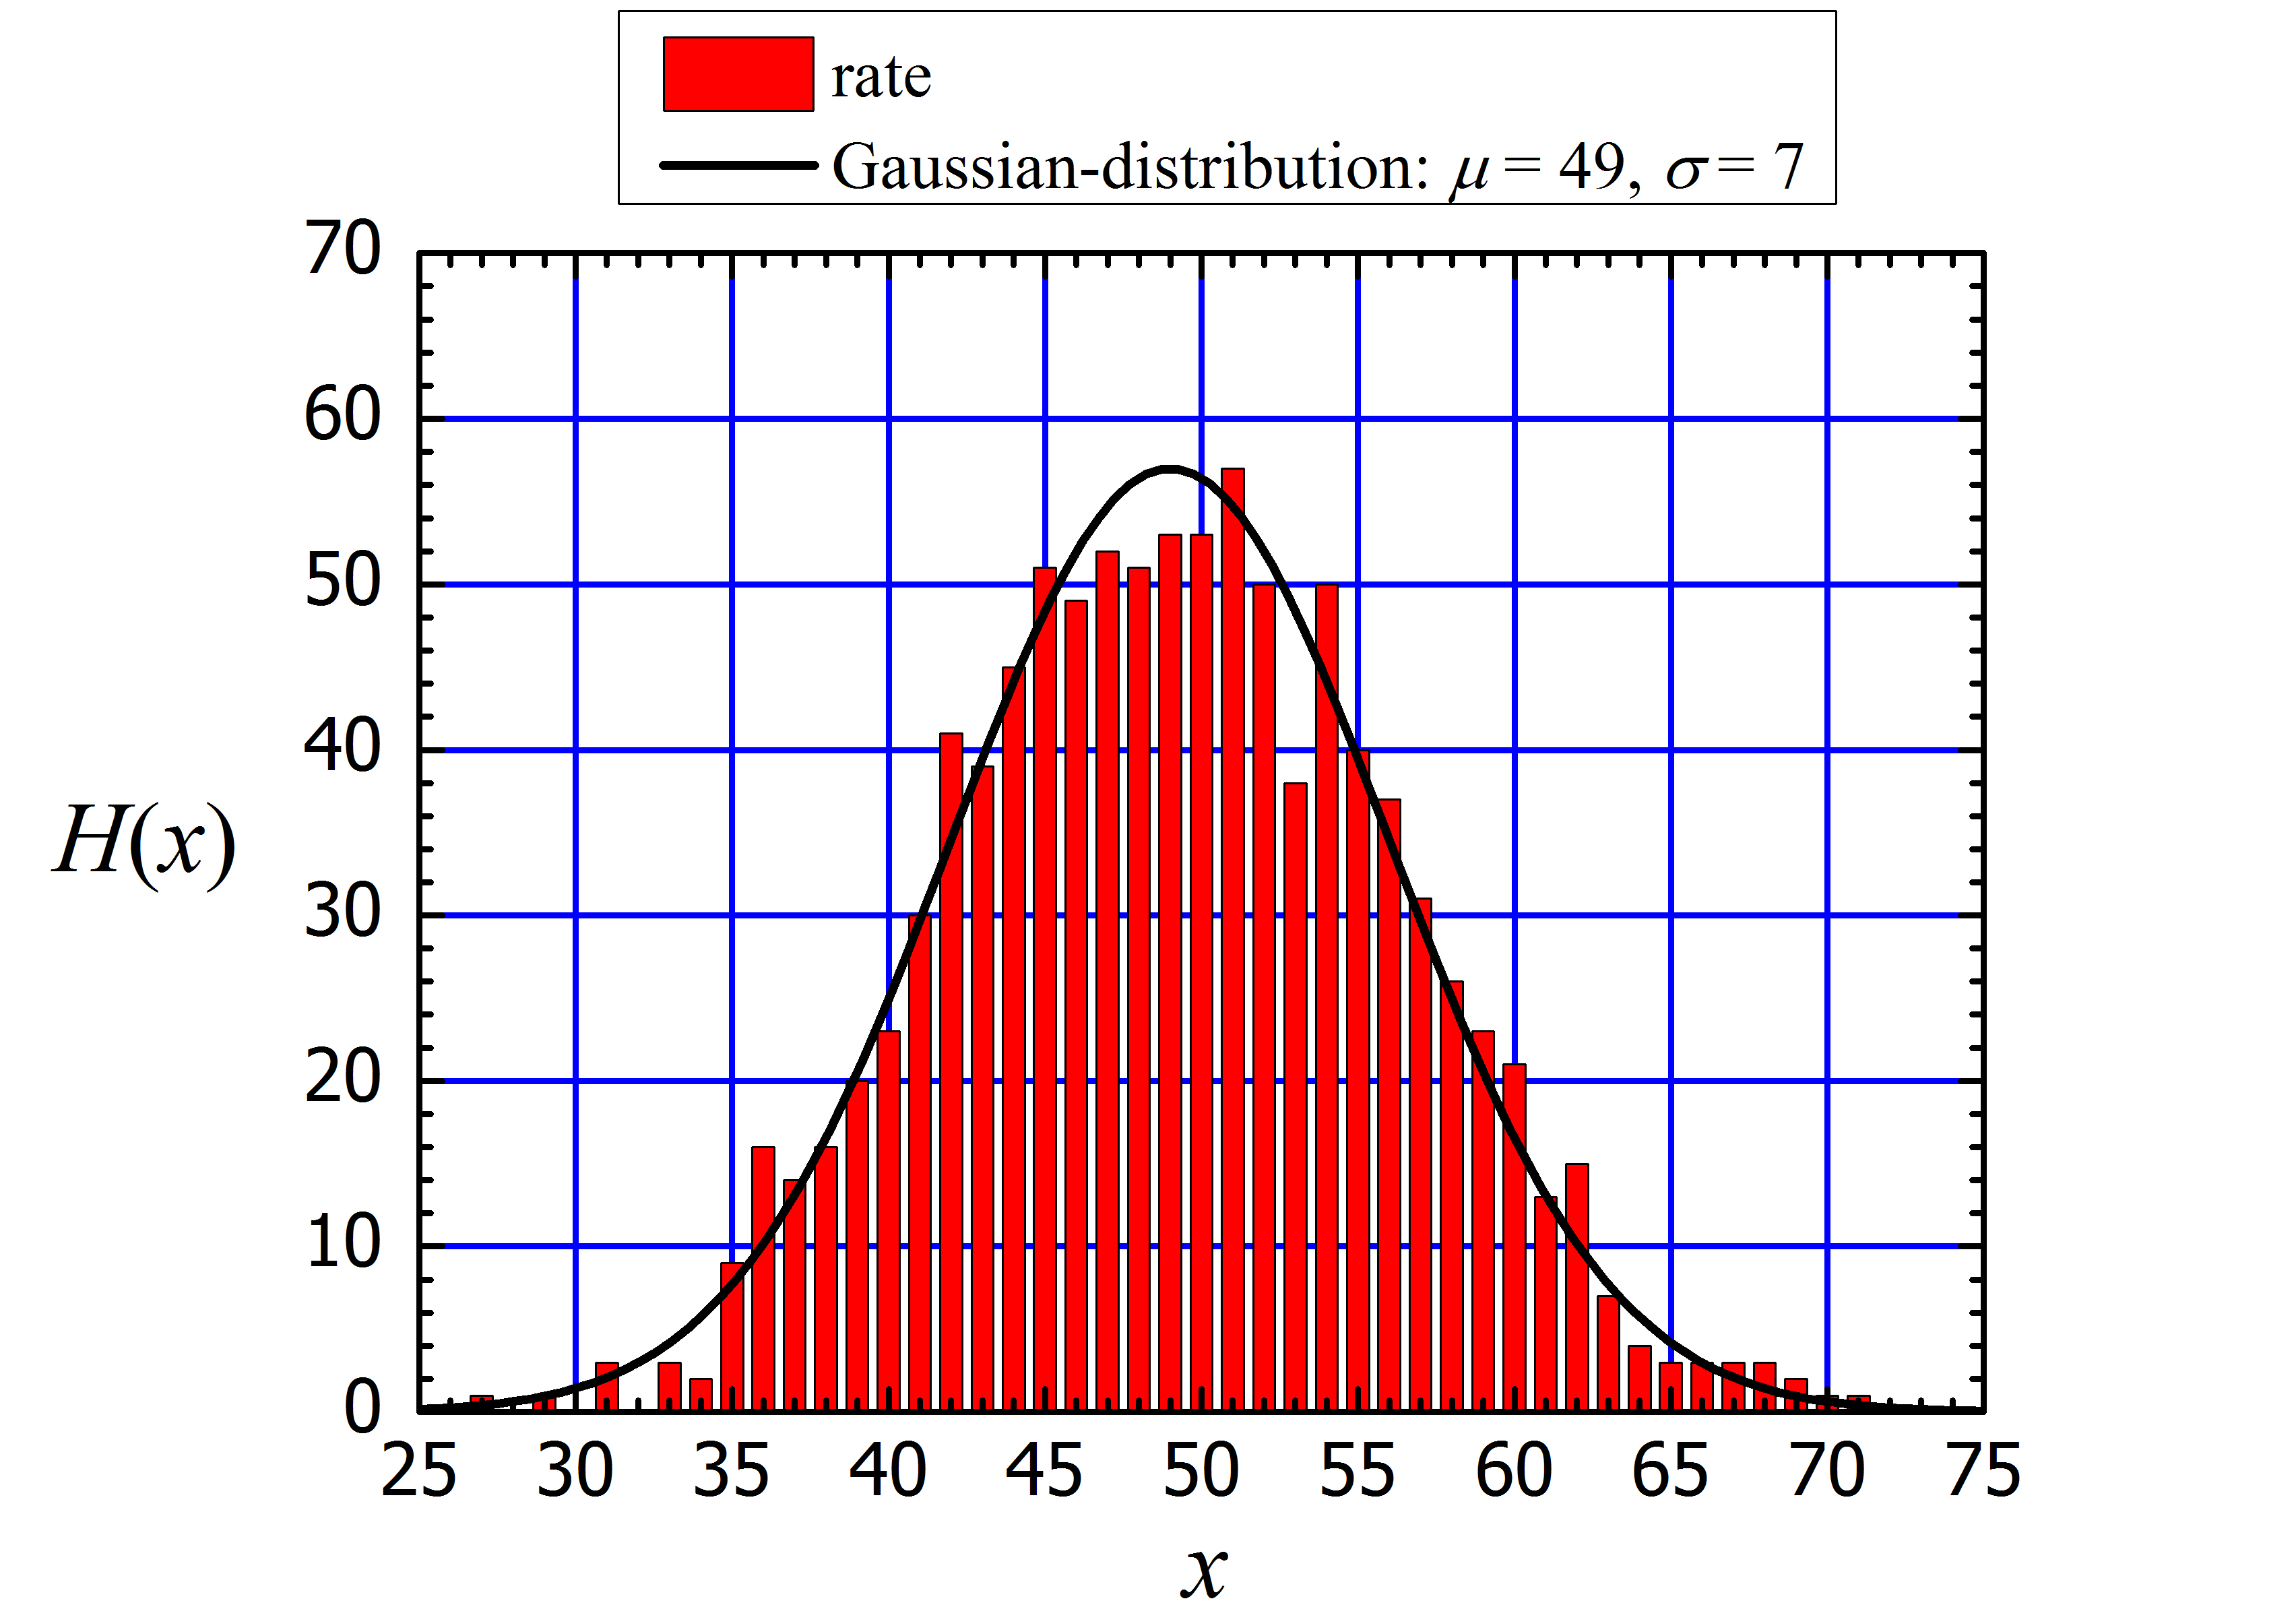
\includegraphics[width=0.7 \textwidth]{Poisson-Messung-mu-49.jpg}
\caption{Absolute rates for 1000 random samples from a \eigen{Poisson}-distribution with set expectation value $\mu=49$ in comparison to the density function $1000 \cdot f(x)$ for the \eigen{Gaussian}-distribution} \label{abb_pois_n_1000}
\end{center}
\end{figure}~\\[0,3cm]

%Verd�chtig sind Messreihen, bei denen die empirischen deutlich kleiner als die theoretischen Standardabweichungen sind. Hier liegt meistens eine Korrelation innerhalb der Impulsfolge vor. Bei Z�hlmessungen treten diese Effekte insbesondere bei hohen Z�hlraten auf, die entweder vom eigentlichen Detektor oder der Nachfolgeelektronik nicht mehr richtig aufgel�st werden. (Es liegt somit ein Totzeitproblem vor.) Sehr breite empirische Verteilungen deuten wiederum auf �u�ere St�reinfl�sse hin. Hier liefern St�rimpulse, die weder der Messgr��e noch dem Untergrund zugeordnet werden k�nnen, zus�tzliche Beitr�ge zum gemessenen Effekt. \\[0,3cm]

Fig.\ref{abb_abs_hfkt_gauss} shows the same measurement values again plotted with random measurement deviations $\pm~2\sigma_\mathrm B = \pm~2 \cdot \sqrt{H(x)}$ of the absolute rate function $H(X=x)$. This plot could be the result of a evaluation of an experiment. Please note that the empirical expectation value is used for the \eigen{Gaussian}-function and the density function was multiplied with the value 1000. The empirical values agree very well with the \eigen{Gaussian} approach. This approximation is quite reasonable. 
   
\begin{figure}[htbp]
\begin{center}
\subfigure[Absolute rates in comparison to the density function $1000 \cdot f(x)$ for a \eigen{Gaussian}-distribution $(\mu=49.2)$ \label{abb_abs_hfkt_gauss}] {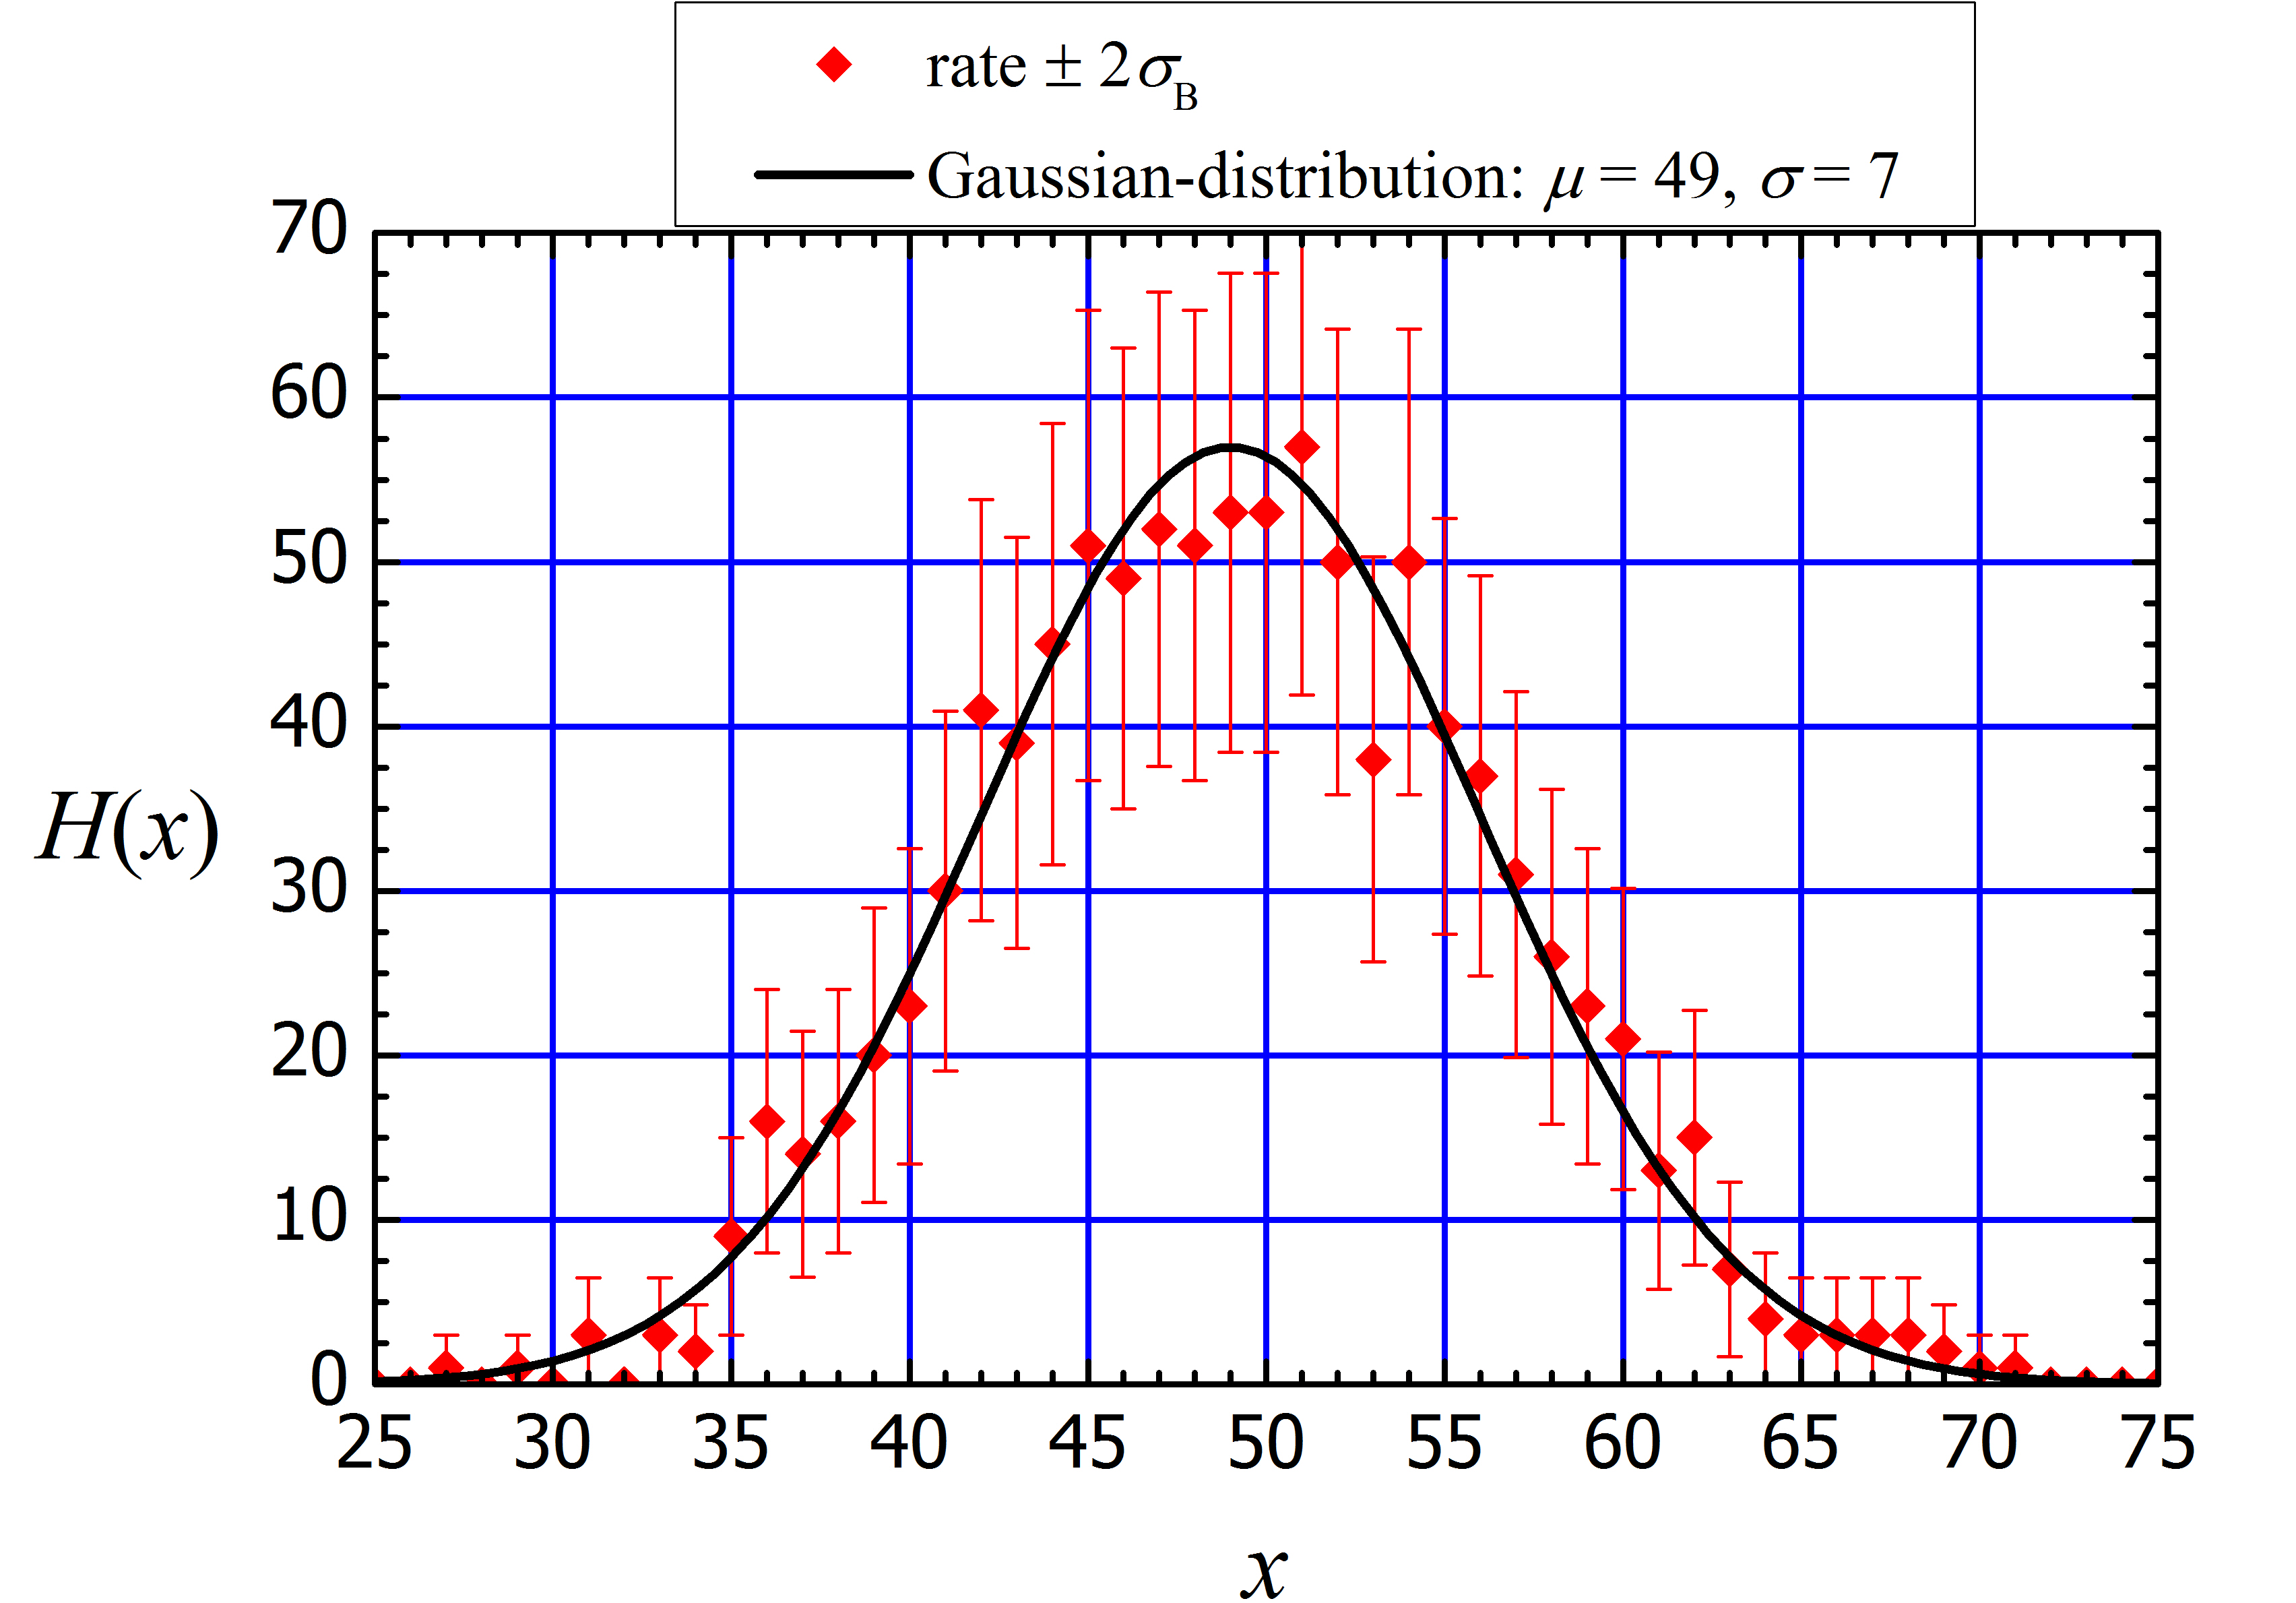
\includegraphics[width=0.7\textwidth]{Poisson-Messung-mu-49-vs-gauss.jpg}}
\subfigure[Absolute rates in comparison to the values of a theoretical \eigen{Poisson}-distribution $(\mu = 49.2)$ \label{abb_abs_hfkt_pois}] {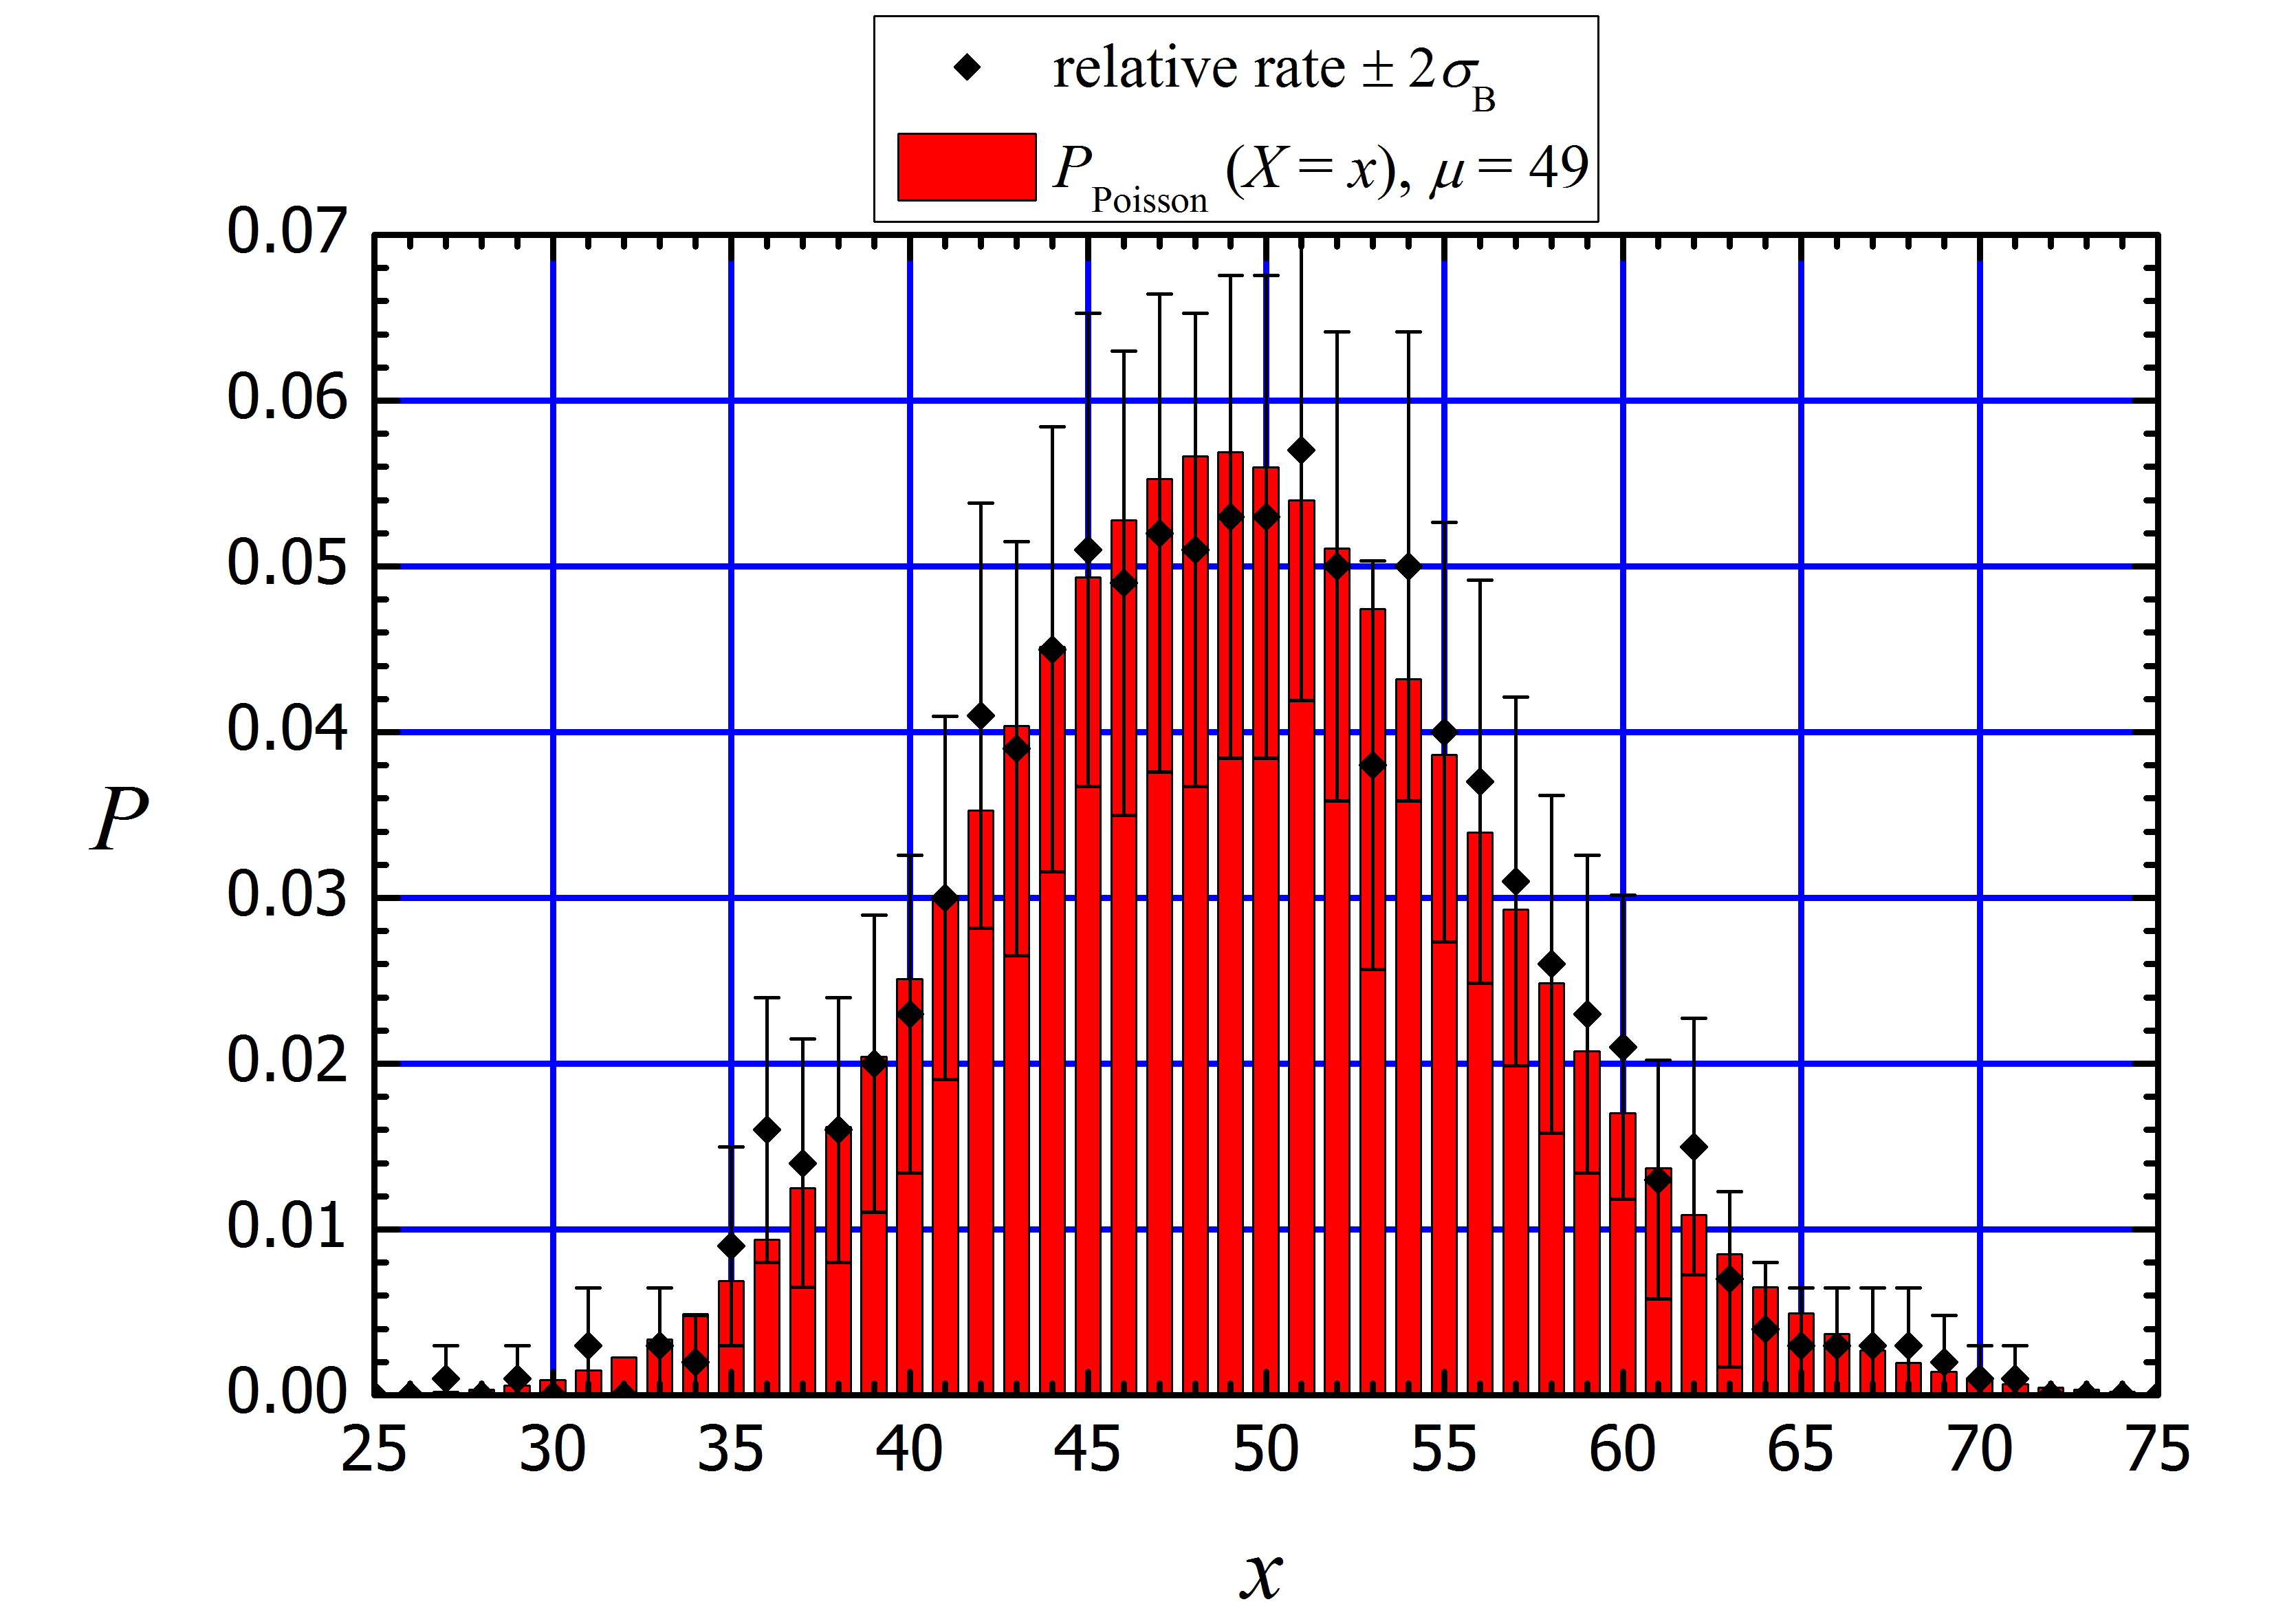
\includegraphics[width=0.7\textwidth]{Poisson-Messung-mu-49-vs-poisson.jpg}}
\caption{1000 random samples from a \eigen{Poisson}-distribution with a set expectation value $\mu=49$ including a random measurement fluctuations ($\pm~2\sigma_\mathrm B$-uncertainty)}\label{abb_messung_pois_vs_gauss}
\end{center}
\end{figure} ~\\[0,3cm]

An illustration like in Fig. \ref{abb_abs_hfkt_pois} is easier to create. Here only the probability function of the \eigen{Poisson}-distribution for the empirical expectation value, which results from the acquired values, has to be calculated and plotted together with the normalized rates. The result is convincing. For small expectation values (for instance the determination of the background noise in the recent experiment) no possibilities of a test exist, because then the \eigen{Gaussian} approach fails.\\[0,3cm]
Overall the previously mentioned variants of the test are very laborious, especially for big expectation values, if no computing power or corresponding software and/or abilities for using them are available. As an alternative possibility the illustration of measurement data in a probability net is shown in Fig.\ref{abb_wahrscheinlichkeitsnetz}. Here the empirical distribution function (normalized cumulative rates) $S(x)$ is plotted dependent to $\tilde{x}=x+0.5$ (correction of continuity). One has to take care that the values of the cumulative rates are always binomially distributed. Therefore the variance can be calculated according to (\ref{glg_bin_mittelwert}).
In this way calculated double standard deviations are the random measurement deviations for the values of the relative cumulative rate and are therefore important for the position of the error bars in the corresponding plots. 
The x-coordinate of the probability net is distorted in such a way that the \eigen{Gaussian}- distributions result automatically in a line. (Quite often also the limits $\pm~1\sigma_S, ~\pm~2\sigma_S, ~\ldots$ are drawn in.) Through numerical approximation or by sound judgment a line is drawn through a crowd of points of the empirical distribution function at the graphical evaluation.
The y-coordinate of the intersection of a line with the constant at $S(x) = 0.1~\%$ results in the value $x_\mathrm u = \mu_x - 3.09\cdot \sigma$. The y-coordinate of the intersection with the line at the constants $S(x)=99.9~\%$ results in the value $x_\mathrm o = \mu_x + 3.09\cdot \sigma$.

With that and the y-coordinate of the line's intersection with the constant $S(x) = 50~\%$, which equals to the expectation value $\mu_x$, the parameter of the approximated normal distribution can be determined.

\begin{figure}[htbp]
\begin{center}
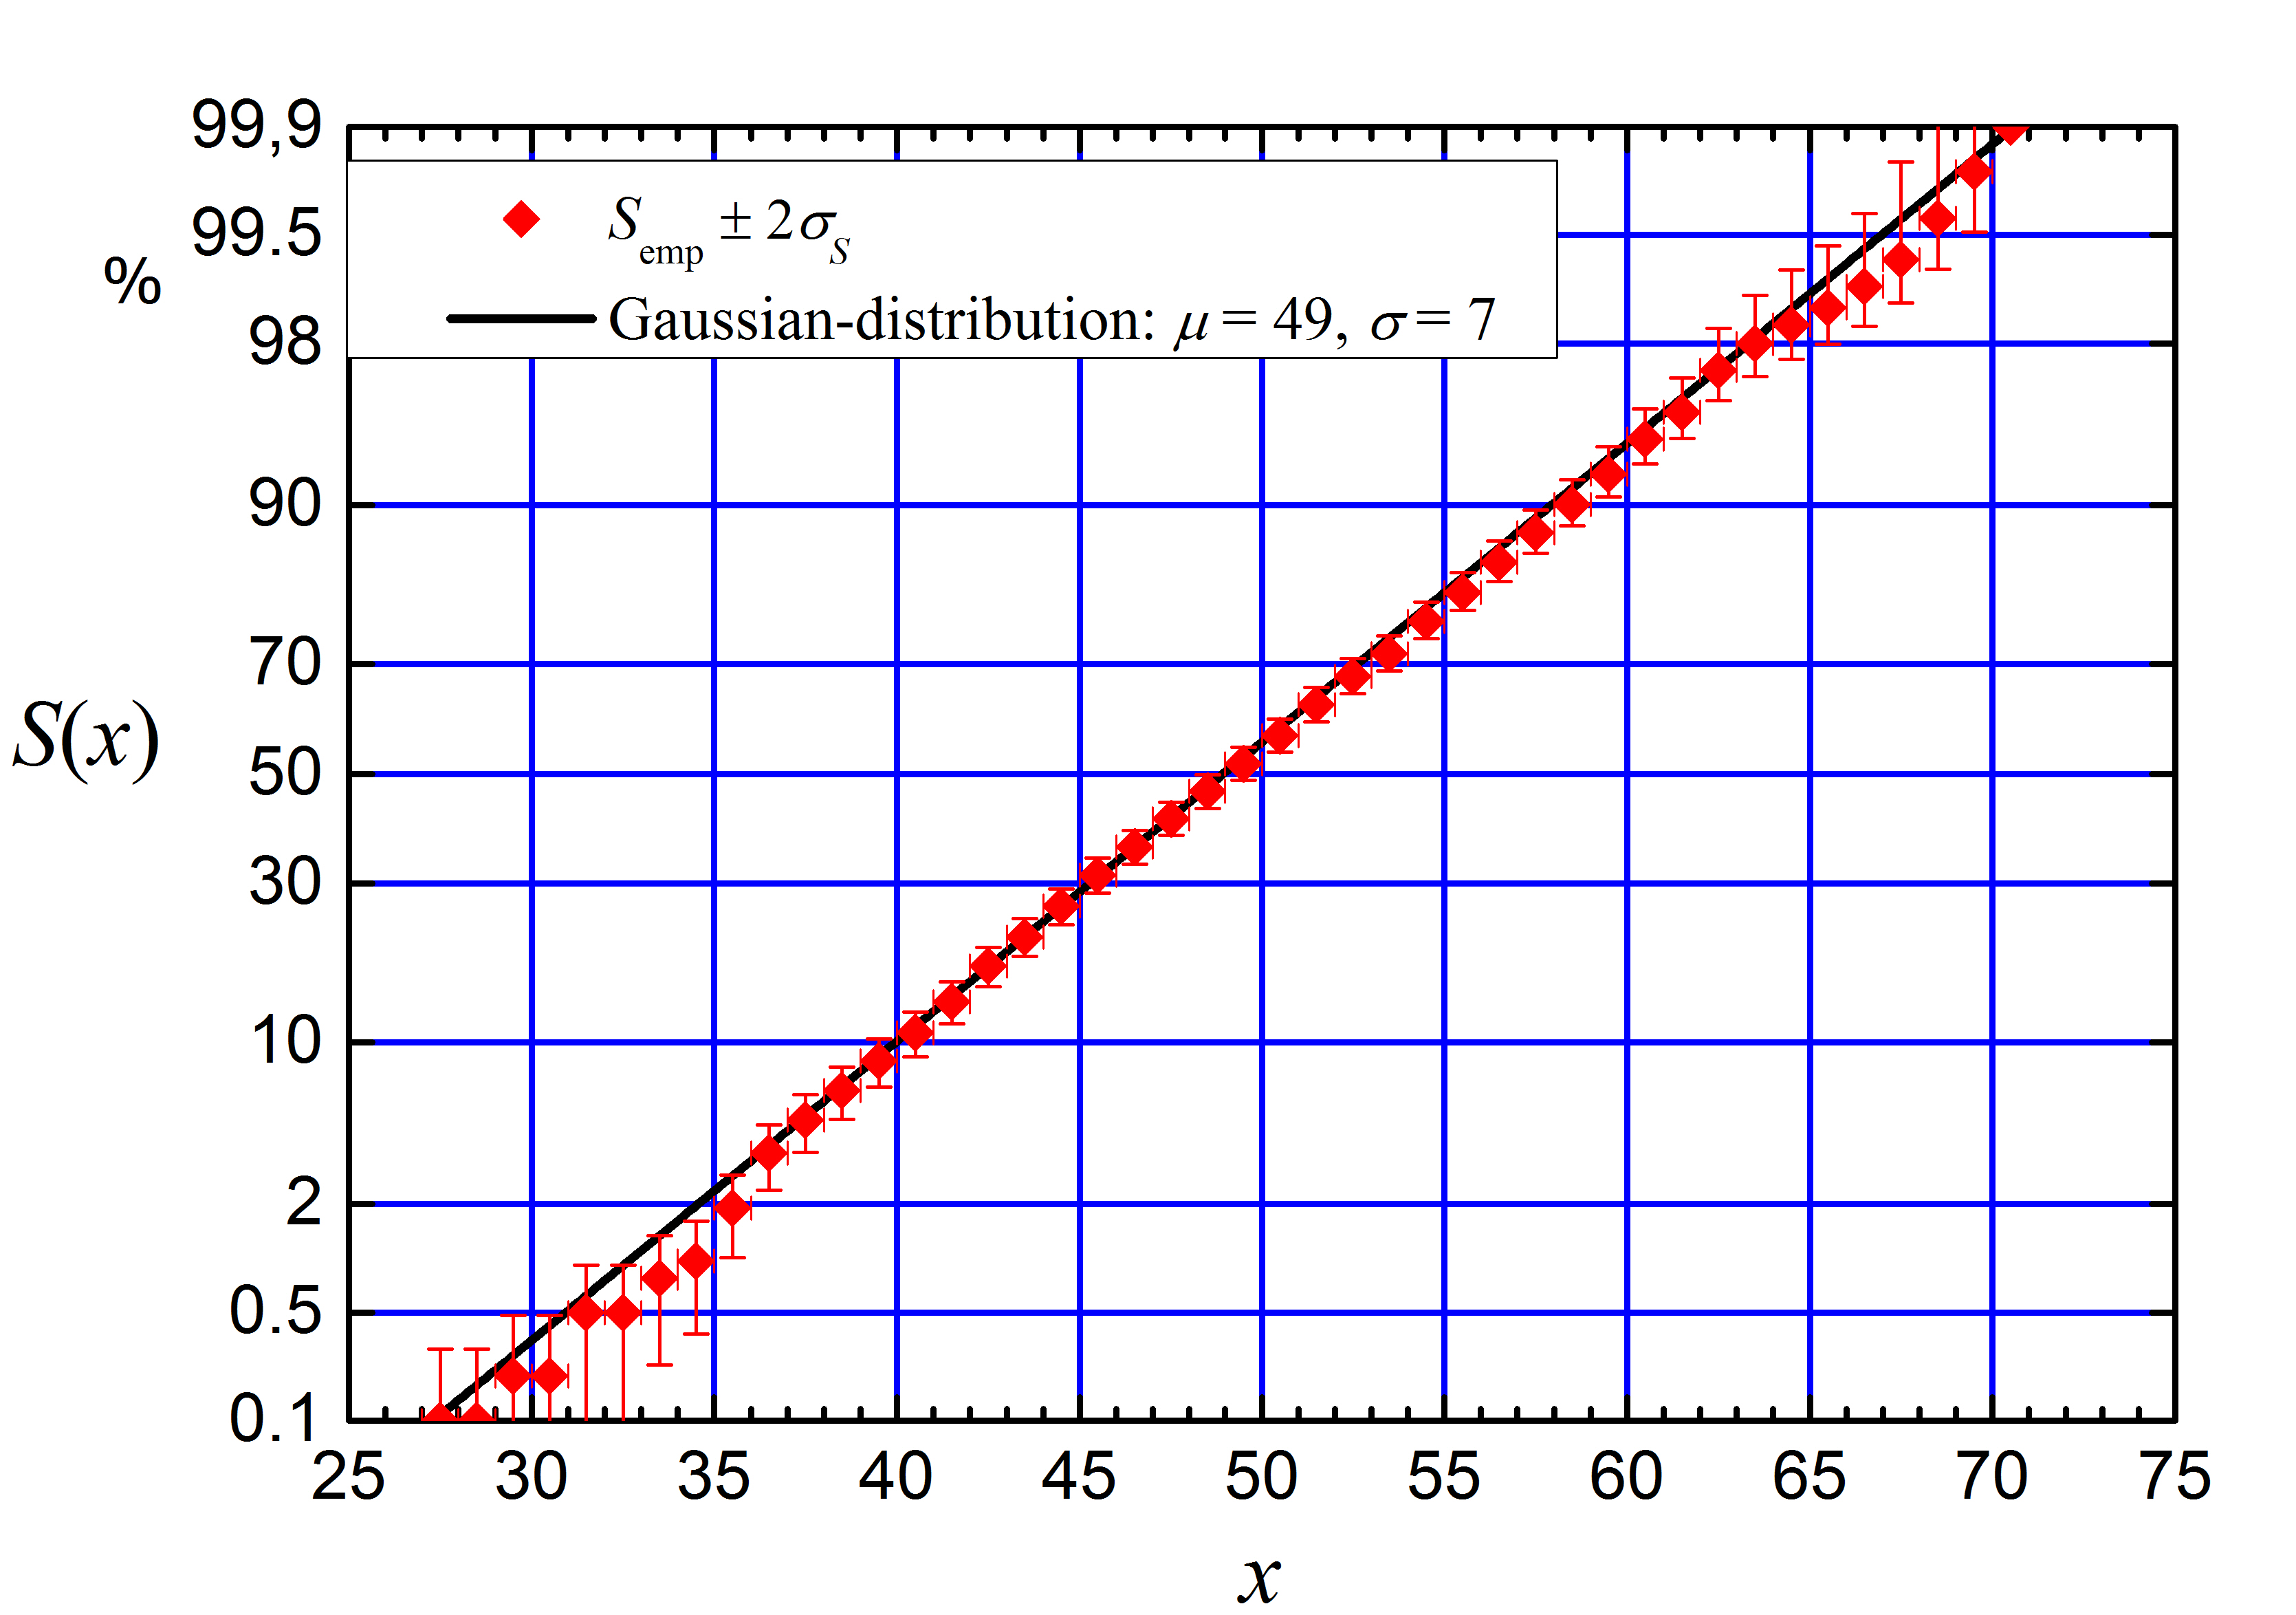
\includegraphics[width=0.7\textwidth]{Poisson-Messung-mu-49-summe.jpg}
\caption{Illustration of the empirical distribution function including random measurement errors ($\pm~2\sigma_S$-Unsicherheit) in the probability net}\label{abb_wahrscheinlichkeitsnetz}
\end{center}
\end{figure}~\\[0,3cm]

Because the normal distribution is a limiting case of the \eigen{Poisson}-distribution, the \eigen{Gaussian}\textit{propagation of uncertainty} is valid for calculating the random measurement errors. It shall be demonstrated with the following simple example. \\ [0,3cm]
The net counting rate $Z_\mathrm n = Z_\mathrm b - Z_0$ represents the difference of the gross counting rate $Z_\mathrm b = \nicefrac{N_\mathrm b}{t_\mathrm b}$ and the background/zero counting rate $Z_0 = \nicefrac{N_0}{t_0}$. The gross effect of $N_\mathrm b$ impulses is evaluated in the gross acquisition time $t_\mathrm b$ and the zero effect $N_0$ is evaluated within the acquisition time of zero effect $t_0$. The standard deviation of $N_\mathrm b$ and $N_0$ are $\sqrt{N_\mathrm b}$ resp. $\sqrt{N_0}$, because they are counting measurements. According to the \eigen{Gaussian} propagation of uncertainty the statistics of the net counting rate can be expressed as:

\begin{eqnarray}
\sigma_\mathrm n^2 ~~=~~ \frac{N_\mathrm b}{t_\mathrm b^2} + \frac{N_0}{t_0^2} ~~~\rightarrow ~~~ \sigma_\mathrm n &=& \frac{1}{t_\mathrm b} \cdot \sqrt{N_\mathrm b + \frac{t_\mathrm  b^2}{t_0^2}\cdot N_0} \label{glg_sigma_netto_0}
\end{eqnarray}
At equal acquisition times $t_\mathrm b = t_0 \equiv t_\mathrm{mess}$ the expression can be simplified to:
\begin{eqnarray}
\sigma_\mathrm n &=&  \frac{\sqrt{N_\mathrm b + N_0}}{t_\mathrm{mess}} \label{glg_sigma_netto_1} 
\end{eqnarray}
Random measurement errors of the time are neglected in those important discussions, because the are much smaller im comparison to the statistical "`counting errors"'. 


\subsection{The \eigen{Geiger-M�ller-}counter (GMC)}\label{kap_gmz}

The ionizing radiation sent out by radioactive isotopes can be measured by diffierent \linebreak 
radiation detectors. For instance gas ionization detectors, excitation detectors and semi-conductor detectors can be used.\\[0,3 cm]
The GMC belongs to the gas ionization detectors. Here the created charge carriers (electrons and ions)
travel to the electrodes due to an electric field inside the detector and release with gathered charge quantity a registrable impulse in the measurement device.

As shown in Fig.\ref{abb_impulszahl-spannung} the applied detector potential strongly influences the created charge quantity and therefore the height of the impulses or the current is dependent on the circuit of the measurement device.
 
\begin{figure}[htbp]
\begin{center}
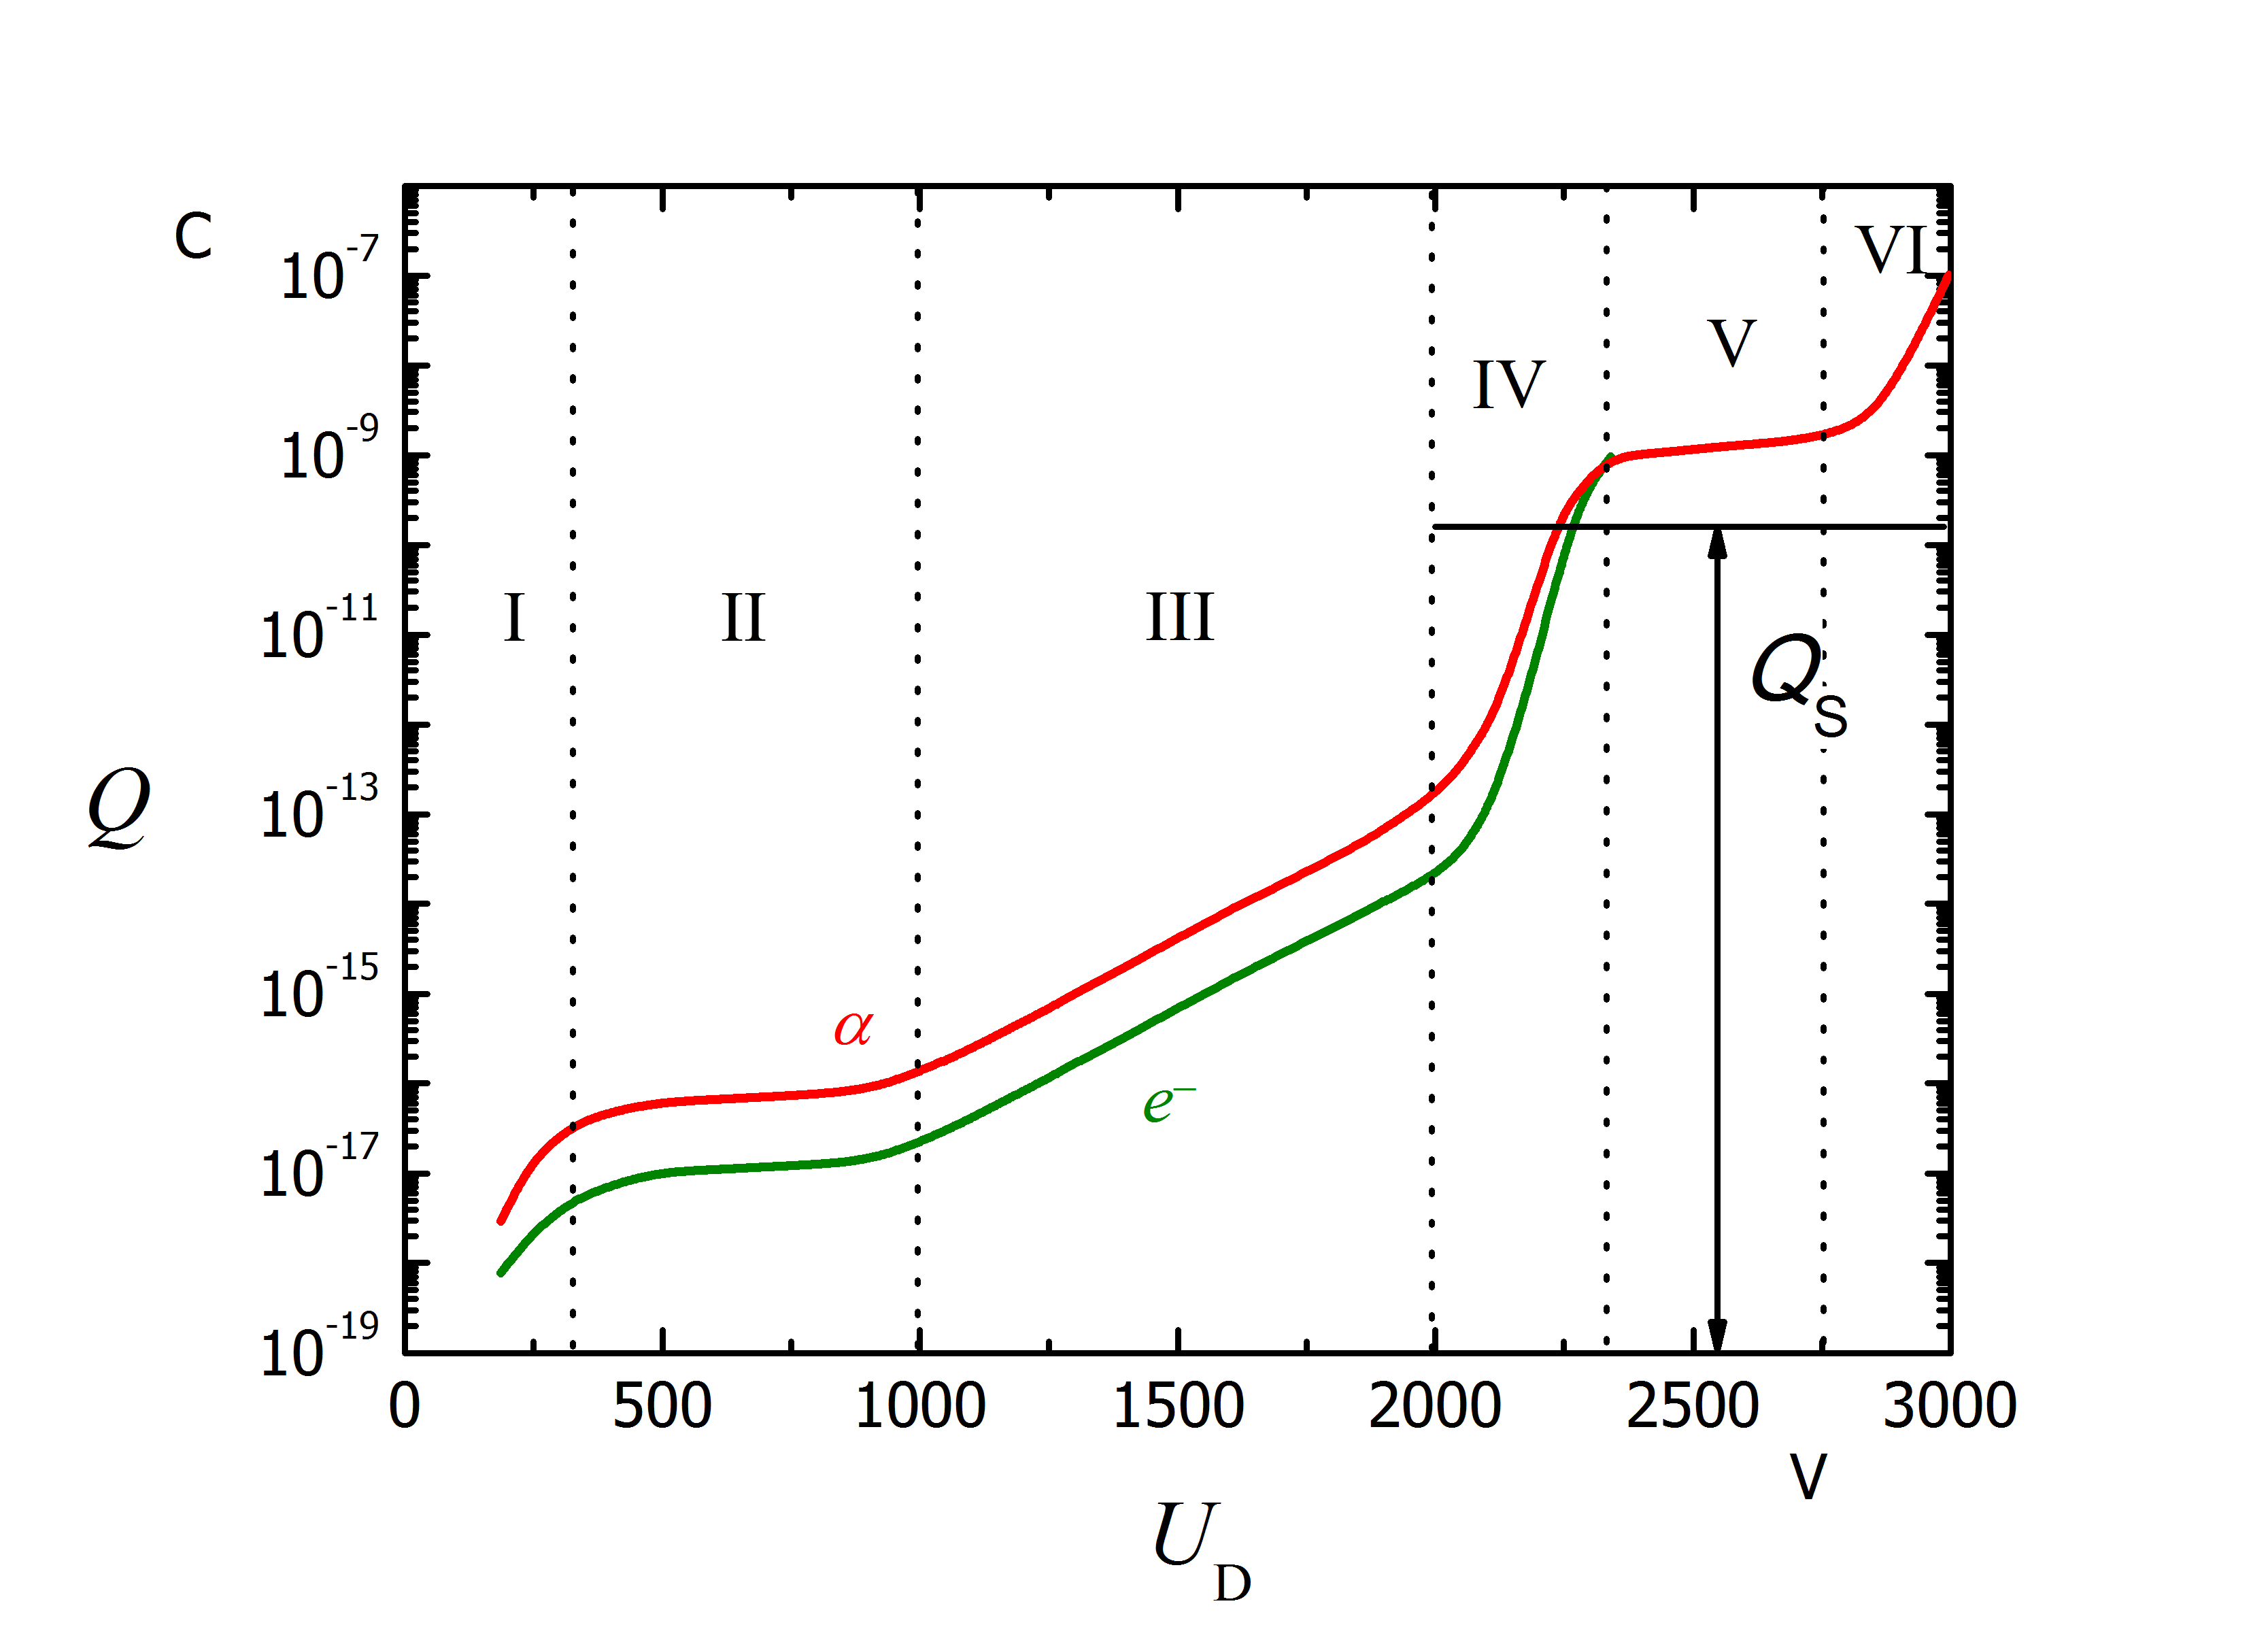
\includegraphics[width=0.7\textwidth]{Gasionisationsdetektoren.png}
\caption{The acquired charge quantity $Q$ as a function of the detector potential $D_\mathrm U$ at a gas ionization detector (schematic illustration)}\label{abb_impulszahl-spannung}%
\end{center}
\end{figure}~\\
The different ranges characterize the operation principle of the different gas ionization detectors.
The range of the curve can be categorized as one of the following::
\begin{description}
	\item[I] -- \textit{The range of recombination}: The primarily created charge carriers recombine on their way to the electrodes due to the too low detector potential/ field strength. No measurements can be performed.
	\item[II] -- \textit{The range of saturation:} All charge carriers created by primary ionization are gathered at the electrodes. Through that it is possible to conclude the particle species resp. their energy by the charge quantity resp. the height of the impulse with an ionization chamber operating in this range
	\item[III] -- \textit{The proportional range:} The occurring impact ionization by accelerated electrons from the primary ionization cause a secondary ionization, which is in this range proportional to the primary ionization. From that one can - similarly to the ionization chambers - deduce the species and energy of the particles in a counter tube operating in this range. The signal is amplified by a factor up to 3 already in the counter tube due to impact ionization.
	\item[IV] -- \textit{The range of limited proportionality:} Secondary ionization predominates the primary effects.
	\item[V] -- \textit{The range of ignition:}	The impact ionization becomes avalanche-like and affects the quantity of created charge independently from the primary ionization. 
	Because of that only counting measurements are possible with a \eigen{Geiger-M�ller}-counter tube operating in this range.
	\item[VI] -- \textit{Continuous discharge:} The high field strength is causing continuous discharge effects, which occur independently from the incidence of ionizing radiation. Glow discharge lamps operating according to this principle.
\end{description}

A radially symmetric field is created in a GMC by a cylindrical cathode and a anode, which is positioned on the axis of the cylinder. Counting gas, in which atoms or molecules get ionized or excited by the interaction with the occurring ionizing radiation, is in that isolated volume. Primary charge carriers created in this way will be multiplied via impact ionization due to the high field strength. Amplifications of a factor from $10^8-$ to $10^{10}-$ are possible. Because of that the primary ionization effect is completely covered. That leads to situation where only counting measurements can be performed with an GMC.
Also due to the big created charge quantity a relatively simple acquisition circuit is realizable. A corresponding circuit diagram is shown in Fig.\ref{abb_gmz}.
\begin{figure}[htbp]
\begin{center}
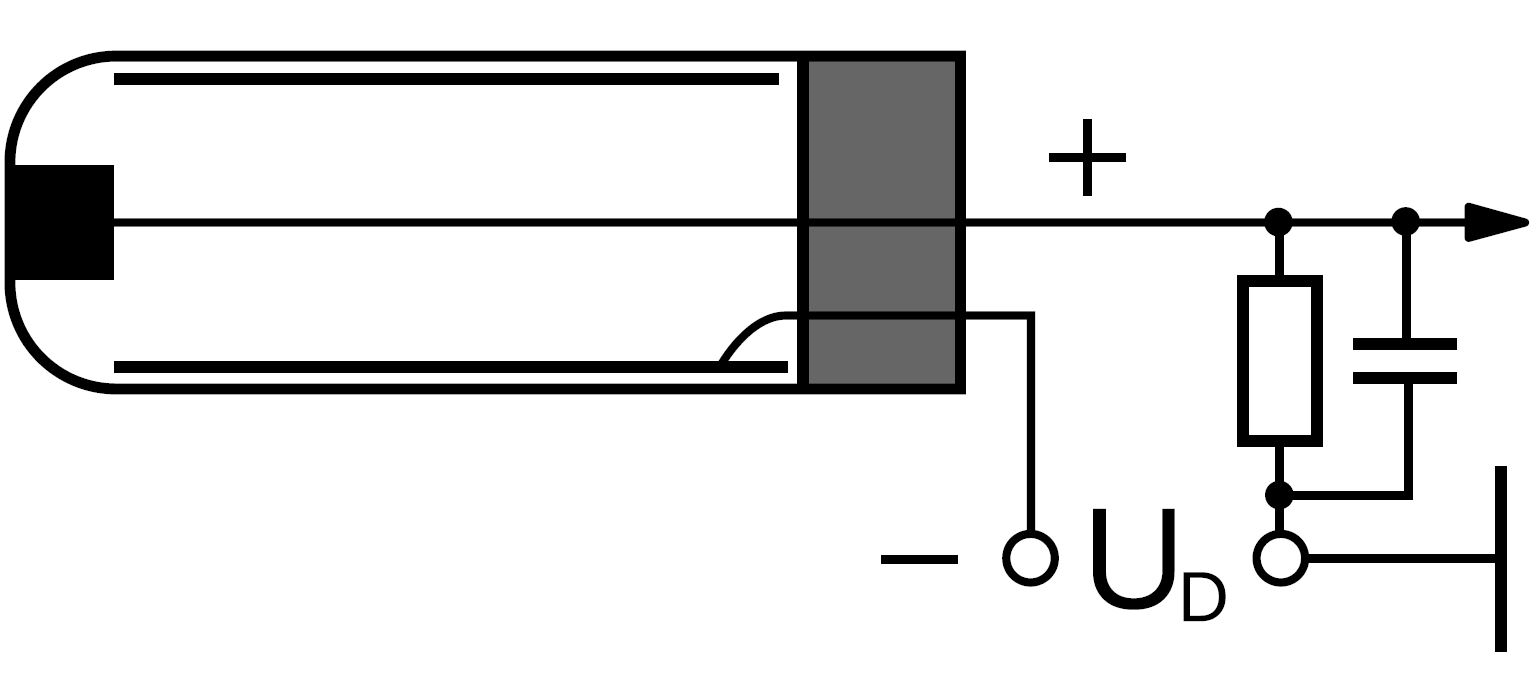
\includegraphics[width=0.4\textwidth]{GMZ}
\caption{Schematic setup and switching principle of a \eigen{Geiger-M�ller}-counter} \label{abb_gmz}
\end{center}
\end{figure}~\\

The ignition range can be reached already at low voltages (some 100~\textsf{V}) depending on the composition and pressure of the counter gas (for instance $\nicefrac{\mathrm{\textsf{Ar}}}{\mathrm{ethanol~vapor}} = \nicefrac{10}{1}$ at 13~\textsf{kPa} total pressure).
The \textit{Counter tube characteristic} can be consulted for determination of the correct working potential of the GMC. For that the counting rate $Z$ has to be plotted dependent to the detector potential $U_\mathrm D$. In this illustration a plateau, where the counting rate is almost independent to the detector potential, should be quite obvious. Deviations of $5~\%$ per 100~\textsf{V} are acceptable here. A steep slope starting at the operation voltage $U_\mathrm E$ can be seen on the left side of the plateau. In the case shown in Fig.\ref{abb_gmz_kennlinie} it starts at the value of $U_\mathrm E = 312$~\textsf{V}. The operation voltage $U_\mathrm A$ is clear on the plateau: approx. 50~\textsf{V} - 100~\textsf{V} above the ignition potential. This corresponds in the present case to a working potential of $U_\mathrm A = 360\ldots 420$~\textsf{V}.
\begin{figure}[htbp]
\begin{center}
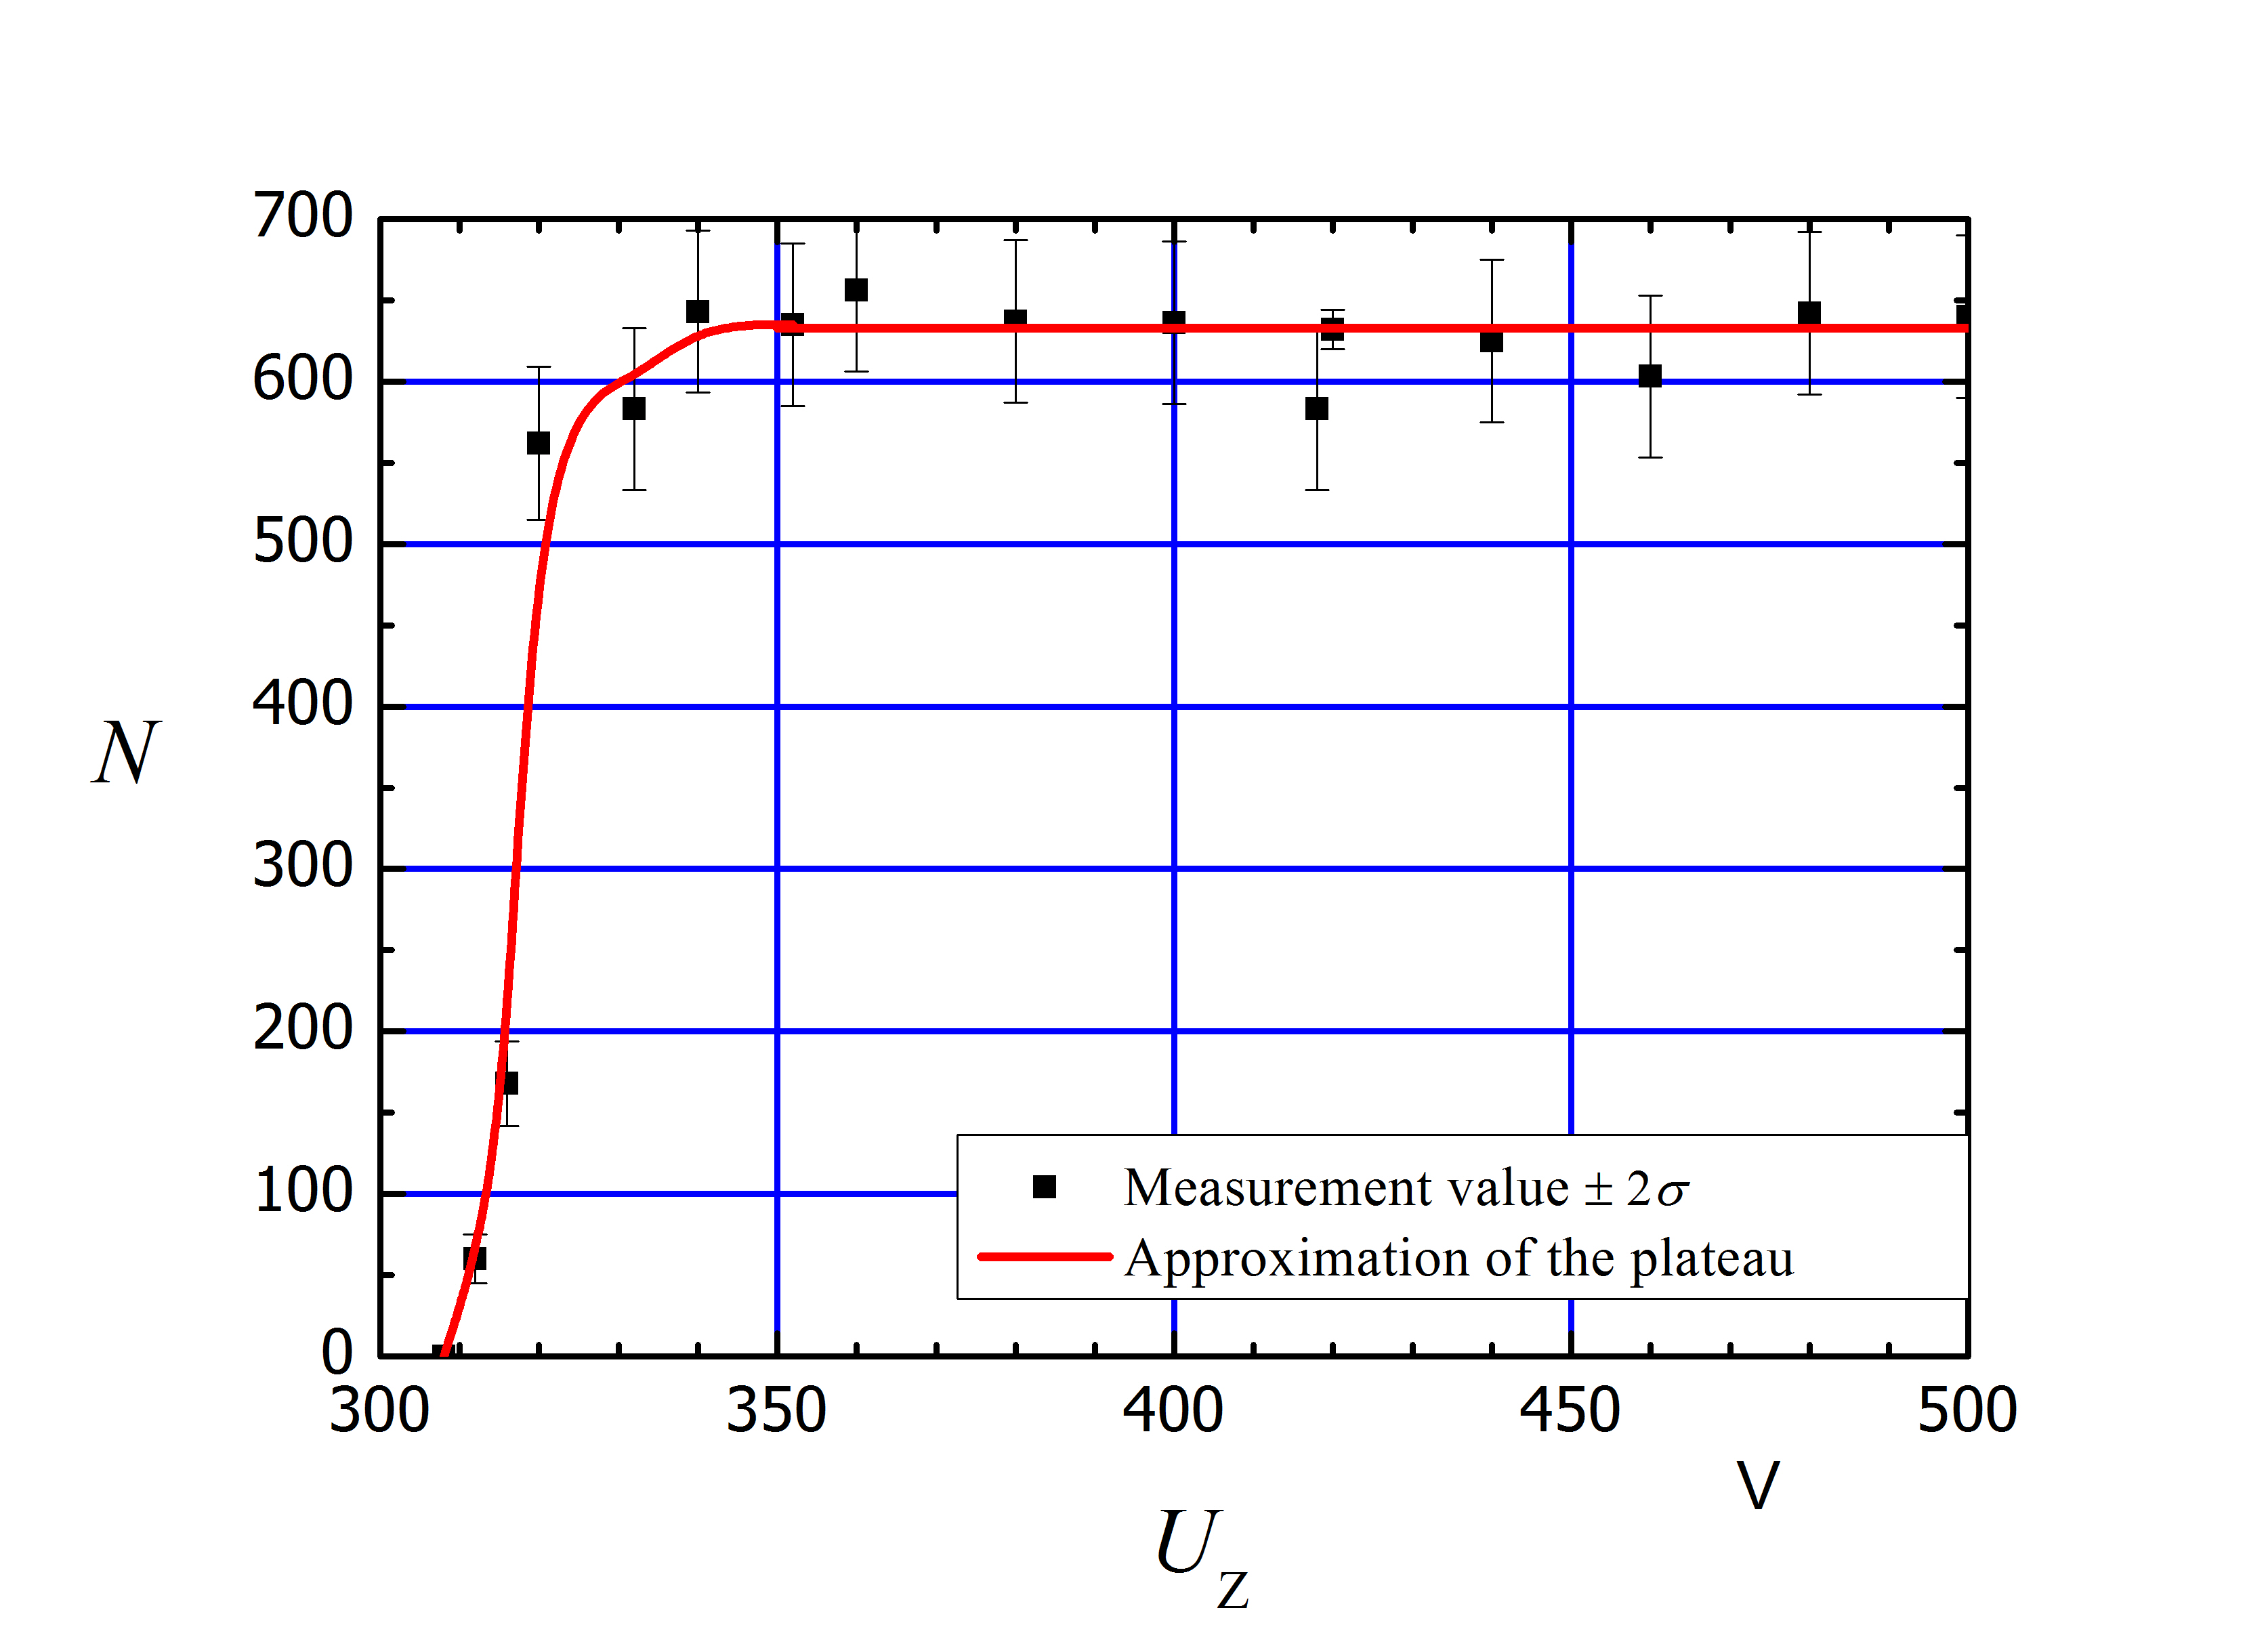
\includegraphics[width=0.7\textwidth]{GMZ-Charakteristik.jpg}
\caption{An example of the characteristic of a counter tube: Determined number of impulses $N$ for a acquisition time period of 120~\textsf{s} as a function of the detector potential $U_\mathrm D$}\label{abb_gmz_kennlinie}
\end{center}
\end{figure}

\section{Experimental execution}

\subsection{Setup}

The samples have to be fixed in the counter tube with the bayonet catch (Fig.\ref{abb_versuchsaufbau}).
Afterwards the PVC-made light protection lid has to be pushed over the measurement head. Then one can start the measurements. ~\\[0,3cm]

The electronics for operating the counter tube, developed in the electronic laboratory of the institute for nuclear and particle physics and shown in Fig.\ref{abb_versuchsaufbau_elektronik}, is connected via USB to a computer. The counter tube voltage is shown on the device at \textit{DET.-VOLTAGE}. The \textit{RATEMETER} shows logarithmically scaled the density of the acquired counting impulses. A virtual Geiger counter is provided for detailed control with LabView by \textit{National Instruments} after opening the program \textit{�Radiometrie \& Zaehlstatistik�}.~\\[0,3cm]
The control of the virtual device shown in Fig.\ref{abb_programmoberflaeche} is quite self-explaining. Both graphs, which are plotted during the measurements and which show the calculated mean value and standard deviation, shall only be used for information. For the experiment necessary values will be copied manually and evaluated.~\\[0,3cm]
\begin{figure}[htb]
\subfigure[Measurement head for the determination of the activity(left to right: Connection cable for the counting device, container for the liquid sample, holder with counter tube and bayonet holder; below the PVC- light protection lid)\label{abb_versuchsaufbau}]
{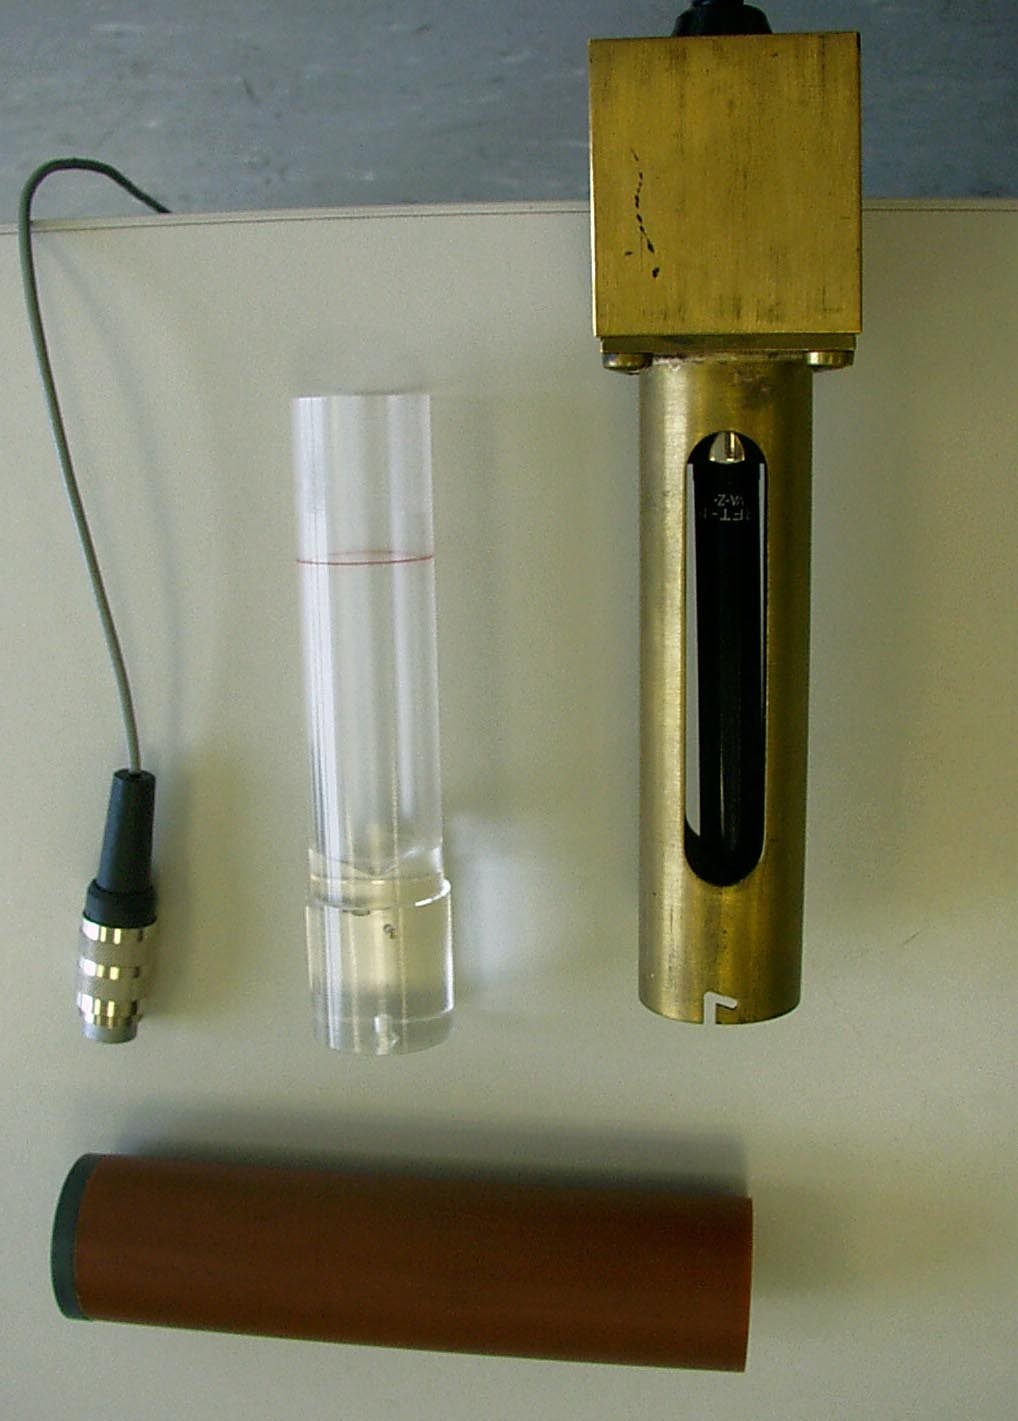
\includegraphics[width=0.5\textwidth]{Versuchsaufbau.jpg}}
\hfill
\subfigure[The counter tube operating device \label{abb_versuchsaufbau_elektronik}]
{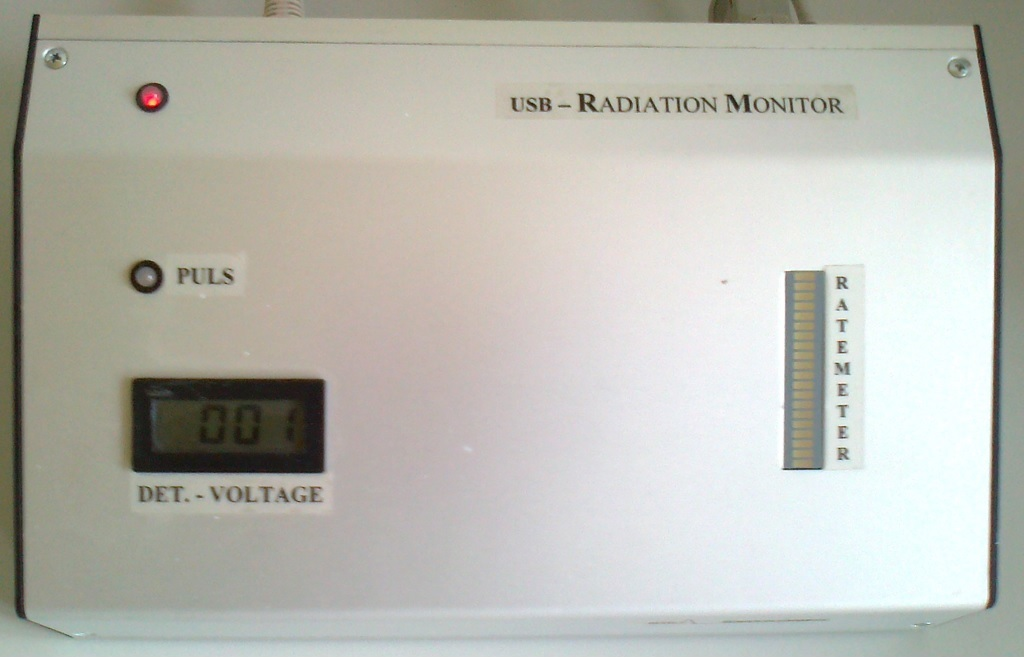
\includegraphics[width=0.48\textwidth]{Versuchsaufbau-Elektronik.jpg}}
\caption{Used devices in the experiment}
\end{figure}~\\
\begin{figure}[htb]
\begin{center}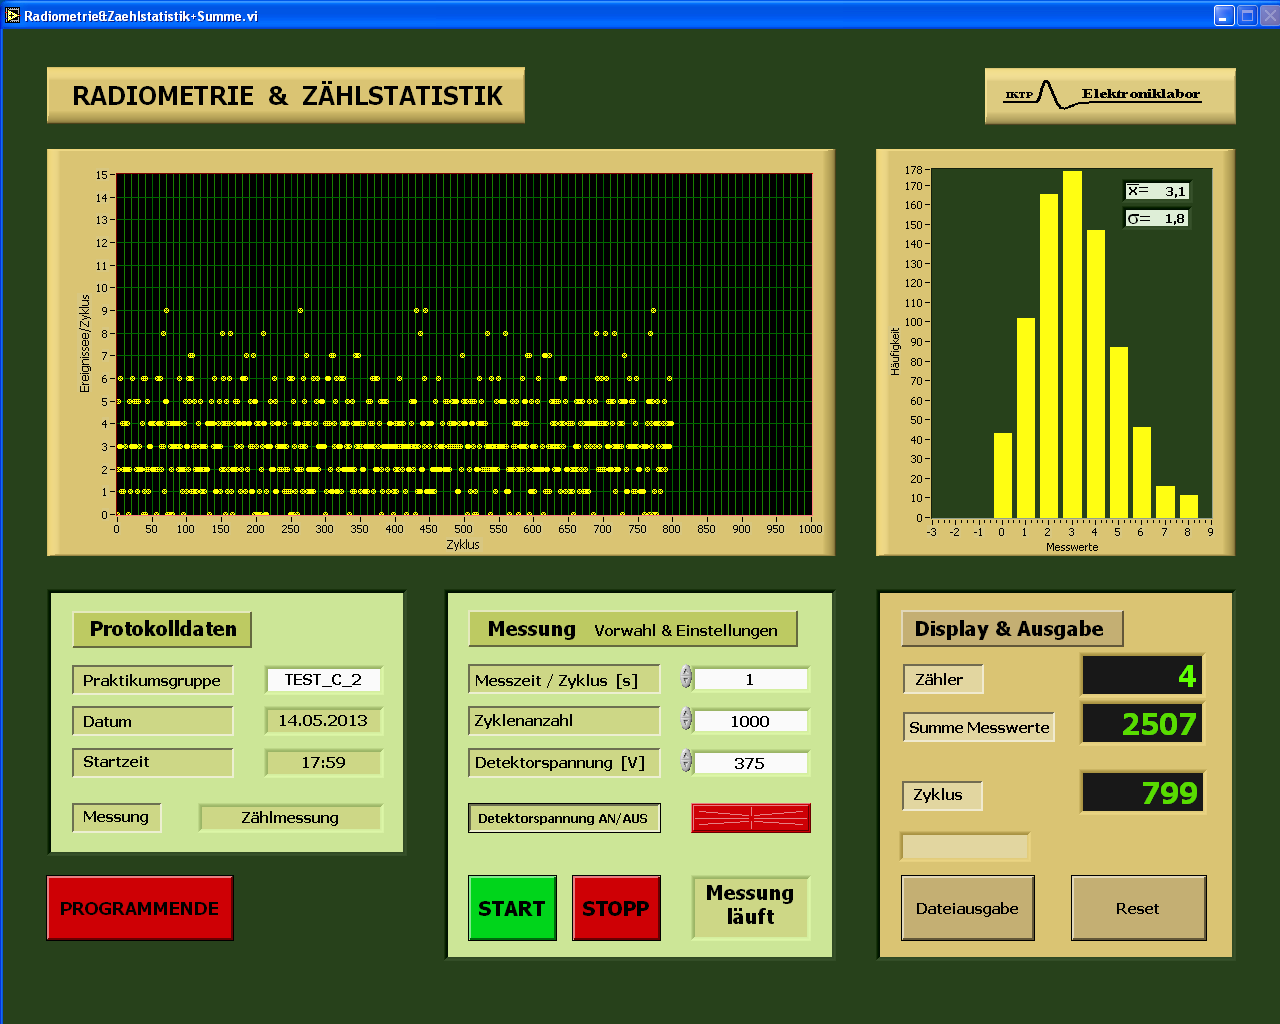
\includegraphics[width=0.8\textwidth]{Programmoberflaeche.png}
\caption{Illustration of the virtual radiation measurement device, developed in the electronic laboratory of the institute of nuclear and particle physics}\label{abb_programmoberflaeche}
\end{center}
\end{figure}~\\
Standard software (\textit{Microsoft Excel}\textsuperscript{\textregistered} and \textit{Microcal Origin}\textsuperscript{\textregistered}) is provided for further evaluations. Using those tools is not necessary for solving the task of the practicum, but it simplifies and accelerates the work significantly. One likes to refer to the available help and device manuals.\\


\subsection{Measurement of the characteristic of the counter tube}

As already mentioned in section \ref{kap_gmz} the working potential $U_\mathrm A$ for the counter tube has to be determined. For this the characteristic of the counter tube has to be acquired. Therefore the working potential $U_\mathrm E$, where the first impulses can be detected, has to be determined beginning at $U_\mathrm D = 290$~\textsf{V}. The counter tube might be defect, if the potential is above 350~\textsf{V}. The measurement values have to be acquired in steps of 2 \textsf{V} in the range of $U_\mathrm E - 6$~\textsf{V}$~~~\leq~~U_\mathrm E~~<~~U_\mathrm E + 6$~\textsf{V}. After that the step sizes can be increased to 20~\textsf{V} - 40~\textsf{V}. The end of the acquired curve is reached at a potential between 460~\textsf{V} - 500~\textsf{V}. \\[0,3cm]
In total 12 - 15 measurement points, which are plotted with their uncertainties for a confidence interval of $\approx 95~\%$ ($\Delta N_\mathrm z = 2\sigma_N = 2 \sqrt{N}$), are sufficient for representing.
The representation of a uncertainty of the potential can be waived, because it is smaller than $\pm~1$~\textsf{V}. The acquisition time has to be chosen in this way that the relative standard deviations $\varepsilon_\sigma$ is $\varepsilon_\sigma \leq 0,05$ for measurement values at the plateau. \\[0,3cm]

The operational potential $U_\mathrm D$, the working potential $U_\mathrm A \approx U_\mathrm E + 50 \ldots 100$~\textsf{V}, the length of the plateau as well as the absolute and relative slope (with the units \textsf{V}\textsuperscript{-1} and $\nicefrac{\%}{100~\mathrm{\textsf{V}}}$) can be determined from the plot $N = f(U_\mathrm D)$.

\subsection{Radiometric determination of potassium}

The radioactivity of potassium compounds allow the determination of concentration by determination of activity. Principally two approaches are feasible for determining the concentration~$c$ from the counting rate~$Z$. \\[0,3cm]
The \textit{absolute procedure} allows, with known efficiency $\eta$ of the measurement setup, the calculation of the activity $A$ and with that the concentration $c$ from the counting rate $Z$. \\[0,3cm]
The \textit{relative procedure} is the more common method. There a calibration curve for the counting rate $Z$ dependent on the concentration $c$ to $Z = f(c)$, which is used for determining the concentration of applying this procedure, is acquired. That approach is useful, when the constants necessary for determining the efficiency, $\eta$, are not sufficiently known or when the constants might vary at changes of concentration during the experiment.
 This possible deviation from the linearity of the relation $Z=f(c)$ is considered by utilizing an experimentally determined calibration curve. \\[0,3cm]
The linear correlation between $Z$ and $c$ is guarantied at the measurement conditions at this experiment. 
One can apply the linear equation:
\begin{eqnarray}
N &=& a\cdot c + b\label{glg_kal_g_koeff} \nonumber
\end{eqnarray}
The coefficient of the slope $a$ and the intersection $b$ will be determined by the values of the counting rate $Z_1$, caused by the known concentration $c_1=4~\nicefrac{\mathrm{\textsf{mol}}}{\mathrm{\textsf{l}}}$, and by the underground counting rate $Z_0$, caused by the concentration of potassium in destilled water $c_0=0$.
The calibration line can be determined via the slope triangle $a = \nicefrac{d_Z}{d_c}$ (see Fig. \ref{abb_kal_gerade}) as:
\begin{eqnarray}
Z &=& \frac{Z_1 - Z_0}{c_1 - c_0}\cdot c + Z_0 \label{glg_kal_gerade_z}
\end{eqnarray}
Because it is $c_0 = 0$ and the same acquisition time $t_\mathrm m$ is available for the counting rates, (\ref{glg_kal_gerade_z}) with the impulse quantity $N$ and with $Z = \nicefrac{N}{t_\mathrm m}$ can be simplified to:
\begin{eqnarray}
N &=& \frac{N_1 - N_0}{c_1}\cdot c + N_0 ~~~~~, \label{glg_kal_gerade_n}
\end{eqnarray}
where $N$, $N_1$ and $N_0$ are the measured impulse quantities for unknown, known and underground concentration.
The unknown concentration $c$ can be determined via:
\begin{eqnarray}
c &=& c_1 \cdot \frac{N - N_0}{N_1 - N_0} ~~~~~. \label{glg_c_bestimmung}
\end{eqnarray}
The calculated concentration $c$ is here considered as a function $c = c(c_1,~N,~N_1,~N_0)$ dependent on four variables. Fig.\ref{abb_kal_gerade} shows a simple illustration of that correlation. \\[0,3cm]
\begin{figure}[htbp]
\begin{center}
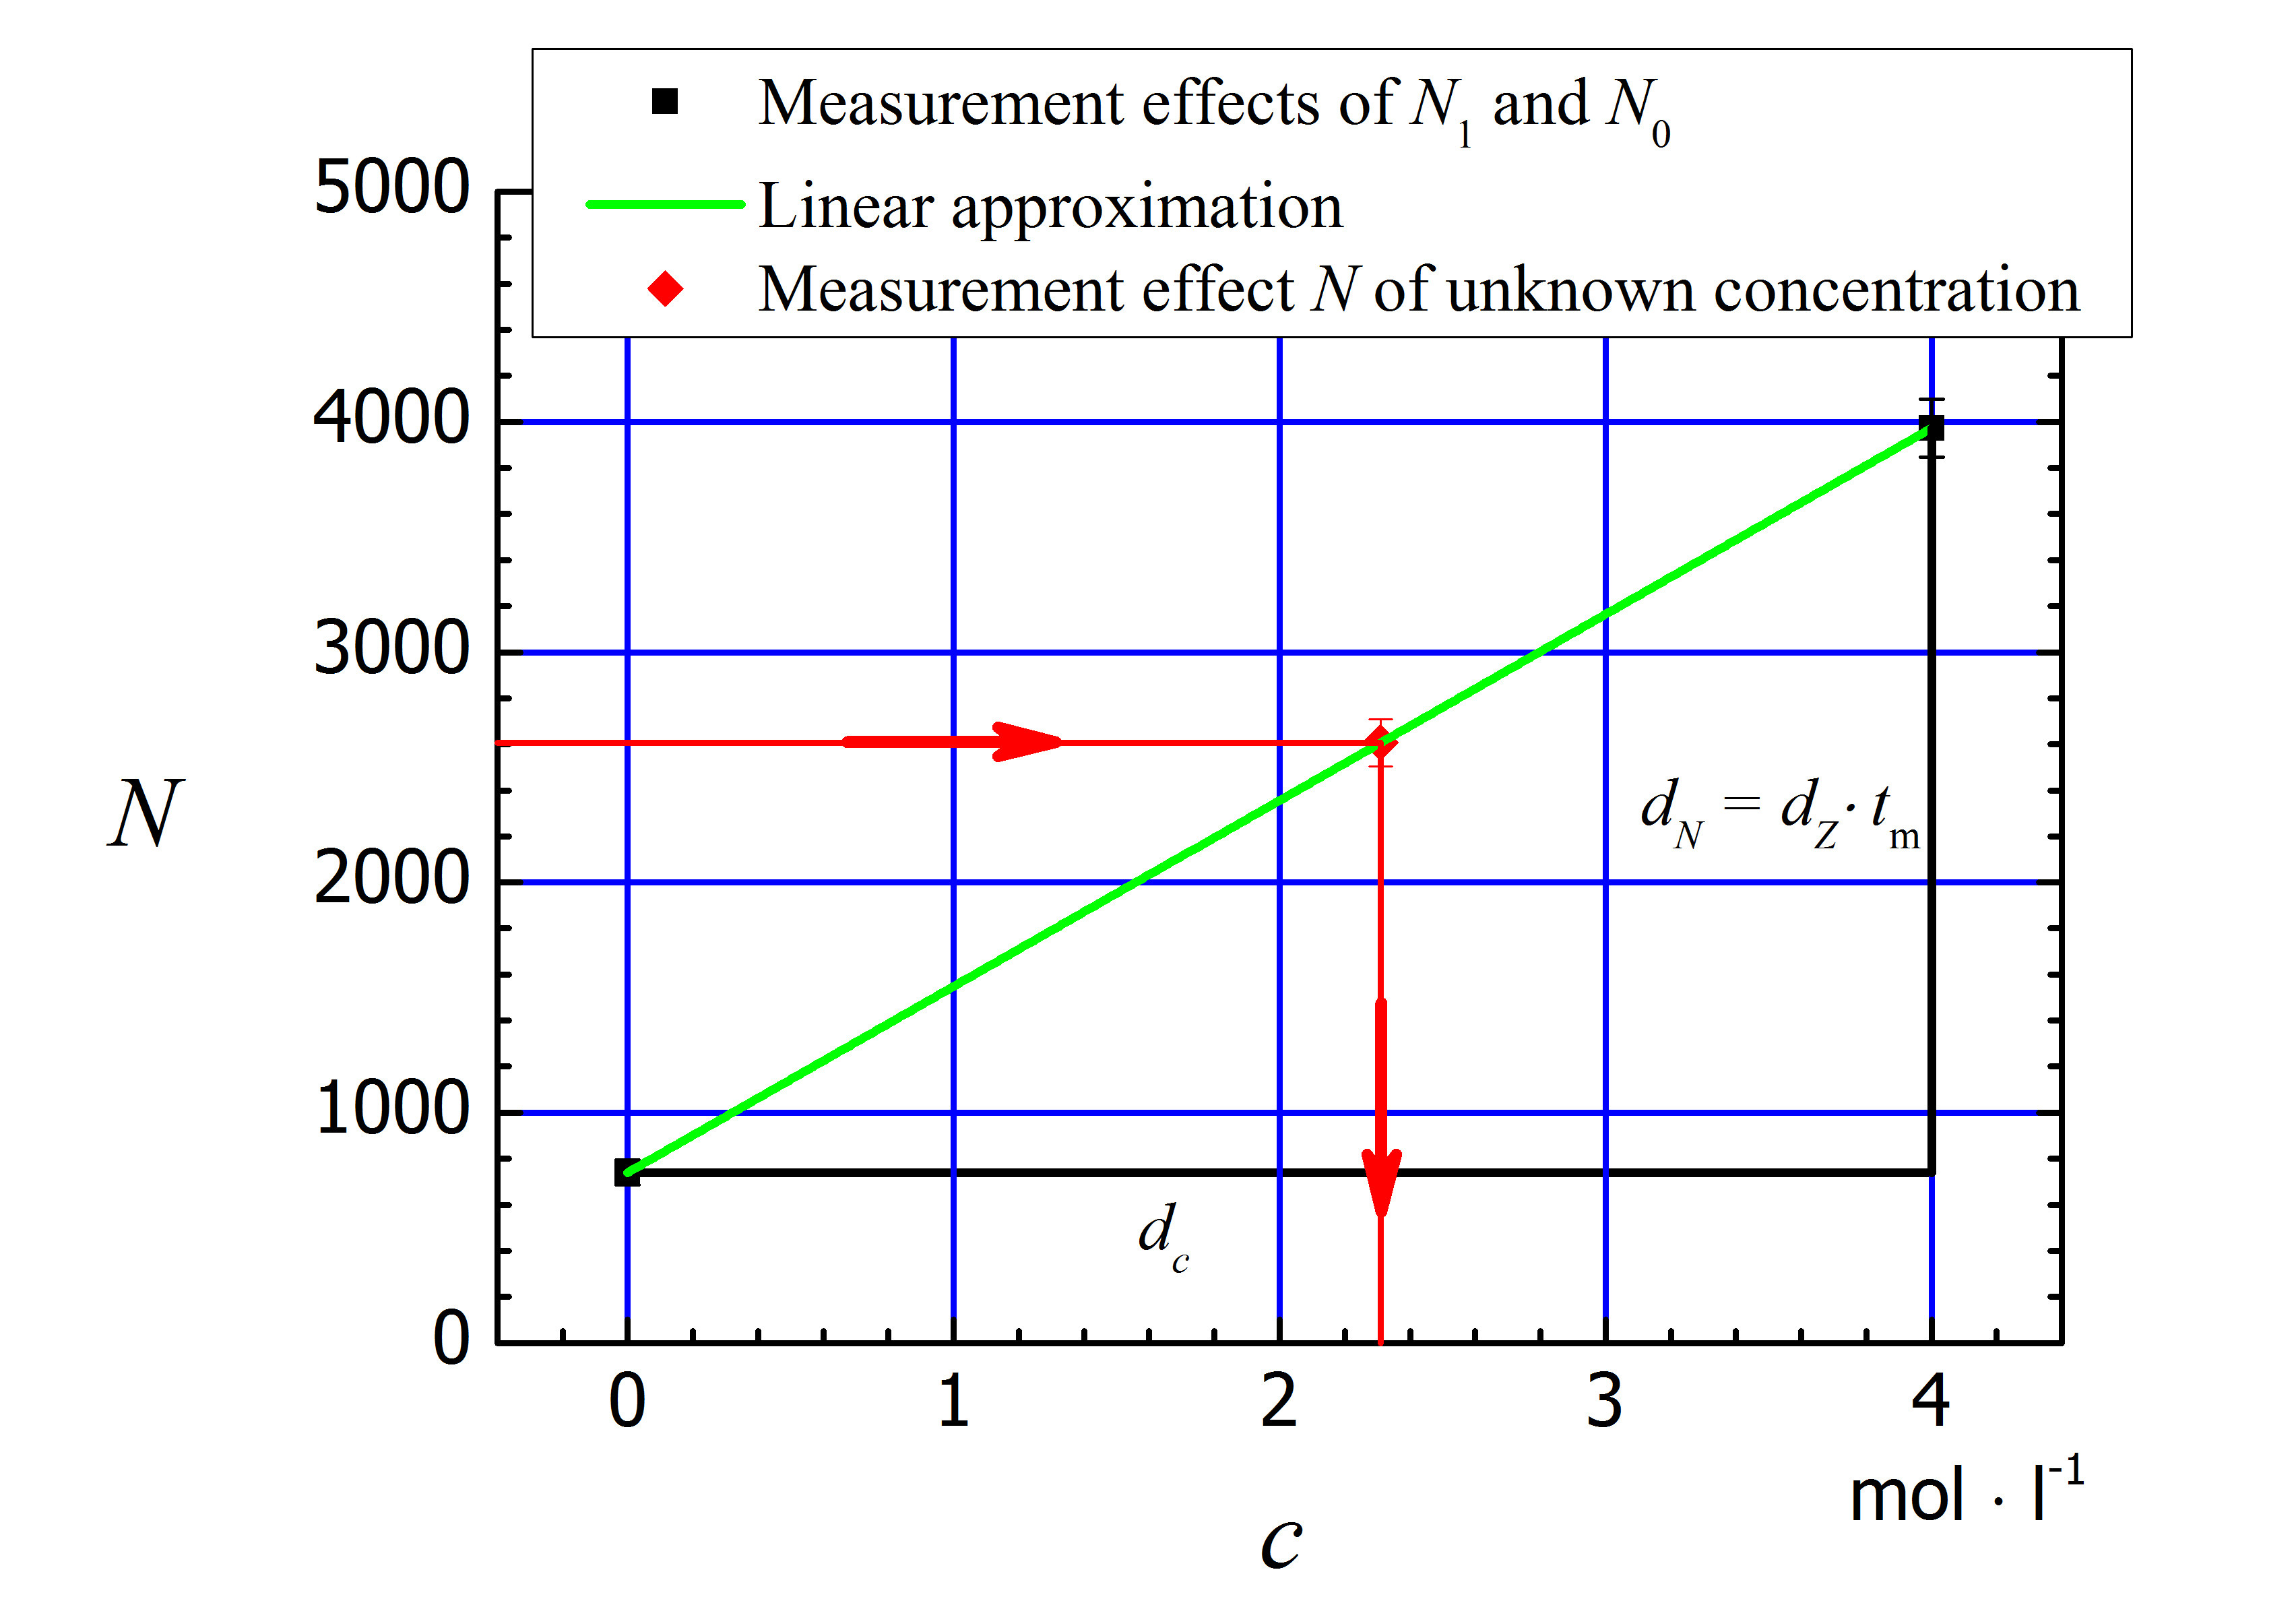
\includegraphics[width=0.7\textwidth]{Kalibriergerade.jpg}
\caption{
Graphical illustration of the measurement effects $N_1$, $N_0$ and $N$ with a $\pm~2\sigma$-uncertainty for an acquisition time of 1000~\textsf{s} for the determination of an unknown concentration (in this experiment $c=2,31~\nicefrac{\mathrm{\textsf{mol}}}{\mathrm{\textsf{l}}}$)  via calibration line, here with slope triangle}\label{abb_kal_gerade}
\end{center}
\end{figure}
An acquisition time of 1000~\textsf{s} is suggested for all three counting measurements.

\subsection{Evaluation of the measurement errors}
All four dimensions for calculating an unknown activity according to (\ref{glg_c_bestimmung}) will be experimentally determined and therefore they are containing errors. Therefore one has to distinguish consequently between \textit{systematic} and \textit{random} errors.
To simplify the formalism it is: 
\begin{eqnarray}
c &=& c_1\cdot f(N,~N_1,~N_0) \nonumber
\end{eqnarray}

The function $f$ is here the quotient 
\begin{eqnarray}
f(N,~N_1,~N_0) &=& \frac{N-N_0}{N_1-N_0}\nonumber
\end{eqnarray}
of the so called net impulse quantity (difference of gross and underground impulse quantities). 
The physical unit of $f$ is 1, because it is a ratio.\\[0,3cm]
The development of the partial derivation to four independent variables $c_1$, $N$, $N_1$ and $N_0$ is necessary for calculating the measurement uncertainty of the concentration $c$.
First it results:
\begin{eqnarray}
\frac{\partial c}{\partial c_1} ~~=~~ f ~~~~~,~~~~~~~~~~~~~~~~~~~~~~~~~~~~ \frac{\partial c}{\partial N_1} &=& c_1\cdot \frac{\partial f}{\partial N_1} ~~~~~, \nonumber  \\
\frac{\partial c}{\partial N} ~~=~~ c_1 \cdot \frac{\partial f}{\partial N} ~~~~~,~~~~~~~~~~~~~~~~~~~~ \frac{\partial c}{\partial N_0} &=& c_1 \cdot \frac{\partial f}{\partial N_0} ~~~~~. \nonumber
\end{eqnarray}
The resulting partial derivations of $f$ are (using the quotient rule):
\begin{eqnarray}
\frac{\partial f}{\partial N} ~~=~~ \frac{1}{N_1-N_0} ~~~~~,~~~~~~~~ \frac{\partial f}{\partial N_1} &=& - \frac{N - N_0}{(N_1 - N_0)^2} ~~~~~,~~~~~~~~ \frac{\partial f}{\partial N_0} ~~=~~ \frac{N - N_1}{(N_1 - N_0)^2}  ~~~~~. \nonumber
\end{eqnarray}

\subsubsection{Calculation of the systematic measurement error}
The systematic measurement uncertainty of the counter device doesn't influence the calculated value of the activity of the unknown source, because it can be assumed that the measurement device is always counting results with a constant lack or surplus of events. 
The systematic measurement uncertainty caused by inexact filling of the source liquid in the measurement containers can be estimated with a relative measurement error of the impulse rates of $\varepsilon_{\mathrm s,N} = 2~\%$ ($95~\%$ certainty).
The relative systematic measurement error of the counting rates of the source liquid therefore always has an equal size. It is negligible for the underground counting rate. The concentration $c_1$ was determined with a relative systematic measurement error of $\varepsilon_{\mathrm s,c}=3~\%$ ($95~\%$ certainty).\\
\begin{itemize}
	\item \textbf{(\textit{For physics students})}\\
	The preferred form of the \eigen{Gaussian} law of propagation of error is applied at the calculation of the systematic measurement error of a function $f$ of $m$ independent (non-correlated) variables $x_i$:
\begin{eqnarray}
\Delta f_\mathrm s ^2 &=& \sum\limits_{i=1}^{m}{\Delta x_{i,~\mathrm s}^2} \label{glg_s_fortpflanzung}
\end{eqnarray}
For the current correlation the systematic measurement error results

\begin{eqnarray}
\Delta c_\mathrm s &=& \sqrt{\left( f\cdot \Delta c_{1,\mathrm s} \right)^2 + c_1^2\cdot \left[ \left( \frac{\partial f}{\partial N} \right)^2 \cdot \Delta N_{\mathrm s}^2 + \left( \frac{\partial f}{\partial N_0} \right)^2 \cdot \Delta N_{0,\mathrm s}^2 + \left( \frac{\partial f}{\partial N_1} \right)^2 \cdot \Delta N_{1,\mathrm s}^2 \right]} \nonumber
\end{eqnarray}

and with the assumption of a certainty of $68~\%$ on can calculate $\Delta N_\mathrm s$ resp. $\Delta c_{1,\mathrm s}$ via:
\begin{eqnarray}
\Delta N_\mathrm s = 0,5 \cdot \varepsilon_{\mathrm s, N}\cdot N = 0,01\cdot N ~~~~~\mathrm{bzw.}~~~~~ \Delta c_{1,\mathrm s} = 0,5\cdot \varepsilon_{\mathrm s, c}\cdot c_1 = 0,015 \cdot c_1 \nonumber
\end{eqnarray}
Therefore  
\begin{eqnarray}
\Delta c_\mathrm s &=& c_1\cdot \sqrt{\left( \frac{\varepsilon_{\mathrm s, c}}{2}\cdot f \right)^2 + \frac{\varepsilon_{\mathrm s,N}^2}{4}\cdot \left[ \left( \frac{\partial f}{\partial N} \right)^2 \cdot N^2 + \left( \frac{\partial f}{\partial N_1} \right)^2 \cdot N_1^2 \right]} \label{glg_sys}
\end{eqnarray}
is the final correlation for the systematic measurement error of an unknown concentration $c$. 
	
	\item \textbf{(\textit{For engineering students})}
	A systematic measurement error of a function $f$  with $m$ independent variables $x_i$ propagates under simplification of the calculation of the maximum measurement uncertainty: 
\begin{eqnarray}
\Delta f_\mathrm s &=& \sum\limits_{i=1}^{m}{\left| \frac{\partial f}{\partial x_i} \right| \cdot |\Delta x_{i,\mathrm s}|} \label{glg_s_fortpflanzung_max}
\end{eqnarray}
\\[0,3cm]
For the current correlation the systematic measurement error is:
\begin{eqnarray}
\Delta c_\mathrm s &=& f\cdot \Delta c_{1,\mathrm s} + c_1\cdot \left( \left| \frac{\partial f}{\partial N} \right| \cdot |\Delta N_\mathrm s| + \left| \frac{\partial f}{\partial N_0} \right| \cdot |\Delta N_{0,\mathrm s}| + \left| \frac{\partial f}{\partial N_1} \right| \cdot |\Delta N_{1,\mathrm s}| \right) \nonumber
\end{eqnarray}
And with the assumption of a certainty of $95~\%$ one can calculate $\Delta N_\mathrm s$ bzw. $\Delta c_{1,\mathrm s}$ with
\begin{eqnarray}
\Delta N_\mathrm s = \varepsilon_{\mathrm s, N} \cdot N = 0,02\cdot N ~~~~~~~\mathrm{bzw.}~~~~~~~ \Delta c_{1,\mathrm s} = \varepsilon_{\mathrm s, c}\cdot c_1 = 0,03 \cdot c_1 \nonumber
\end{eqnarray}
Therefore
\begin{eqnarray}
\Delta c_\mathrm s &=& c_1 \cdot \left[ \varepsilon_{\mathrm s, c} \cdot f + \varepsilon_{\mathrm s, N}\cdot \left( \left| \frac{\partial f}{\partial N} \right| \cdot N + \left| \frac{\partial f}{\partial N_1} \right| \cdot N_1 \right) \right]\label{glg_sys_ing}
\end{eqnarray}
is the final correlation for the maximum systematic measurement error of an unknown concentration $c$.
\end{itemize}



\subsubsection{Calculation of random measurement errors}

The random measurement error $\Delta c_\mathrm z$ corresponds in this current case exactly to the standard deviation $\sigma_c$ of the concentration $c$, which has to be determined.\\[0,3cm]
Generally one can calculate for the variance $\sigma_f^2$ resp. the standard deviation $\sigma_f$ for a measurement value, which can be expressed as a function $f$ of $m$ independent variables $x_i$, according to the \eigen{Gaussian} law of propagation of error (also called  \textit{law of propagation of variance}): 
\begin{eqnarray}
\sigma_f^2 &=& \sum\limits_{i=1}^{m}{(\frac{\partial f}{\partial x_i})^2\cdot \sigma_{x_i}^2} \label{glg_z_fortpflanzung}
\end{eqnarray}
Here are $\sigma_{x_i}^2$ the variances of the variables $x_i$. For $c_1$ one can't apply a random measurement error to the concrete case, thus it is:
\begin{eqnarray}
\sigma_c^2 &=& c_1^2 \cdot \left[ \left( \frac{\partial f}{\partial N} \right)^2 \cdot \sigma_N^2 +  \left( \frac{\partial f}{\partial N_0} \right)^2 \cdot \sigma_{N_0}^2 +  \left( \frac{\partial f}{\partial N_1} \right)^2 \cdot \sigma_{N_1}^2 \right] \nonumber
\end{eqnarray}
Under consideration of $\sigma_N^2 = N$ (and analogous for $N_0$ and $N_1$) this equation can be simplified to:
\begin{eqnarray}
\sigma_c^2 &=& c_1^2 \cdot \left[ \left( \frac{\partial f}{\partial N} \right)^2 \cdot N +  \left( \frac{\partial f}{\partial N_0} \right)^2 \cdot N_0 +  \left( \frac{\partial f}{\partial N_1} \right)^2 \cdot N_1 \right] \label{glg_zuf}
\end{eqnarray}
One has to consider that the known partial derivations of $f$ have to be squared.\\
\begin{itemize}
	\item \textbf{(\textit{For physics students})}\\
	The random measurement error of the wanted concentration is indicated for a confidence interval of $\approx 68~\%$ according to:
\begin{eqnarray}
\Delta c_\mathrm z &=& \sigma_c \nonumber
\end{eqnarray}

	\item \textbf{(\textit{For engineering students})}\\
	The random measurement error of the wanted concentration is indicated for a confidence interval of $\approx 95~\%$ according to:
\begin{eqnarray}
\Delta c_\mathrm z &=& 2\cdot \sigma_c \nonumber
\end{eqnarray}~\\ [0,3cm]
An estimation of a maximum measurement uncertainty with an error probability of $2~\%$ is acceptable for this experimental task.
\end{itemize}


\subsubsection{Representation of the total measurement error of the determination of the concentration}

\begin{itemize}
	\item \textbf{(\textit{For physics students})}\\
	For physicists it is common to state separately the systematic and statistical measurement error for a confidence interval of $\approx 68~\%$. 
	\item \textbf{(\textit{For engineering students})}\\
	By summing up the random and systematic fractions
\begin{eqnarray}
\Delta c &=& \Delta c_\mathrm s + \Delta c_\mathrm z \nonumber
\end{eqnarray}
the maximum measurement deviation of the determination of the concentration results.\\
The declaration of the relative measurement errors $\varepsilon = \nicefrac{\Delta c}{c}$ should also be done, preferably in the dimension \%.
\end{itemize}


\subsubsection{Hints for treatment of measurement uncertainties}
The uncertainty of the results during the experiment are mainly caused by measurement errors when determining the counting rate $Z$ resp. the concentration $c_1$. 
The influence of the uncertainty at the adjustment of the detector potential resp. at the time measurement can be neglected.\\[0,3cm]
It is reasonable for the determination of the measurement uncertainties to calculate the partial derivations of $f$ numerically. Which physical units have those derivations? With a spreadsheet software one can easily calculate and accumulate the corresponding fractions of the individual measurement effects to the systematic and relative measurement errors of the determination of the activity. 
Without computational tools these calculations can also be simply done in the lab book.  
That approach is better than the instant input of the equations (\ref{glg_sys_ing}) and (\ref{glg_zuf}) into the calculator.  It reduces the danger of typos and you get a sense for the influence of the single measurement values to the measurement error.\\[0,3cm]
Also one should discuss in which degree the extension of acquisition time improves the measurement precision. What is the consequence to your organization of the experiment in context to the limited experimental time? Which acquisition times should be rather extended in order to improve the precision?
 

\section{Questions}

Many dozens of equations, which are necessary for a reasonably complete presentation of the subject, are in this manual. For the experiment you need far fewer equations. Already working out those very important equations is a good way of preparation. The following questions are an assistance. 

\begin{enumerate}
	\item Elaborate yourself a basic knowledge about radioactivity (definition, dimensions and units, types of decay).
	\item How can the so-called zero effect be reduced?
	\item When is an activity reduced to its thousandth resp. millionth fraction?
	\item Under which conditions do the impulse quantities acquired at the activity measurements obey a \eigen{Poisson}-distribution?
	\item How big is the variance and the standard deviation at $N$ measured impulses during a counting measurement? How must the acquisition time $t_\mathrm m$ be determined, if one wants to come under a certain error limit for a relative random measurement error during a counting measurement? (Equation!) Which information do you need for determining the acquisition time?
	\item A physical dimension $x$ shall be determined by a series of $n$ single measurements. (Generally it doesn't have to do with counting measurements!) What are the five equations allowing the calculation of the mean value as well as the variance and standard deviation of the single measurement values resp. the mean value ($\overline x,~\sigma_x^2,~\sigma _x^{~},~\sigma_{\overline{x}}^2,~\sigma_{\overline{x}}^{~}$)?
	\item How should one plot the correlation $M = f(x)$, if the measurement effect is a result of a counting measurement (see Fig.\ref{abb_gmz_kennlinie})?
	\item Verify the equation (\ref{glg_sigma_netto_0})!
	\item One has to optimize the division of acquisition time for gross and zero effect measurements for a given total acquisition time $t_\mathrm{ges} = t_\mathrm b + t_0$. In which ratio $\eta = \nicefrac{t_\mathrm b}{t_0}$ should the acquisition times be in order to minimize the measurement error? (The expected gross and zero counting rates $Z_\mathrm b$ and $Z_0$ approximately known due to overview measurements.)
\end{enumerate}

\end{document}